\documentclass[a4paper,12pt]{report}
% scopiazzato dal template di Matteo Longeri (grazie!)
%%%%%%%%%%%%%%%%%%%%%%%%%%%%%%%%%%%%%%%%%%%%%%%%%%%%%%
% o article, book, ...

%%%%%%%%%%%%%%%%%%%%%%%%%%%%%%%%%%%%%%%%%%%%%%%%%%%%%%
% packages...
\usepackage[utf8]{inputenc}
\usepackage[english,italian]{babel}
\usepackage[hyphens]{url}

\usepackage[style=numeric]{biblatex}

\usepackage{todonotes}
\usepackage{refcheck}

\usepackage{listings}
% Per generare il file PDF aderente alle specifiche PDF/A-1b. Verificarne poi la validità.
%\usepackage[a-1b]{pdfx}
\usepackage{hyperref}
\usepackage{graphicx}
\usepackage{csquotes}
\usepackage{color, colortbl}
\usepackage{courier}

% draft più leggibile
\usepackage[a4paper,top=2cm,bottom=2cm,outer=5cm,verbose,headheight=1cm,heightrounded]{geometry}
\setlength{\marginparwidth}{4.5cm} %per farci stare todonotes

\definecolor{CodeGray}{gray}{0.95}
\definecolor{TableGray}{gray}{0.9}
\definecolor{LightTextColor}{rgb}{0.5,0.5,0.5}

\lstloadlanguages{Python}
\lstnewenvironment{code}[1][]%
{
   \noindent
   \minipage{\linewidth} 
   \vspace{0.5\baselineskip}
   \lstset{
        language=Python,
        basicstyle=\ttfamily\footnotesize,
        numbers=left,                   % where to put the line-numbers
        numberstyle=\ttfamily\footnotesize,      % the size of the fonts that are used for the line-numbers
        stepnumber=1,                   % the step between two line-numbers. If it is 1 each line will be numbered
        numbersep=5pt,                  % how far the line-numbers are from the code
        backgroundcolor=\color{CodeGray},  % choose the background color. You must add \usepackage{color}
        showspaces=false,               % show spaces adding particular underscores
        showstringspaces=false,         % underline spaces within strings
        showtabs=false,                 % show tabs within strings adding particular underscores
        tabsize=2,                      % sets default tabsize to 2 spaces
        captionpos=b,                   % sets the caption-position to bottom
        breaklines=true,                % sets automatic line breaking
        breakatwhitespace=false,        % sets if automatic breaks should only happen at whitespace
        #1}}
{\endminipage}

\newcommand{\columnstyle}[1]{\texttt{#1}}
\newcommand{\filenamestyle}[1]{\texttt{#1}}
\newcommand{\methodstyle}[1]{\textbf{#1}}
\newcommand{\quotestyle}[1]{\textit{#1}}
\def\light#1{{\color{LightTextColor}#1}}
\newcommand{\skipline}{\vspace{0.2in}}
\newcommand{\lighttext}[1]{\skipline\noindent\light{\texttt{#1}}\skipline}

\bibliography{Biblio}
\addbibresource{Biblio.bib}

%%%%%%%%%%%%%%%%%%%%%%%%%%%%%%%%%%%%%%%%%%%%%%%%%%%%%
\begin{document}

% Frontespizio
\begin{titlepage}
\begin{center}

\includegraphics[width=\textwidth]{Logo.jpg}\\
{\large{\bf Corso di Laurea Triennale in Informatica}}
\end{center}
\vspace{12mm}
\begin{center}
{\huge{\bf Studio sull'incidentalità stradale}}\\
\vspace{4mm}
{\huge{\bf tramite dataset aperti}}\\
\end{center}
\vspace{12mm}
\begin{flushright}
{\large{\bf Tesi di Laurea di:}}\\
{\large{\bf Gabriele Padovani}}\\
{\large{\bf Matr. 909165}}\\
\end{flushright}
\vspace{4mm}
\begin{flushleft}
{\large{\bf Relatore:}}\\
{\large{\bf Andrea Trentini}}\\
\end{flushleft}
\vspace{12mm}
\begin{center}
{\large{\bf Anno Accademico 2020/2021}}
\end{center}
\end{titlepage}

\tableofcontents

\listoftodos

%%%%%%%%%%%%%%%%%%%%%%%%%%%%%%%%%%%%%%%%%%%%%%%%%%%%%%
\chapter{Introduzione}

\todo{lelepado: la bibliografia non compila se metto il campo 'year', è normale?
atrent: non è normale, mi mandi esempio? se no vediamo in call direttamente}

Lo scopo di questo lavoro, è mostrare che tipo di analisi è possibile realizzare 
avendo a disposizione una buona quantità di dati liberi, e come queste osservazioni possano 
influenzare le decisioni delle persone, come per esempio la scelta di una nuova casa, 
mettendo in luce aspetti non tenuti in considerazione, o le cui informazioni semplicemente 
non sono disponibili da fonti \quotestyle{normali} come quotidiani o siti internet.

Esplorando questo esempio, ci si potrebbe domandare quali siano le zone 
di Milano più soggette a incidenti, o con maggiore coinvolgimento di pedoni, 
o ancora se la tipologia di strada influenza il numero di sinistri. 
Queste domande raramente trovano risposta nelle classiche fonti di informazione, 
ma in molti casi possono spostare l'ago della bilancia per decisioni più o meno 
importanti.
Una famiglia, per esempio, potrebbe preferire una destinazione in cui si è nelle 
vicinanze di una fermata dell'autobus, se si pensa che i trasporti pubblici riducano 
il traffico. 
Allo stesso modo, si potrebbe scegliere una casa non adiacente 
a un viale con vetture che si spostano ad alte velocità, se queste incrementano 
il numero di incidenti con coinvolgimento di pedoni.

\skipline
Ovviamente il trovare una casa non è l'unico motivo per utilizzare dati liberi. 
Spesso, questi sono estremamente utili a garantire trasparenza tra istituzioni, 
a tal punto che, fin troppo frequentemente, queste ultime rendono complesso o 
del tutto impossibile per un utente l'ottenimento di queste informazioni.

Un esempio di questo comportamento è il sito 
Arpa\footnote{\url{https://www.arpalombardia.it/Pages/ARPA_Home_Page.aspx}}, 
soprattutto negli anni precedenti al 2017, quando si sarebbe dovuto compilare un 
\textbf{form}\footnote{Un form è un questionario, costituito da più campi, che 
permettono all'utente l'inserimento di dati utilizzati, per esempio, da un sito web}, 
che richiedeva l'inserimento di un periodo, al massimo di un anno, di una sola 
centralina, e di una sola tipologia di informazione, come per esempio il tipo di inquinante. 
A rendere il processo ancora più complesso è il fatto che i dati sarebbero stati 
spediti via email, dunque con un peso massimo di 20MB.
Infine, per evitare che persone creassero script per automatizzare le richieste, 
era presente un \textbf{captcha}\footnote{Un captcha è un test per determinare se l'utente 
sia umano o un computer. Tipicamente si richiede di scrivere quali parole siano 
contenute in un'immagine distorta o offuscata.}, in modo da richiedere l'intervento 
di un utente reale per ogni query \cite{TRENTINI:1}.
Durante l'anno 2017, sono stati resi disponibili una serie di dataset, contenenti la maggior 
parte delle informazioni rilevanti su meteo e ambiente del sito Arpa. 
La condivisione di questi ha reso meno necessario l'utilizzo del form.

\begin{figure}
    \hfill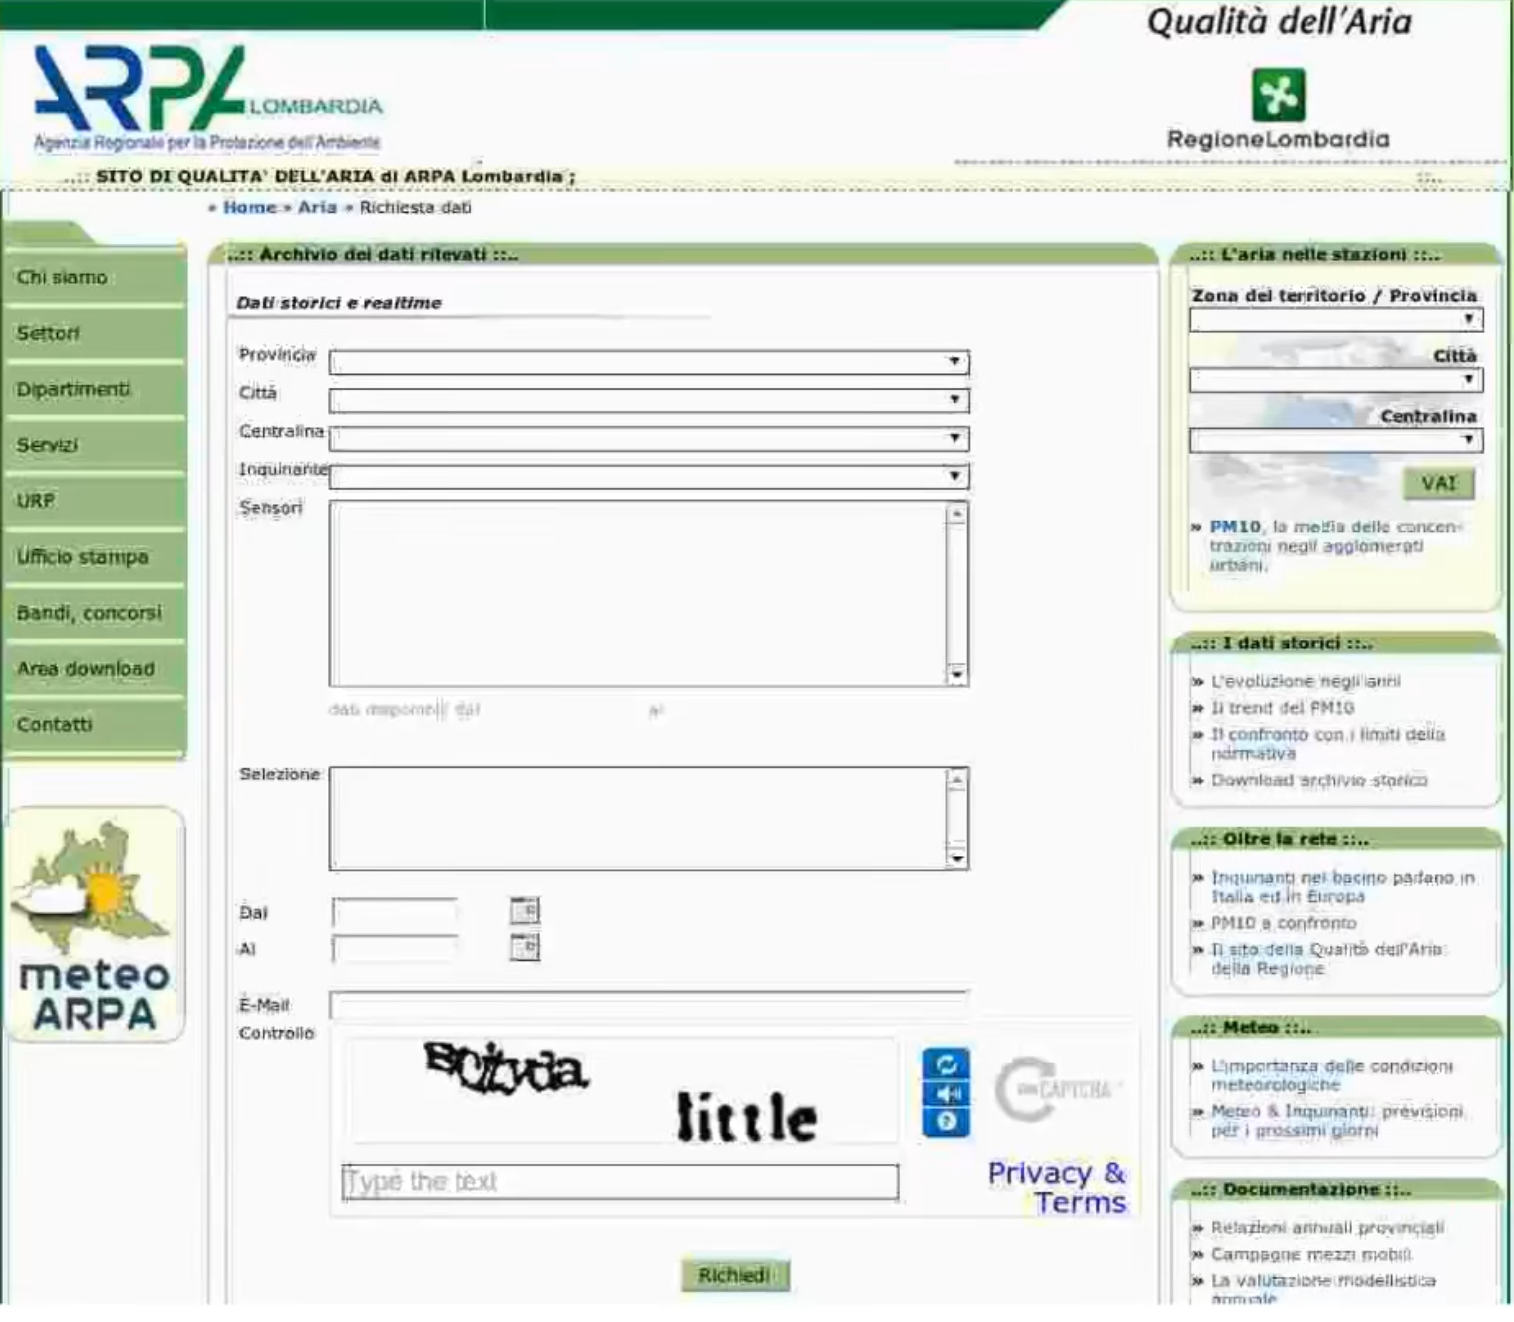
\includegraphics[width=0.7\linewidth]{img/arpa.png}\hspace*{\fill}
    \caption{Form per la richiesta di dati sul sito Arpa}
\end{figure}
\footnote{fonte: Trentini}

La garanzia di \quotestyle{poter fare i conti in tasca alle istituzioni}, è un 
valore che molto spesso è contrapposto al diritto alla privacy, anche in 
modo completamente ingiustificato, e esisterebbero numerosi vantaggi nell'obbligare 
il rilascio di più informazioni da parte di aziende e enti. 

A questo scopo sono state favorite varie iniziative per aumentare la quantità di 
dati liberi disponibile. 
Tra queste va ricordata nel 2009, negli Stati Uniti, la creazione del sito 
Data.gov\footnote{\url{https://www.data.gov/}}, 
con lo scopo di raccogliere in un'unico portale la maggior parte dei dataset 
aperti di enti americani. 
Non passerà molto tempo prima che altri paesi si uniscano al movimento. 
L'Italia in particolare creerà nel 2011 il proprio portale 
dati.gov.it\footnote{\url{https://www.dati.gov.it/}}, mentre l'Unione Europea nel 
2012\footnote{\url{https://data.europa.eu/euodp/it/home}}.

\skipline
Questo lavoro è da intendere come una dimostrazione delle analisi realizzabili 
tramite dati pubblici, e di quanti altri studi sarebbe possibile eseguire se fossero 
disponibili le informazioni mancanti.

Tra le domande che ci si porrà, ci si chiederà se il pavè, a Milano, 
influisca sull'incidentalità, o se gli autovelox rendano più attenta 
la guida dei conducenti in loro prossimità, o ancora se le linee dei trasporti pubblici 
influiscano in maniera positiva o negativa sui sinistri.

Altre questioni interessanti potrebbero essere:\\
Quali sono le strade più pericolose in Italia?\\
Si ha più probabilità di essere coinvolti in un sinistro in città o 
su una strada extraurbana?\\
Le linee di trasporto pubblico influenzano il traffico positivamente o negativamente?\\
Il numero di passeggeri influisce sulla probabilità di essere coinvolti in un 
incidente?\\
Esistono fattori di distrazione per il conducente di un'automobile? 

%%%%%%%%%%%%%%%%%%%%%%%%%%%%%%%%%%%%%%%%%%%%%%%%%%%%%%
\chapter{Origine dei dati}

\section{Dati riguardanti incidenti}

La maggior parte dei dataset utilizzati in questo lavoro 
provengono dall'Istituto nazionale di statistica, in particolare 
dall'archivio\footnote{\url{https://www.istat.it/it/archivio/87539}}
di dati non geolocalizzati su incidenti stradali in Italia.
Questo dataset contiene un'ampia gamma di campi, tra cui ora, 
mese, giorno della settimana in cui è avvenuto l'incidente, 
ma anche informazioni sui passeggeri, la natura del sinistro e il tipo di strada. 
Particolarmente interessanti sono anche i campi riguardanti la categoria di incrocio 
a cui è avvenuto il sinistro, come rettilineo, rotonda o semaforo.

\lighttext{(\\
    \indent anno, provincia, comune, giorno,\\
    \indent localizzazione\_incidente: zona incidente come urbana, extraurbana o autostrada\\
    \indent tipo\_di\_strada: numero di carreggiate della strada,\\
    \indent pavimentazione: tipo di pavimentazione,\\
    \indent intersezione\_o\_non\_interse3: tipo di intersezione,\\
    \indent segnaletica : tipo di segnaletica presente,\\
    \indent condizioni\_meteorologiche, natura\_incidente,\\
    \indent tipo\_veicolo\_a : questo campo è ripetuto per altri due veicoli,\\
    \indent veicolo\_\_a\_\_\_et\_\_conducente: questo e i due campi successivi sono ripetuti anche per i passeggeri,\\
    \indent veicolo\_\_a\_\_\_sesso\_conducente,\\veicolo\_\_a\_\_\_esito\_conducente, \\
    \indent morti\_entro\_24\_ore,\\
    \indent morti\_entro\_30\_giorni : questo insieme non contiene la categoria precedente,\\
    \indent feriti, Ora,\\
    \indent trimestre : prima del 2014 questo campo è sostituito da 'anno'\\
)}

Per quanto riguarda i dati geolocalizzati, 
la fonte è invece il giornale online TheSubmarine \cite{SUBMARINE:1}
che, in un articolo riguardante l'incidentalità a Milano, 
ha ottenuto dall'ente Istat la pubblicazione di una parte degli 
incidenti avvenuti nella città nel 2016, con la relativa posizione.
Il dataset in questione è abbastanza scarno, contiene solamente 
l'incidente con la relativa posizione, indicata tramite coordinate geografiche.

Infine l'ultimo dataset è stato trovato sul sito di 
ACI\footnote{Automobile Club Italia} \cite{ACI:1}.
Questi dati, specifici a autostrade e strade provinciali, indicano anche il 
nome della via in cui è avvenuto l'incidente, oltre a informazioni come 
l'orario, il mese o il giorno della settimana.

\lighttext{(\\
    \indent COD REG,REGIONE,\\
    \indent COD PROV,PROVINCIA,\\
    \indent NOME STRADA : codice e nome della strada,\\
    \indent INC: numero di incidenti (ce ne sono più per riga),\\
    \indent MOR,FER,\\
    \indent NVEI: numero di veicoli coinvolti\\
)}

\section{Dati riguardanti autovelox}

Una delle prime domande che ci si è posti, è stata se gli autovelox, installati 
nel tentativo di ridurre la velocità delle vetture, avessero influenza sul numero 
degli incidenti del luogo.

Un primo dataset individuato, che riguardasse delle posizioni 
degli autovelox fissi, è stata una mappa 
GoogleMyMaps\footnote{\url{https://www.google.com/maps/d/viewer?mid=1CBgMTvIDnbGo22-Y1f3rVcbeX4C0v_w1&ll=45.365557951599605\%2C10.03650113755961&z=8}} 
creata da un utente anonimo, dunque senza un modo di provare l'autenticità dei dati. 
Per evitare di fare uso di informazioni non corrette, si è preferito scartare 
questa fonte.

Il dataset utilizzato, invece, è stato ottenuto tramite OpenStreetMaps, 
realizzando una query per selezionare solo gli autovelox presenti a Milano. 
Per restringere il campo di ricerca a solo la città, si è fatto uso delle 
Overpass API\footnote{\url{https://overpass-turbo.eu/}}, 
specifiche per OpenStreetMaps, utilizzando il codice riportato nel riquadro seguente: 

\begin{code}
[out:json];
node({{bbox}})["highway"="speed_camera"];
out meta;
\end{code}

Il dataset ricavato, purtroppo, non contiene informazioni riguardanti quando gli 
autovelox siano stati installati, fattore importante per capirne l'effetto 
sul traffico e sugli incidenti.
Tuttavia il sito web ztlmilano \cite{ZTLMILANO:1}
contiene un articolo nel quale specifica una lista di 
autovelox installati nel 2014. 
Sapendo che il dataset di OpenStreetMaps è stato aggiornato fino ad oggi, 
è possibile ricavare la posizione precisa di questi ultimi.

La lista di Ztlmilano contiene i seguenti autovelox: 

\begin{center}
    \def\arraystretch{1.5}%  
    \begin{tabular}{ |c|c| } 
    \hline
    Numero & Localizzazione dell'autovelox \\ 
    \hline
    \rowcolor{TableGray}
    1   &   Viale Monteceneri  dir. Lugano\\
    2   &   Viale Monteceneri dir. Serra\\
    \rowcolor{TableGray}
    3   &   Cavalcavia del Ghisallo\\
    4   &   Viale Serra \\
    \rowcolor{TableGray}
    5   &   Viale Serra\\
    6   &   Via Fermi\\
    \rowcolor{TableGray}
    7   &   Viale Fulvio Testi direz. perif.\\
    8   &   Viale Fulvio Testi direz. centro\\
    \rowcolor{TableGray}
    9   &   Viale Palmanova  direz. centro\\
    10  &   Viale Palmanova\\
    \rowcolor{TableGray}
    11  &   Via Ferrari direz. Ripamonti\\
    12  &   Via Ferrari\\
    \rowcolor{TableGray}
    13  &   Via Chiesa Rossa\\
    14  &   Via dei Missaglia direz. centro\\
    \rowcolor{TableGray}
    15  &   Via dei Missaglia direz. periferia\\
    16  &   Viale Famagosta\\
    \rowcolor{TableGray}
    17  &   Via Parri\\
    18  &   Via Parri\\
    \hline
    \end{tabular}
    \label{ztl-milano}
\end{center}

Il campi della tabella ripetuti sono dovuti al fatto che alcuni autovelox sono stati 
installati in entrambe le direzioni.

\section{Dati riguardanti patentati}

Un'importante necessità in un indagine di questo tipo, è avere un contesto con cui 
interpretare i risultati ottenuti. 
Non è possibile, per esempio, dire se su una certa strada si ha un numero alto di 
incidenti, senza sapere quante automobili passano in una giornata.

Si è dunque tentata una ricerca, infruttuosa, di dataset sul traffico stradale nel periodo 
dal 2010 al 2018.
Queste informazioni si sono cercate, principalmente per la zona di Milano, nei principali 
siti di open data, con parole chiave come \quotestyle{traffico milano} e 
\quotestyle{flussi autostrade}. 
Si è inoltre controllato sul sito di Autostrade per 
l'Italia\footnote{\url{http://www.autostrade.it/it/home}}, 
ma le uniche informazioni trovate sono in tempo reale.

Non avendo trovato alcuna informazione sull'argomento, si è tentato di realizzare 
alcune stime del numero di automobili per regione, e a Milano.

I dati sui patentati per regione, che è stato utilizzato per stimare il traffico 
regionale, proviene dal sito del Ministero delle Infrastrutture e 
Trasporti\footnote{\url{http://dati.mit.gov.it/catalog/dataset/patenti}}.
Questo dataset è diviso in vari file seconda della regione e, vista la quantità 
non necessaria di informazioni, si è preferito usare una sintesi di questi provienienti da 
un'infografica che sintetizza i dati in questione \cite{INFOGRAFICA_MIT:1}.
In particolare, da questo file pdf si è mantenuto solamente il numero di patenti per regione.

\'E anche necessario chiedersi quanto il numero dei patentati per regione sia un 
fattore valido con cui stimare il traffico, tenendo conto del fatto che molte 
persone non vivono nella regione 
in cui hanno ottenuto la patente, e altre potrebbero spostarsi ogni giorno in altri 
luoghi per questioni di lavoro. 
Va dunque tenuto conto che questa stima non sarà probabilmente tra le più accurate, 
e in caso di grandi disparità tra regioni, si potrebbe dover invalidare i calcoli eseguiti.

\section{Dati riguardanti l'area C}

Per lo stesso motivo del capitolo precedente, si sono cercate informazioni sugli 
accessi all'area C di Milano per realizzare una stima approssimativa del traffico, in 
città, in base all'orario.

Il dataset riguardante gli accessi è stato trovato sul sito di open data del comune di 
Milano\footnote{\url{https://dati.comune.milano.it/organization/comunedimilano?q=area+c&sort=score+desc\%2C+metadata_modified+desc}}, 
dove sono disponibili varie tipologie di file distinti, per esempio, per orario, 
mese o località. 
Tra questi si è utilizzata la tipologia contenente orari e data dell'accesso.

\lighttext{(\\
    \indent year : anno dell'accesso in area C,\\
    \indent month: mese dell'accesso in area C,\\
    \indent day: giorno dell'accesso in area C,\\
    \indent hour: ora dell'accesso in area C,\\
    \indent totale: numero di accessi nella riga,\\
    \indent areac: booleano che indica se l'area C sia attiva o meno\\
)}

Oltre ai dati riguardo agli accessi all'area C, si è fatto uso anche di una mappa 
raffigurante i varchi di entrata e i limiti del centro storico, 
proveniente dal sito del comune di 
Milano\footnote{\url{https://www.comune.milano.it/aree-tematiche/mobilita/area-c}}. 

Per quanto anche questa stima non sia tra le più accurate, ci si può aspettare che 
il numero di accessi corrisponda, almeno in piccola parte, al traffico di Milano.

\section{Dati riguardanti le zone di Milano}

I dataset delle zone geolocalizzate di Milano provengono dal geoportale del comune di 
Milano\footnote{\url{https://geoportale.comune.milano.it/}}, e contengono i poligoni che 
costituiscono i municipi della città, 
oltre a informazioni sulla superficie e il perimetro delle zone.

\lighttext{(\\
    \indent MUNICIPIO: id della zona,\\
    \indent AREA : della zona,\\
    \indent PERIMETRO: della zona,\\
    \indent geometry: insieme di punti che formano il poligono\\
)}

Questi dati sono utili a determinare, a grandi linee, quali sono le zone con più incidenti 
a Milano, nonostante il risultato ottenuto non sarà mai troppo preciso, soprattutto 
per l'ampiezza delle sezioni rispetto al numero di strade di ogni sezione.

Un altro problema, è che le zone non contengono solamente la superficie stradale, ma anche 
abitazioni e terreni, in cui non avverranno mai incidenti.
Sarà necessario tenere a mente, che il numero di incidenti per zona che verrà ricavato, 
è da considerarsi come una stima \quotestyle{dal basso}, se contrapposto all'area del municipio, 
e stime che utilizzano solamente la superficie stradale avranno inevitabilmente volume 
di incidenti per chilometro maggiore.

\section{Dati riguardanti il meteo}

Per quanto riguarda i dati su meteo, si è tentato di utilizzare le informazioni 
provenienti dalle centraline Arpa. 
Dopo una veloce analisi, la cui mappa è visibile in figura \ref{fig:centraline-arpa}, 
si è notato il dataset non contiene tutte le stazioni di Milano.

\begin{figure}
    \hfill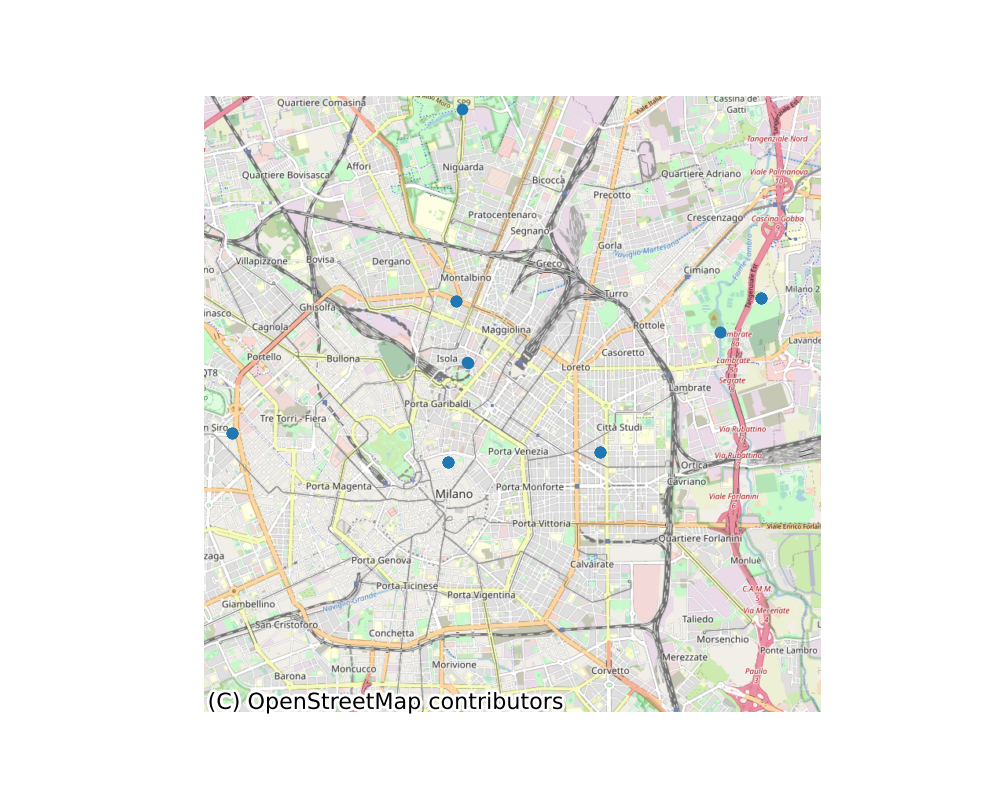
\includegraphics[width=0.7\linewidth]{../src/meteo/centraline_arpa.png}\hspace*{\fill}
    \caption{Centraline Arpa a Milano}
    \label{fig:centraline-arpa}
\end{figure}

Per esempio, utilizzando una lista di centraline meteo completa, come quella su 
Centrometeolombardo\footnote{\url{http://www.centrometeolombardo.com/content.asp?CatId=272&ContentType=Stazioni}}, 
si nota che mancano quelle di Abbiategrasso Sud e Cardorna.

Inoltre, per mancanza di dati precisi sul giorno degli incidenti, è superfluo avere 
informazioni con posizione così precisa.
Si è dunque optato per un dataset contenente temperature, umidità, e velocità del vento, 
trovato sul sito Zenodo\footnote{\url{https://zenodo.org/record/3992354}}.

Il dataset contiene i campi di cui si è parlato, misurati ogni 
ora a Milano, a partire dal 2008, fino al 2018.

\lighttext{(\\
    \indent Date\_Time: campo che contiene giorno, mese e anno,\\
    \indent Temperature: in gradi Celsius,\\
    \indent Dew\_Point: temperatura di condensazione,\\
    \indent Humidity : umidità,\\
    \indent Wind\_Speed : velocità del vento\\
)}

\section{Dati riguardanti trasporti pubblici}

Un altro fattore su cui ci si è chiesti l'influenza sull'incidentalità, è la 
presenza, nella via o viale, di trasporti pubblici in una città come, 
per esempio, Milano.

I dati riguardanti questi ultimi, hanno due provenienze, i primi sono 
dati riferiti alle linee ATM, scaricati sul sito del comune di 
Milano\footnote{\url{https://dati.comune.milano.it/dataset/ds532-atm-composizione-percorsi-linee-di-superficie-urbane}}.

\lighttext{(\\
    \indent linea: numero della linea,\\
    \indent mezzo: bus, filobus o tram,\\
    \indent percorso: identificatore del percorso,\\
    \indent verso, nome,\\
    \indent tipo\_perc: Canonico o Barrato,\\
    \indent lung\_km, num\_ferm,\\
    \indent geometry: insieme di linee che formano i percorsi\\
)}

Dallo stesso sito proviene anche il dataset riguardante gli autobus turistici, che 
contiene, in particolare, le aree di 
sosta\footnote{\url{https://dati.comune.milano.it/dataset/ds740_sosta_bus_gt_turistici}}.
Si è anche fatto uso di un dataset contenente 
solamente le linee tranviarie, trovato sul geoportale del comune di 
Milano\footnote{\url{https://geoportale.comune.milano.it/ATOM/SIT/DBT2012/DBT2012_STRATO_01_Dataset_1.xml}}.
Questo dataset è molto ampio e contiene altri livelli di informazioni, tra cui per esempio, 
le strade, le ferrovie o le piste ciclabili passanti per Milano. 

La principale funzione di questi dataset è l'ottenere i percorsi delle linee di trasporto pubblico, 
per confrontare il numero di incidenti, nelle vie in cui viaggiano autobus, rispetto a 
quelle in cui sono presenti solo autovetture private.

\section{Dati riguardanti autostrade e manto stradale}

Per la realizzazione di alcune mappe, nelle quali sono necessari i tracciati delle principali 
autostrade, si è tentata la ricerca di dati geolocalizzati sulle strade Italiane.

Il primo dataset individuato, riguardante il manto  stradale, è stato trovato sul sito 
internet dell'ente  
ANAS\footnote{\url{http://dati.mit.gov.it/catalog/dataset/grafo-stradale-anas}}. 
Tuttavia, consisteva in un file molto grande, contenente tutte le principali 
strade in Italia, e dalla precisione superflua per le mappe che si sta tentando di ottenere.

Si è dunque tentato di utilizzare il dataset presente sul geoportale del comune di 
Milano\footnote{\url{https://geoportale.comune.milano.it/}}, 
contenente anch'esso troppe strade in quanto traccia l'intero manto stradale della città.

Come ultima risorsa, si è deciso di tracciare alcune mappe in 
\textbf{geojson}\footnote{Formato di file, derivato da \textbf{Json}, cioè 
JavaScript Object Notation, utilizzato spesso per il salvataggio di informazioni, ma 
in aggiunta permette di memorizzare insiemi di punti, sotto forma di linee o poligoni, 
tramite l'apposito campo \columnstyle{geometry}.} utilizzando 
Geojson.io\footnote{\url{https://geojson.io/}}, in particolare nella zona di Milano, 
per le principali autostrade, tangenziali e strade statali. 
Allo stesso modo, Geojson.io è stato utile a tracciare alcune aree in centro a Milano, 
per confrontare gli incidenti su pavè agli incidenti su asfalto.

\section{Dati riguardanti il turismo}

Le informazioni riguardanti il turismo, sono state utili a capire se nelle annate più 
recenti, fosse presente un incremento di persone in ferie in località di montagna.

I dati sul turismo in Italia, sono stati trovati nell'archivio Istat sul 
tema\footnote{\url{https://www.istat.it/it/archivio/16777}}.
Il dataset originale era in formato xls, contenente informazioni a partire dal 1995 
fino al 2019, sia regione per regione, sia divise per nord, centro e sud.
A loro volta, i file sono divisi in più tabelle, ognuna rafficurante un particolare 
indicatore, come produttività del lavoro, turismo nei mesi non estivi, 
tasso di turisticità\footnote{Il tasso di turisticità misura il livello di "affollamento" 
turistico in un determinato periodo (anno o mese) indicando il numero di turisti presenti 
ogni 100.000 abitanti. \cite{ONTIT:1}} 
e valore aggiunto del turismo.

Per controllare la tendenza, sono stati necessari i dati regione per regione, 
a partire dal 2010 fino al 2018, convertiti in formato csv, e sono stati scelti gli 
indicatori di turismo nei mesi non estivi, e tasso di turisticità. 

\section{Immagini del traffico}

Le immagini raffiguranti il traffico in tempo reale sono prese da Google 
Maps\footnote{\url{https://www.google.com/maps/}}. 
In primo luogo, si è tentato di realizzare degli screenshot direttamente dal sito, 
tuttavia immagini prese in questo modo, contengono molti punti di interesse e altri simboli, 
che coprono informazioni importanti, come i nomi delle strade.

Per rimuovere le informazioni superflue, si è fatto uso delle API di Google Maps, 
tramite il sito Jsfiddle\footnote{\url{https://jsfiddle.net/} Un sito web che permette di 
scrivere e eseguire codice JavaScript.}.

Gli screenshot realizzati rappresentano le zone dei Navigli e dell'incrocio tra viale 
Bianca Maria e viale Ventidue Marzo.

%%%%%%%%%%%%%%%%%%%%%%%%%%%%%%%%%%%%%%%%%%%%%%%%%%%%%%
\section{Dati mancanti}

\subsection{Dati riguardanti pavè}

Nonostante le ricerche nei principali siti di opendata
\footnote{
    \url{https://dati.comune.milano.it/dataset}, 
    \url{https://www.dati.lombardia.it/},
    \url{https://www.dati.gov.it/}
    }
non sembra che esista un dataset contenente informazioni sulla composizione del 
manto stradale di Milano. 
In particolare, si sono cercate le informazioni tramite parole chiave come 
\quotestyle{strada}, \quotestyle{manto stradale}, \quotestyle{pave}, 
\quotestyle{composizione strada}.

Una risorsa trovata durante le ricerche, è una mappa utilizzata in un articolo del blog online 
Urbanfile \cite{URBANFILE:1}. 
Dopo una rapida consultazione con l'autore tuttavia, non risulta esserci alcun 
dataset contenente informazioni riguardanti il pavè a Milano, infatti la cartina è 
stata realizzata per conoscenza personale.

Il dataset che potrebbe avvicinarsi di più alle informazioni ricercate, 
potrebbe essere quello riguardante i percorsi dei trasporti tranviari. 
Basandosi su queste informazioni, e assumendo che la maggior parte delle linee dei 
tram a Milano siano in pavè, è possibile ottenere un dataset con taglia discreta.

Tuttavia, confrontando il dataset delle linee tranviarie ottenuto, 
con la mappa di Urbanfile, per quanto alcune linee coincidano, non si è trovata 
somiglianza sufficiente per giustificare l'utilizzo.

Come ultima spiaggia, si è deciso di tracciare una mappa utilizzando 
Geojson.io\footnote{\url{https://geojson.io/}}, come già fatto per le autostrade a Milano, 
basandosi sulla cartina trovata su Urbanfile. 

\subsection{Dati riguardanti traffico stradale}

Per quanto riguarda i dati sul traffico stradale, anche in questo caso non è stato trovato un 
dataset, sia nei siti di cui si è parlato in precedenza, sia su quello di 
autostrade\footnote{\url{http://www.autostrade.it/it/home}}.

Il primo tentativo, per avere una stima del traffico è stato la realizzazione di uno 
script per fare scraping da Google Maps. 
Quest'ultimo infatti mostra sia il traffico in tempo reale, sia 
il traffico stimato a una determinata ora. 
Tuttavia, leggendo nella documentazione, si è scoperto che non è possibile ottenere 
dati sul traffico abituale, per la mancanza delle API corrispondenti. 
Invece, per quanto riguarda il traffico in tempo 
reale, questo è disponibile, ma non è particolarmente utile per la quarantena dovuta al 
Covid-19, che riduce notevolmente il volume di automobili. 
Per quanto fosse stato possibile realizzare comunque uno script per effettuare scraping della 
quantità di traffico nelle strade, registrando il colore delle direttrici per ogni orario della 
giornata nei periodi interessati, si è optato per la ricerca di un altro dataset.

Si è deciso, dunque, di utilizzare i dati riguardanti gli ingressi in area C, 
trovati sul sito del comune di Milano\footnote{\url{https://dati.comune.milano.it/dataset}}, 
nonostante questi non permettano una stima perfetta.

Un'altro dataset utilizzato per stimare il numero di automobili, è quello contenente 
il numero di patentati per regione, trovato nel sito del Ministero dei 
Trasporti\footnote{\url{dati.mit.gov.it/catalog/dataset/patenti}}.
I dati, riguardanti i patentati fino al 2019, sono divisi in file per regione e 
contengono anche informazioni riguardanti la provincia e data di conseguimento della 
patente, oltre al tipo di ceritificato ottenuto.

\subsection{Dati su strade, incroci, semafori}

In alcuni capitoli, in particolare quelli riguardanti le tipologie di incidente e 
di incrocio, i dati non disponibili, sono soprattutto quelli sul 
numero di strade per le diverse categorie.

Per la trovare questi ultimi si è cercato, innanzi tutto, articoli o dataset online, con 
parole chiave come \quotestyle{numero semafori Milano} o \quotestyle{strade incroci semafori}.
Non trovando alcun riscontro, si è ricercato l'argomento nei principali siti contenenti 
dataset, di cui si è parlato in precedenza. 

Le informazioni più vicine a ciò che si stava cercando, sono state trovate sul geoportale 
del comune di Milano, nei dati sul manto stradale.
Questo dataset contiene vari layer di informazioni, tra cui 
\columnstyle{Area di circolazione veicolare}, 
\columnstyle{Area di circolazione pedonale} e \columnstyle{Area di circolazione ciclabile}, 
tuttavia, in nessuno di questi livelli, si sono trovate informazioni utili a dividere, 
per esempio, intersezioni segnalate da incroci con semaforo. 

Inoltre, per la maggior parte dei livelli, non si sono trovate informazioni sul significato 
delle colonne presenti nei dataset come, per esempio, \columnstyle{GZ\_STR\_TY} o 
\columnstyle{GZ\_STR\_TYF}. 

Le ricerche per un file contenente informazioni sui metadati sono state eseguite sia 
sul sito del comune di Milano sia, in generale, tramite motore di ricerca, con parole chiave 
come \quotestyle{ID\_ZRIL milano} o \quotestyle{ID\_ZRIL metadati}. 
Nel caso di quest'ultimo, si è ipotizzato, tracciando una parte dei valori della colonna, 
che fosse un identificatore univoco del territorio, ipotesi confermata da un pdf trovato sul sito 
cittametropolitana\footnote{\url{https://www.cittametropolitana.mi.it/export/sites/default/DeCiMetro/DOCUMENTI-DA-SCARICARE/Manuale-civici.pdf}}. 

%%%%%%%%%%%%%%%%%%%%%%%%%%%%%%%%%%%%%%%%%%%%%%%%%%%%%%
\chapter{Dati Geolocalizzati}

\section{Incidenti}

I dati riguardanti gli incidenti geolocalizzati, sono disponibili in un dataset contenente una 
lista di punti indicanti latitudine e longitudine dell'incidente. 
Ciò che delude, è che non è presente nessuna informazione aggiuntiva, se non la posizione 
dell'incidente.

Controllando i dati trovati, in particolare come questi siano posizionati, 
si nota, dalla mappa destra nella figura \ref{fig:heatmap-municipi} come, 
gli incidenti a Milano siano distributi con concentrazioni più alte, 
in alcuni punti di interesse della città, come Piazzale Loreto, Zona Navigli 
e Monumentale, e Corso Ventidue Marzo.

Sarebbe interessante sapere se esistano zone con maggiore concentrazione di incidenti rispetto 
alla media, e ottenere un indice numerico della pericolosità di una determinata zona.

Nella mappa sinistra della figura \ref{fig:heatmap-municipi}, si è divisa la città di Milano 
in base ai diversi municipi, ed è possibile osservare che nel centro storico si hanno la 
maggior parte degli incidenti.

\begin{figure}
    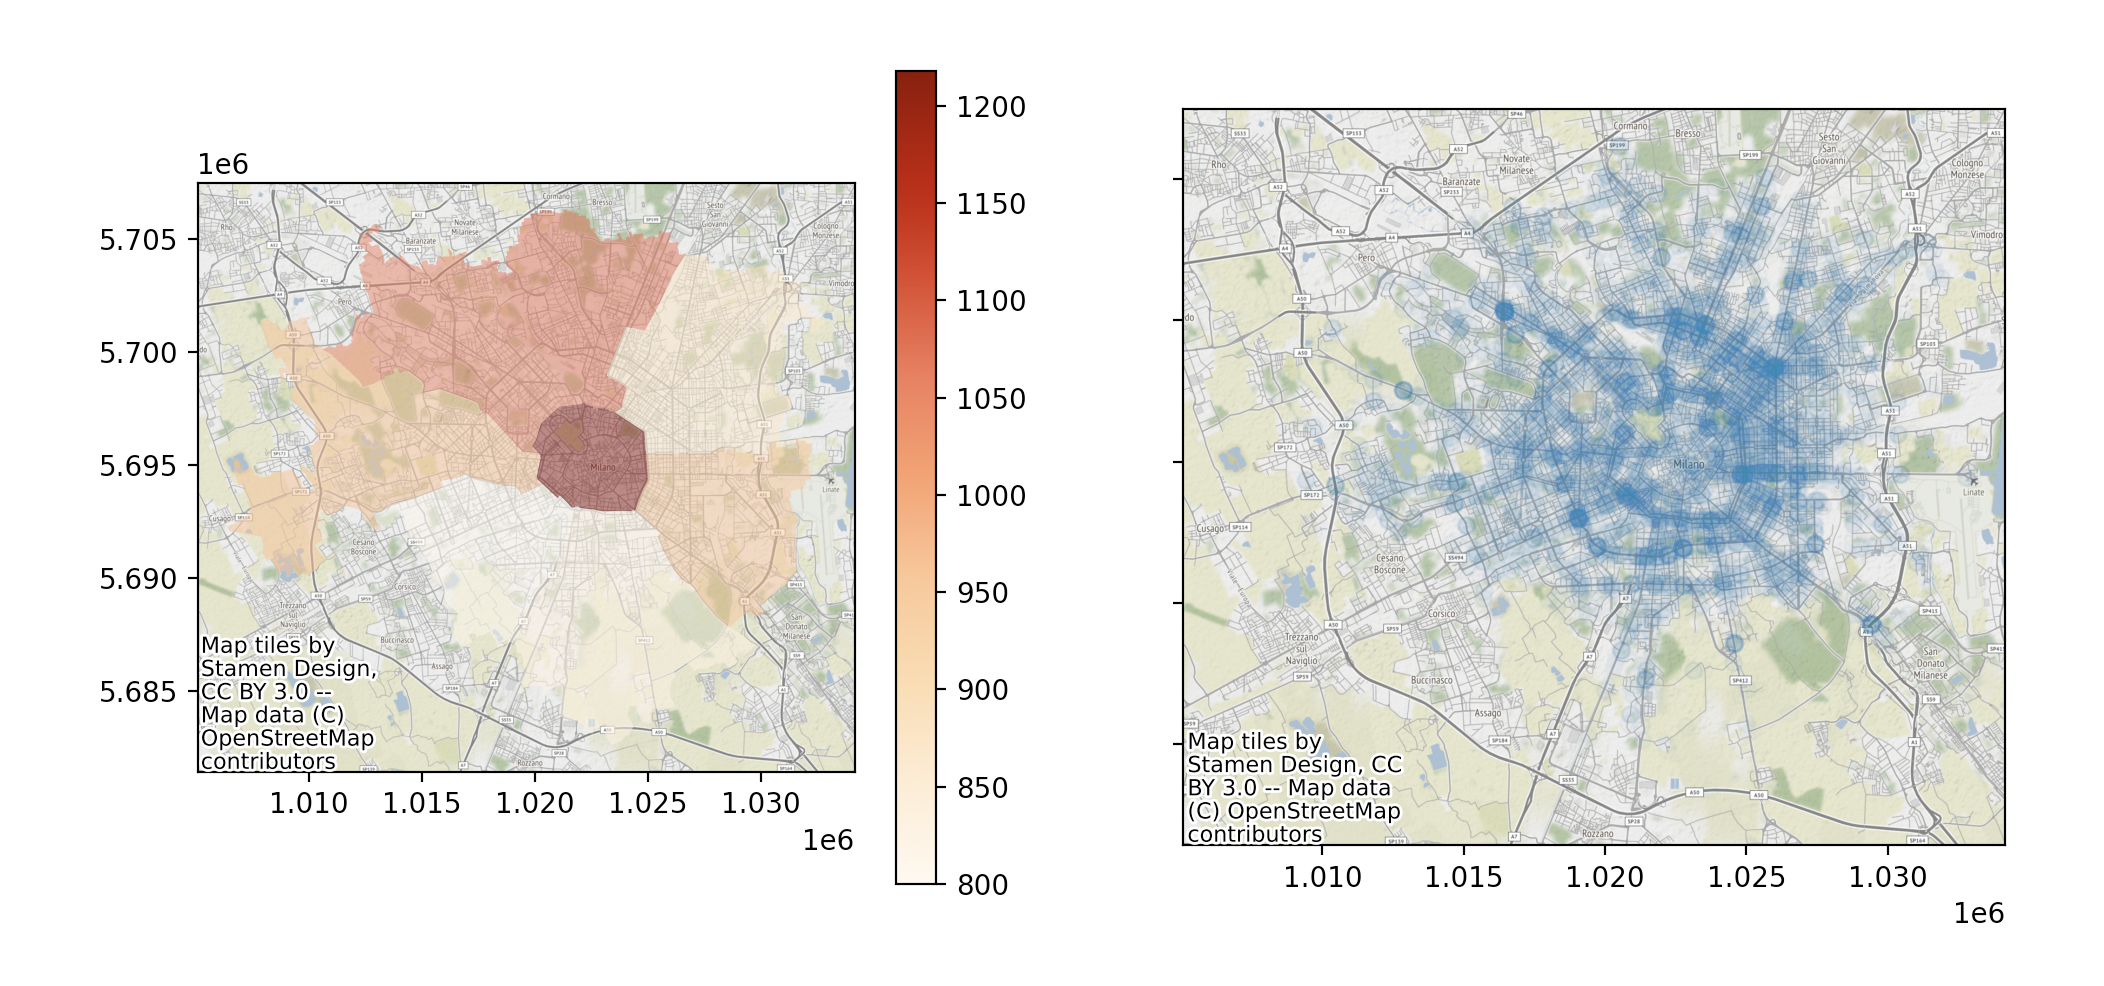
\includegraphics[width=\linewidth]{../src/municipi_milano/incidenti_municipio.png}
    \caption{Incidenti a Milano per municipio}
    \label{fig:heatmap-municipi}
\end{figure}

Non tutte le zone hanno la stessa superficie, e ovviamente sezioni più ampie hanno un maggior 
numero di strade. Avendo a disposizione l'area dei vari municipi, 
è possibile calcolare la media di incidenti al chilometro quadrato per zona.
I risultati sono riportati negli istogrammi sottostanti.

\begin{code}    
inc = gp.GeoSeries(df).sort_index()

area = pd.Series(data['AREA'], index=data['MUNICIPIO'])
incidenti = pd.Series(inc, index=inc.index)

# trasformazione in chilometri quadri
incidenti_per_zona = (incidenti / area) * 1000000 
\end{code}

\begin{figure}
    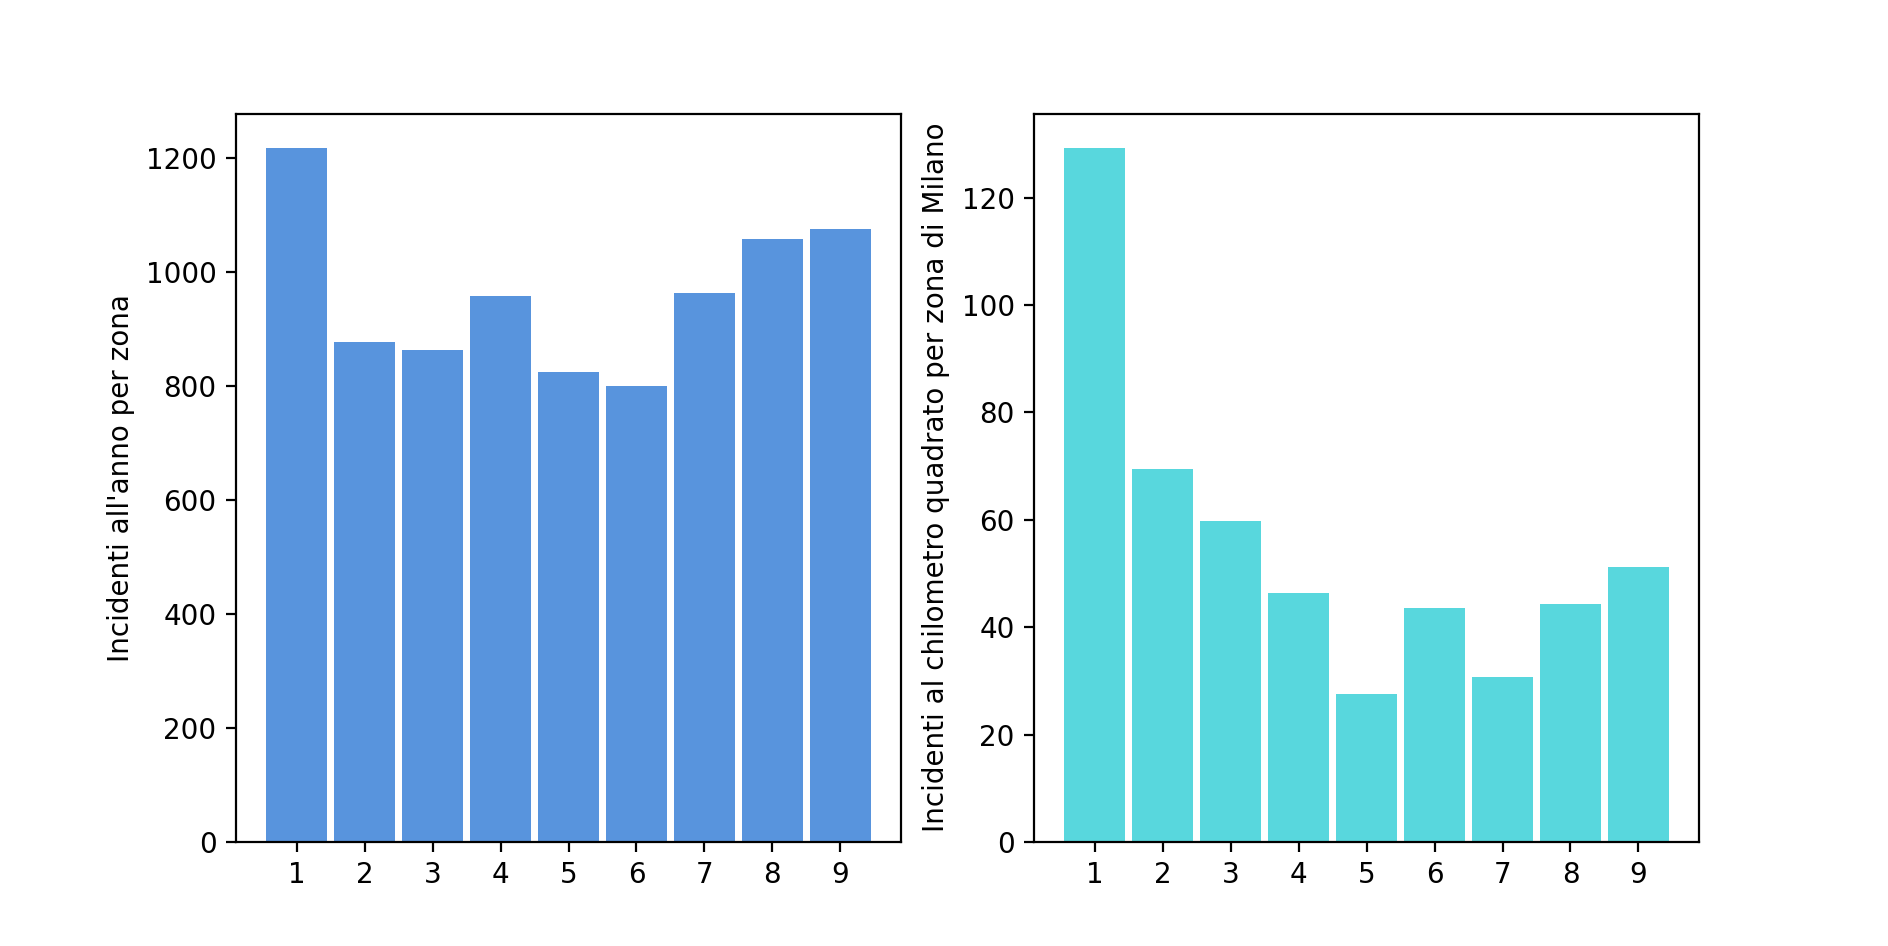
\includegraphics[width=\linewidth]{../src/municipi_milano/incidenti_superf.png}
    \caption{Incidenti a Milano per zona e in base alla superficie della zona}
    \label{fig:incidenti-chilometro}
\end{figure}

Nella figura \ref{fig:incidenti-chilometro} spicca, sia nel grafo di sinistra, rappresentante 
il numero di incidenti totali per zona, che in 
quello di destra, che contiene il numero di incienti divisi per l'area del municipio, 
la zona 1, cioè quella del centro storico, vista la superficie minore 
rispetto agli altri municipi.

Una volta creata la tendenza generale del municipio, è possibile confrontare i risultati 
ottenuti con il numero di incidenti in zone più ristrette, per esempio attorno a piazzale Loreto.

\begin{figure}
    \hfill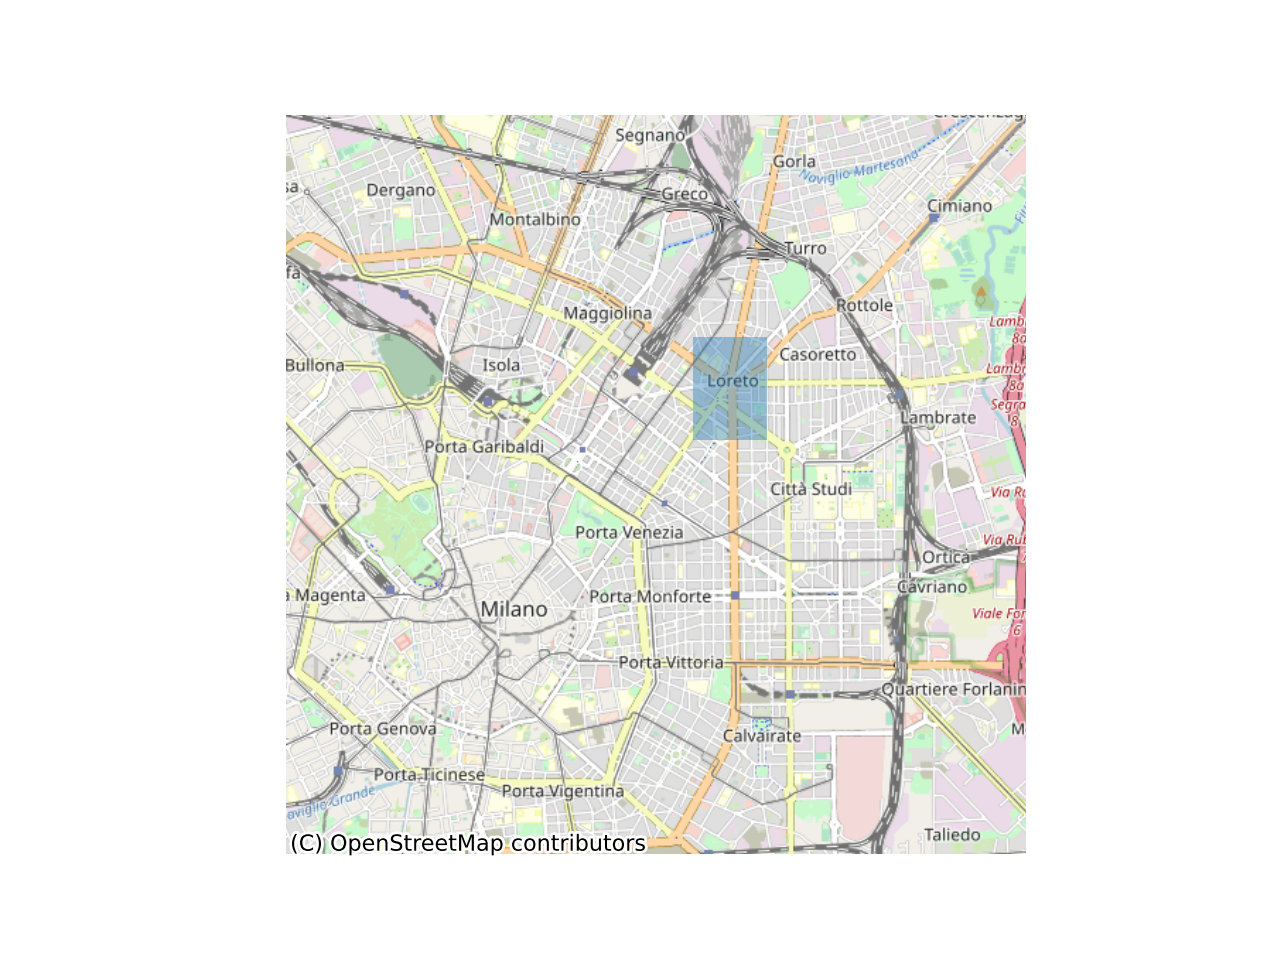
\includegraphics[width=0.7\linewidth]{../src/municipi_milano/zona_loreto.png}\hspace*{\fill}
    \caption{Zona presa in considerazione per piazzale Loreto}
    \label{fig:zona-loreto}
\end{figure}

\begin{code}
loreto = geometry.Polygon([p1, p2, p4, p3])

loreto_incidenti = 0
for point in incidenti['geometry']: 
    point = geometry.Point(point)

    if loreto.contains(point): 
        loreto_incidenti += 1

area_loreto = loreto.area * data['AREA'].iloc[0] / geometry.Polygon(data['geometry'].iloc[0]).area
area_loreto_inc = loreto_incidenti * 1000000 / area_loreto
\end{code}

Il numero di incidenti per chilometro che risultano, nell'area considerata in figura 
\ref{fig:zona-loreto}, sono $231.06$, considerando che il massimo ottenuto per zona, 
il centro storico, arriva attorno a $120$ incidenti per chilometro quadrato, è possibile affermare 
che Piazzale Loreto sia una zona ad alta incidentalità.

Va anche tenuto in considerazione che, come spiegato nel capitolo sull'origine dei dati, 
prendendo una qualsiasi area di strade, si avrà un numero di incidenti per chilometro quadrato 
molto maggiore rispetto a quello delle aree municipali, per la presenza di zone dove  
le automobili non possono viaggiare, come gli edifici.

Una domanda che sorge spontanea è, perchè nel centro storico risulta tra le aree con maggiore 
incidentalità, il volume di traffico, e quindi di incidenti, non dovrebbe essere abbassato 
della presenza dell'area C?

\begin{figure}
    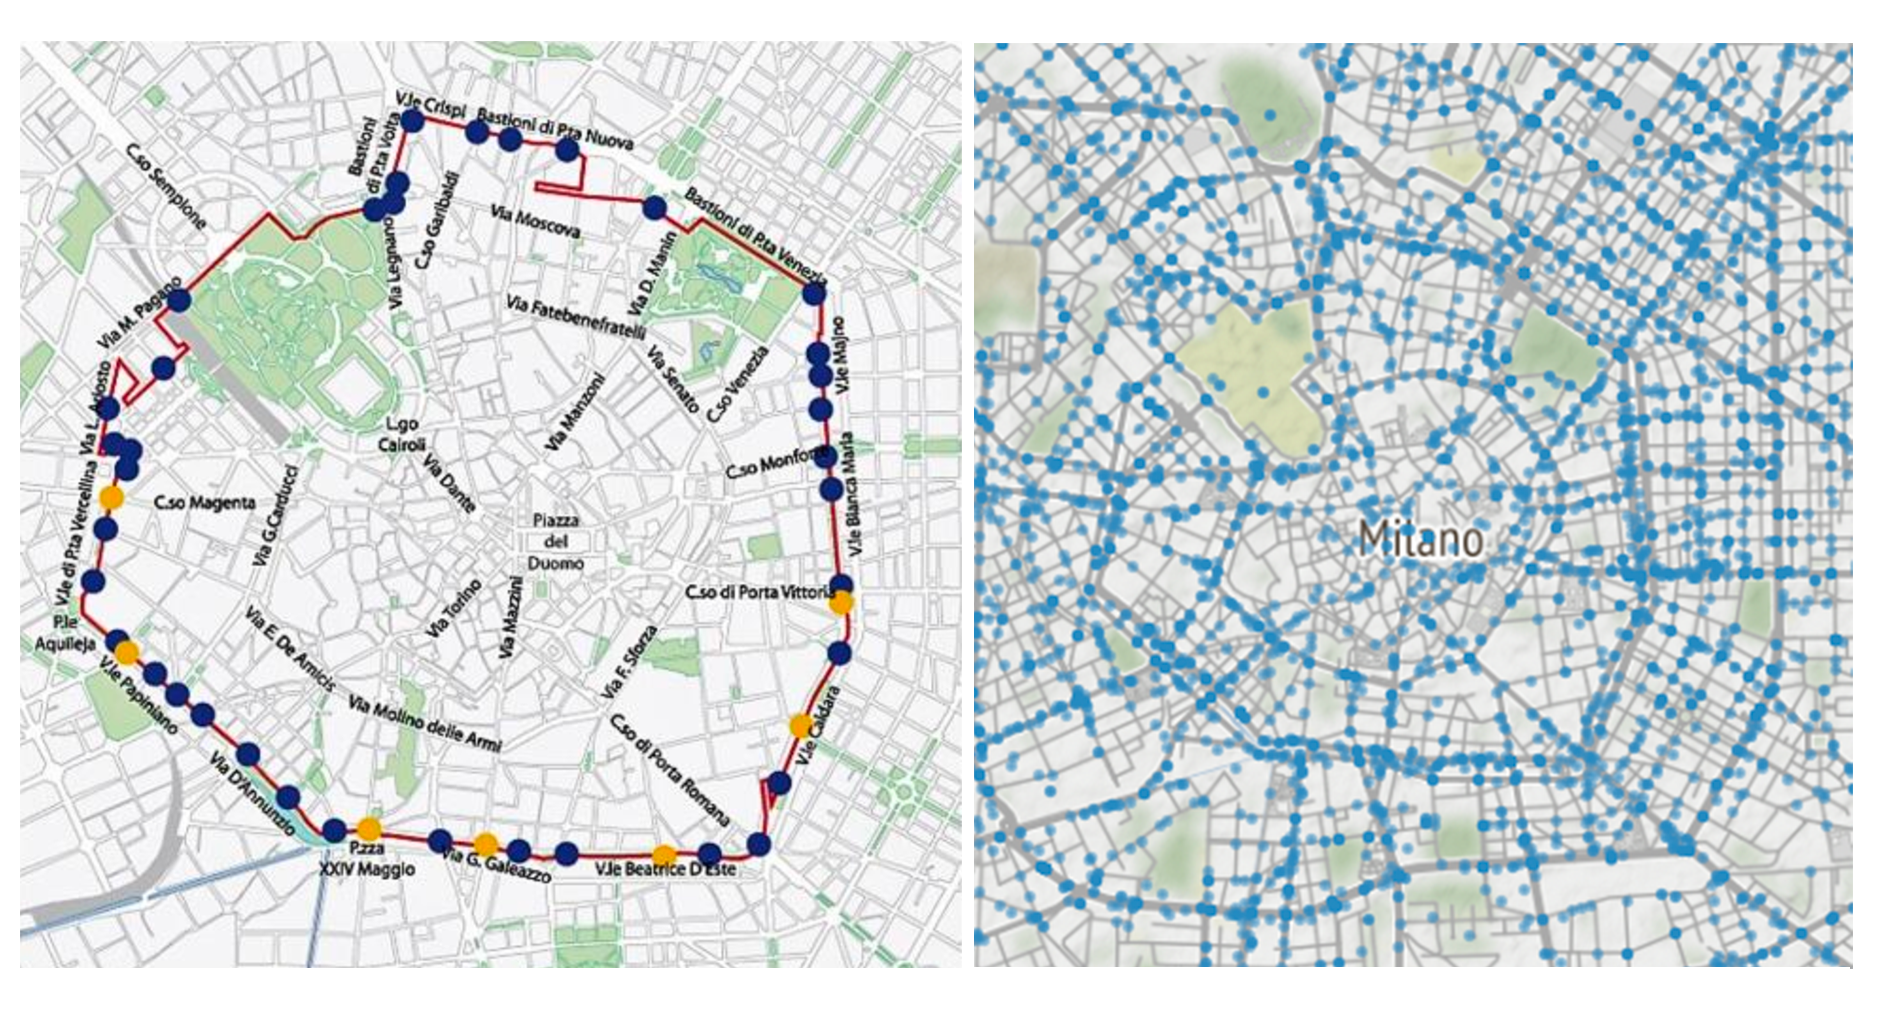
\includegraphics[width=\linewidth]{../src/area_c/area_c_incidenti.png}
    \caption{Perimetro dell'area C e incidenti nella stessa zona}
    \label{fig:perimetro-area-c}
\end{figure}

Dopo più attenta osservazione del perimetro dell'area C, visibile nell'immagine a sinistra nella 
figura \ref{fig:perimetro-area-c}, si osserva che la maggior parte degli 
incidenti avvengono sulla circonvallazione interna, 
situata fuori dall'area C, ma compresa nel centro storico di Milano.

Prendendo in considerazione solamente l'area C, il numero di incidenti scende a $46.83$ 
per chilometro quadrato, di gran lunga minore rispetto al valore del centro storico, 
dunque è possibile concludere che la riduzione del traffico nel centro di Milano ha impatto 
consistente sull'incidentalità.

%\clearpage
\section{Incidenti e Linee dei Trasporti Pubblici}

Il dataset dei tragitti dei trasporti pubblici copre molta più superficie rispetto a 
quello degli incidenti, dopo aver eliminato alcune linee di autobus che risultavano 
troppo in periferia, si ottiene la mappa sinistra nella figura \ref{fig:geo-trasporti}: 

\begin{figure}
    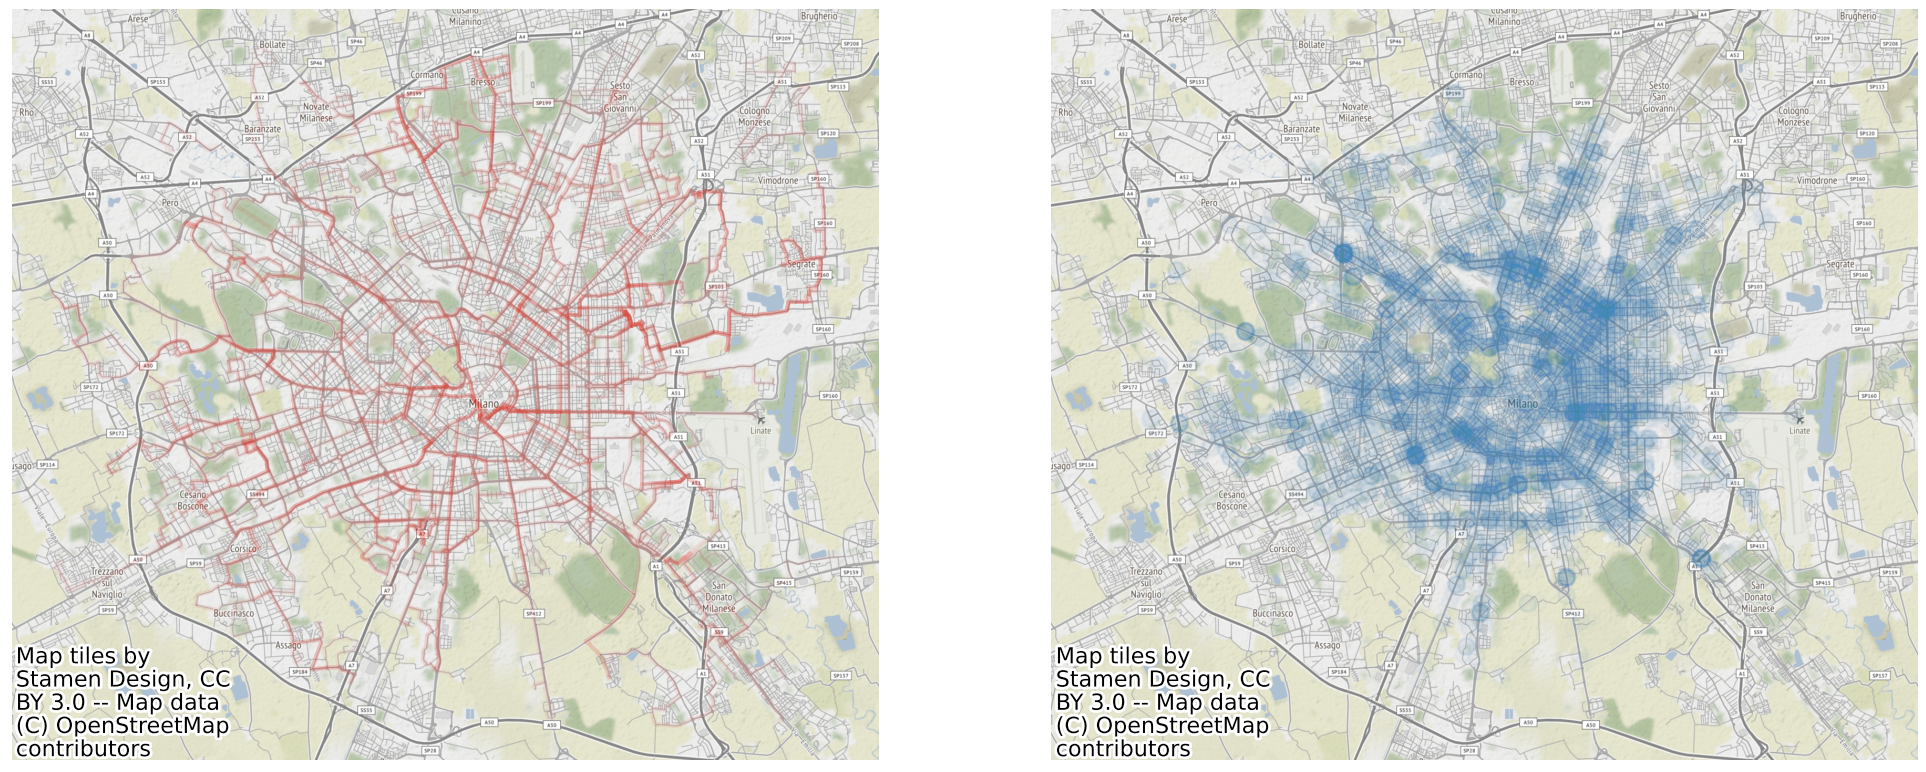
\includegraphics[width=\linewidth]{../src/atm/linee_atm.png}
    \caption{Linee Autobus e Tram a Milano}
    \label{fig:geo-trasporti}
\end{figure}

Affiancando le posizioni degli incidenti ai tragitti dei trasporti pubblici, 
non è possibile notare un collegamento preciso tra i due dataset. 
Sono presenti tuttavia alcune corrispondenze come, per esempio, la zona dei Navigli 
e quella circostante a Corso Ventidue Marzo. 

Un fenomeno interessante, è la presenza di alcune strade con alta incidentalità, 
parallele a linee di autobus. 
Un esempio è quello di zona Navigli, in figura \ref{fig:navigli}, dove le vie interessate sono:
Viale Gian Galeazzo e Viale Beatrice D'Este, parallele a Viale Col di Lana e Viale Bligny.
Lo stesso fenomeno è osservabile su Viale Gabriele D'Annunzio e Viale Gorizia e Coni Zugna, 
e nella zona vicino a corso Ventidue Marzo.

\begin{figure}
    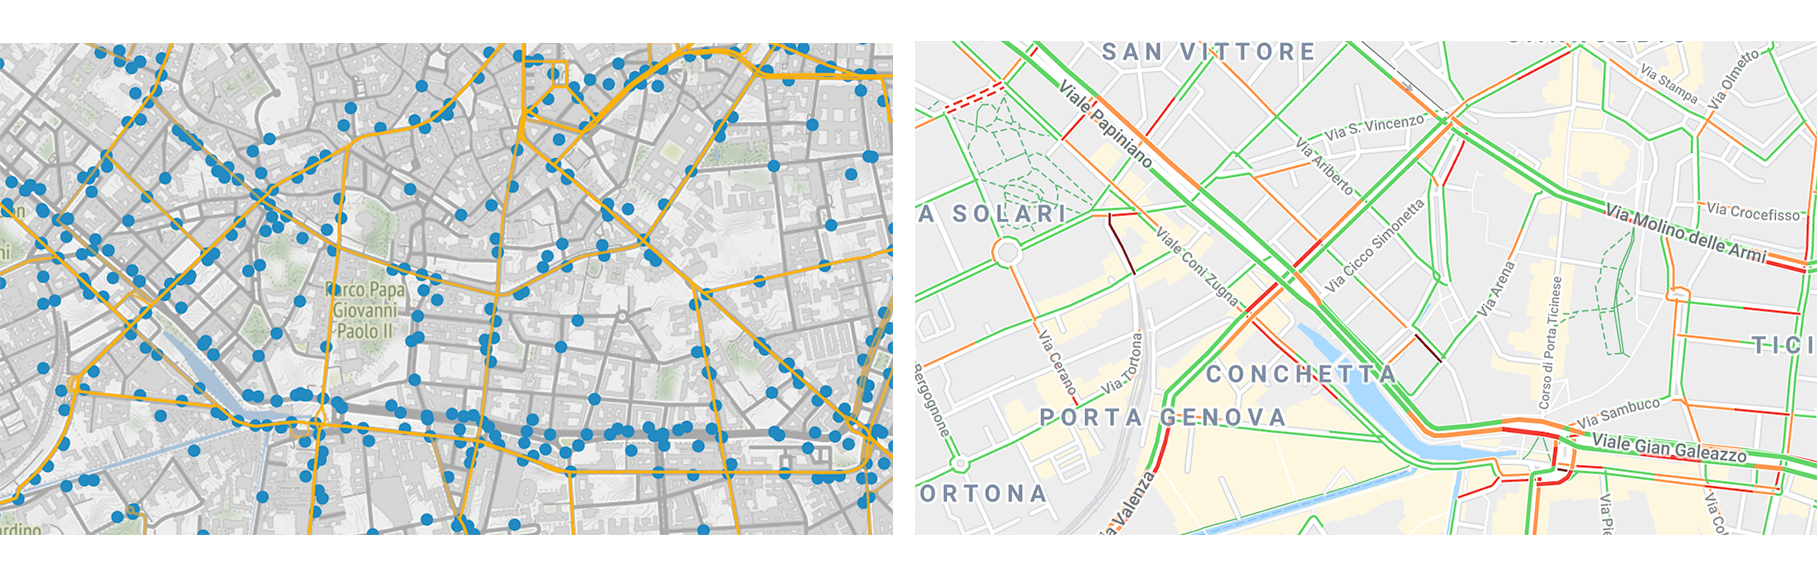
\includegraphics[width=\linewidth]{../src/atm/navigli.png}
    \caption{Linee dei trasporti pubblici e condizioni di traffico nella zona Navigli}
    \label{fig:navigli}
\end{figure}

Anche vicino a corso Ventidue Marzo, nella mappa \ref{fig:22-marzo} si può 
notare lo stesso fenomeno, tra Viale Bianca Maria e Viale Premuda.

\begin{figure}
    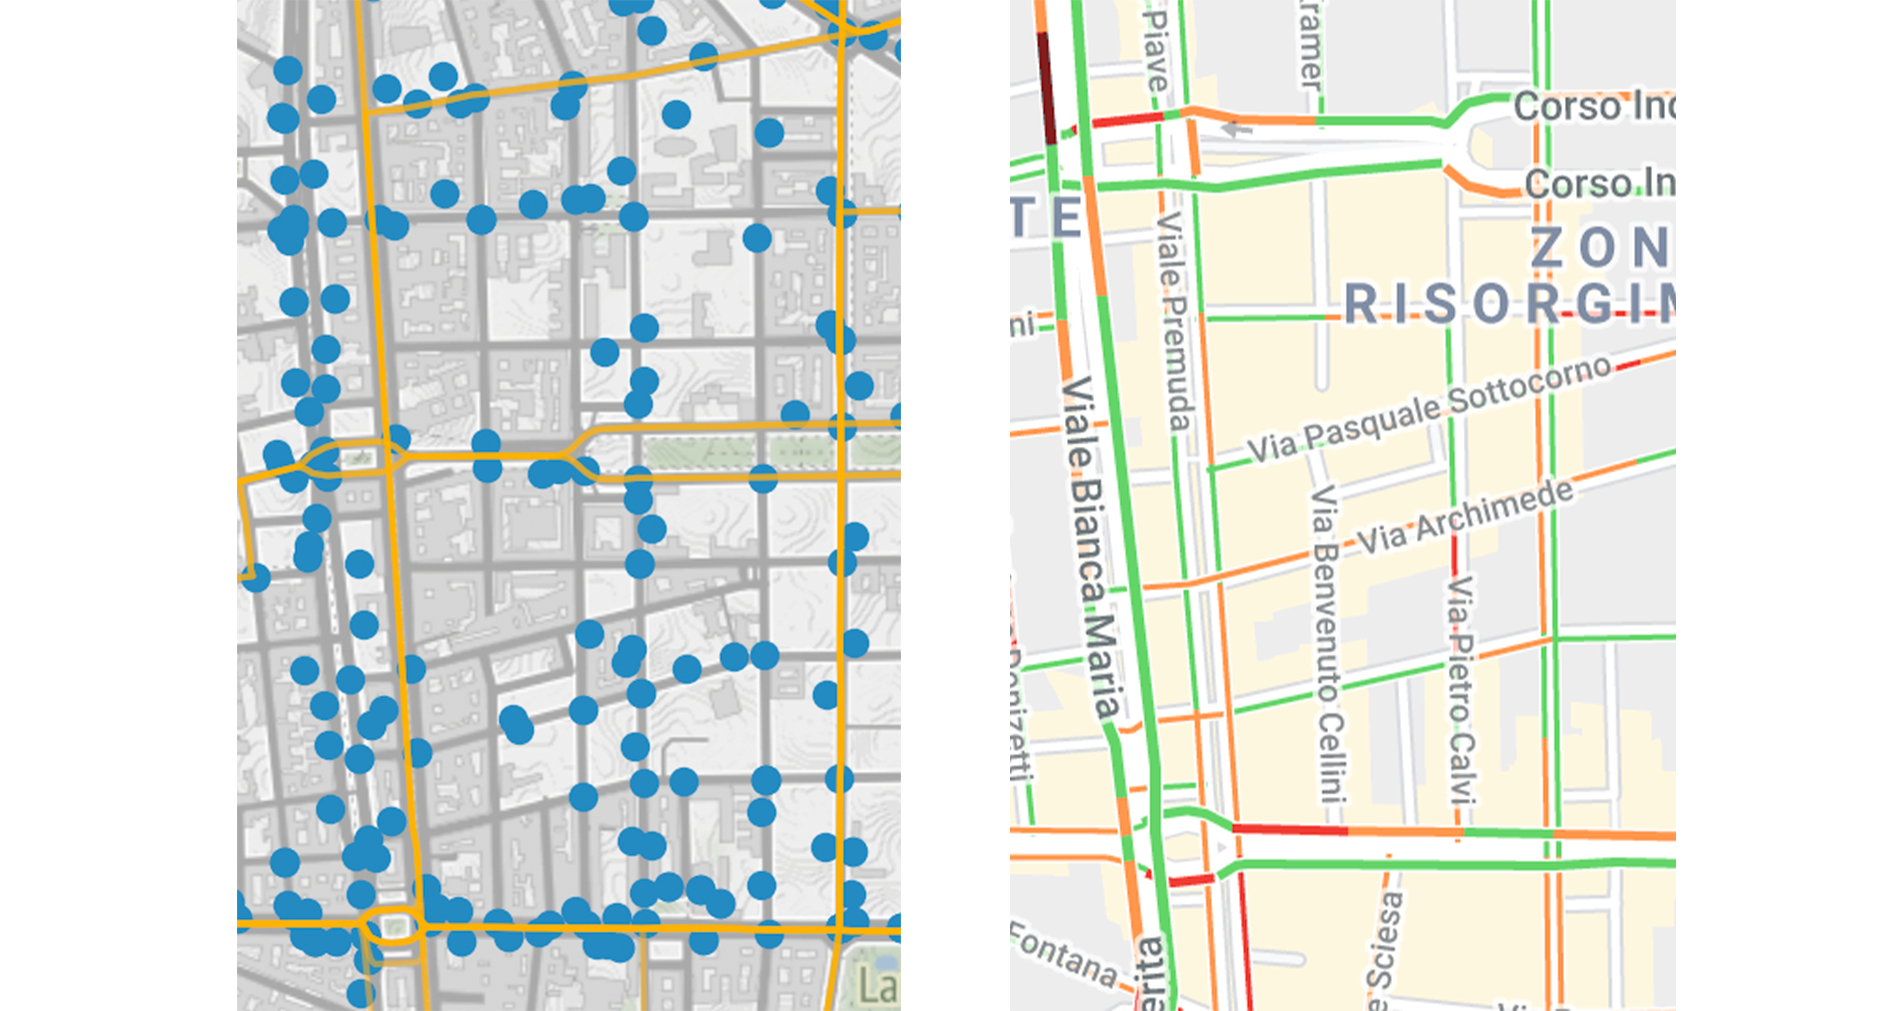
\includegraphics[width=\linewidth]{../src/atm/22_marzo.png}
    \caption{Linee dei trasporti pubblici e condizioni traffico vicino a Corso Ventidue Marzo}
    \label{fig:22-marzo}
\end{figure}

Le immagini del contenenti indicazioni sul traffico sono state realizzate tramite le API di 
Google Maps, tuttavia non offrono una stima ideale, poiche indicano il traffico in tempo reale e 
la quarantena per il Covid-19 ha ridotto notevolmente il volume di automobili.

Per confutare l'ipotesi iniziale, si sono utilizzati i dati ricavati in precedenza, 
cioè gli incindenti per chilometro per ogni municipio di Milano. 
Nella zona dei Navigli, si è poi presa in considerazione la sezione \ref{fig:zona-navigli-rect}, 
perchè sono presenti molti incidenti in viale Papiniano e viale Beatrice d'Este, 
e un numero minore nella vie parallele sottostanti, in cui sono anche presenti 
linee di trasporti pubblici.

\begin{figure}
    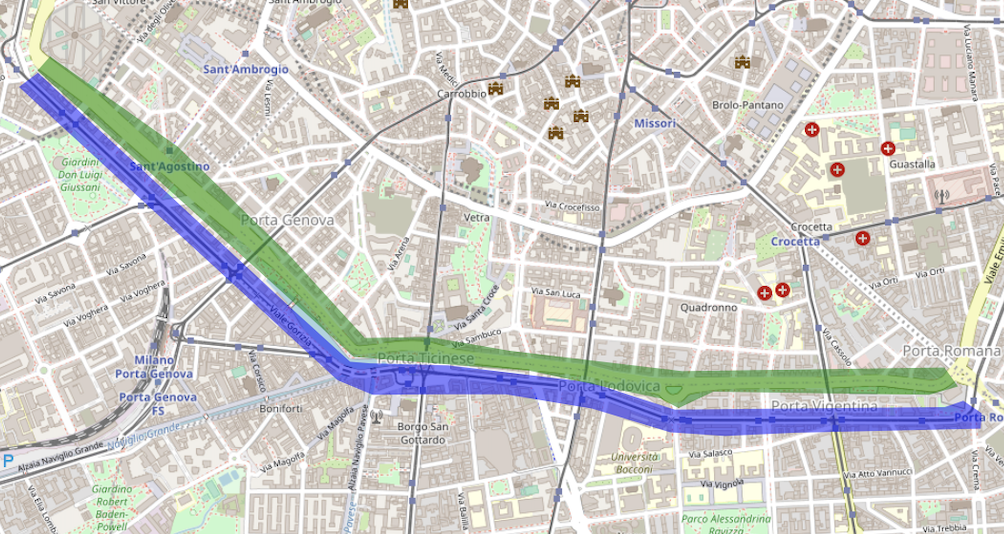
\includegraphics[width=\linewidth]{../src/atm/zona_navigli_rect.png}
    \caption{Sezioni di Milano prese in considerazione per contare gli incidenti ai Navigli}
    \label{fig:zona-navigli-rect}
\end{figure}

\begin{code}
data = gp.read_file("dataset/zone_milano/zone.geojson").to_crs(epsg=3857)
autobus = data[data['name'] == "Navigli Autobus"]
street = data[data['name'] == "Navigli Incidenti"]

autobus_rect = geometry.Polygon(autobus['geometry'].iloc[0])
street_rect = geometry.Polygon(street['geometry'].iloc[0])

inc_a = 0
inc_s = 0
for point in incidenti['geometry']: 
    point = geometry.Point(point)

    if autobus_rect.contains(point): 
        inc_a += 1
        
    if street_rect.contains(point): 
        inc_s += 1
\end{code}

Il risultato, conferma che avvengono $167.09$ incidenti per chilometro 
nel viale in cui sono presenti trasporti pubblici e, per quanto non sia nella media per la zona 
di appartenenza, è giustificabile in quanto si è presa in considerazione solo la strada, 
e non le \quotestyle{zone morte}.
Nell'altra via, invece, dove non passa alcuna linea di trasporti pubblici, 
gli incidenti sono $289.32$, risultato ancora più alto rispetto a quello ottenuto 
nella zona di Loreto. 

Non è detto che il maggior numero di incidenti sia causato dalla linea degli autobus, 
in particolare, va tenuta in considerazione la topologia delle due vie parallele.
La differenza principale tra Viale Bligny e Viale Beatrice d'Este è che, la prima è una via a due 
corsie per senso di marcia, mentre il secondo è un viale a due 
carreggiate\footnote{Carreggiata: la parte della strada destinata allo scorrimento dei veicoli, 
delimitata da una striscia continua o da un paracarro} 
con sensi di marcia separati da una zona non attraversabile da automobili. 
Dunque è ovvio che la maggior parte dei conducenti preferirà un viale ad alta velocità 
rispetto a una via dove è possibile rimanere incolonnati per la presenza di una sola 
corsia, e dove si è rallentati dalla presenza di autobus o tram.

Lo stesso procedimento è stato realizzato per Corso Ventidue Marzo, le zone utilizzate sono 
raffigurate nel'immagine \ref{fig:zona-22marzo-rect}. 

\begin{figure}
    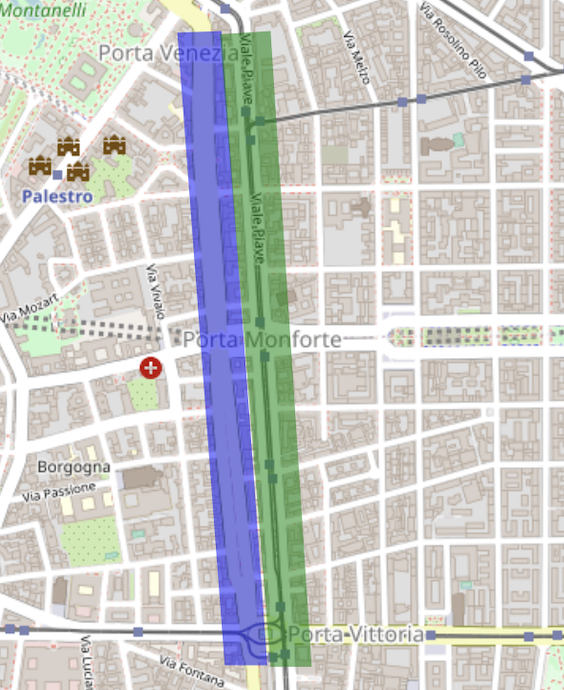
\includegraphics[width=\linewidth]{../src/atm/zona_22marzo_rect.png}
    \caption{Sezioni di Milano prese in considerazione per contare gli incidenti intorno a corso Ventidue Marzo}
    \label{fig:zona-22marzo-rect}
\end{figure}

In questo caso, per viale Bianca Maria, dove non è presente una linea di trasporti pubblici, 
il numero di incidenti è $254.31$, mentre per viale Premuda per cui passa una linea tranviaria, 
il numero scende a $93.96$.

Anche per questa zona, le due vie prese in considerazione sono molto diverse.
Viale Premuda è una via a due carreggiate separate, ognuna con una corsia e un solo senso 
di marcia, dove sono parcheggiate automobili su entambi i lati, e la velocità dei 
veicoli non deve essere particolarmente elevata.
Allo stesso modo, nel Viale Bianca Maria, le carreggiate sono separate, tuttavia queste 
hanno due, e in alcuni punti tre corsie ciascuna. 

Va sottolineato che le strade prese in considerazione hanno differenze sostanziali, e che 
probabilmente, il numero maggiore di incidenti su viali più ampi sia dovuto al 
volume di traffico più alto.
D'altro canto, è anche possibile che una parte dei conducenti, come quelli con più esperienza 
a giudare in grandi città, tengano in considerazione e evitino le strade con i mezzi pubblici.

%\clearpage
\subsection{Il pavè a Milano influisce in qualche modo sull'incidentalità?}

Nella sezione sull'origine dei dati, si è parlato di come è stato possibile ricavare 
un tracciato con la maggior parte delle strade in pavè a Milano.

Per valutare le somiglianze tra le linee tranviarie e la cartina di 
Urbanfile, si è utilizzata l'immagine \ref{fig:tram-pave-milano}.

\begin{figure}
    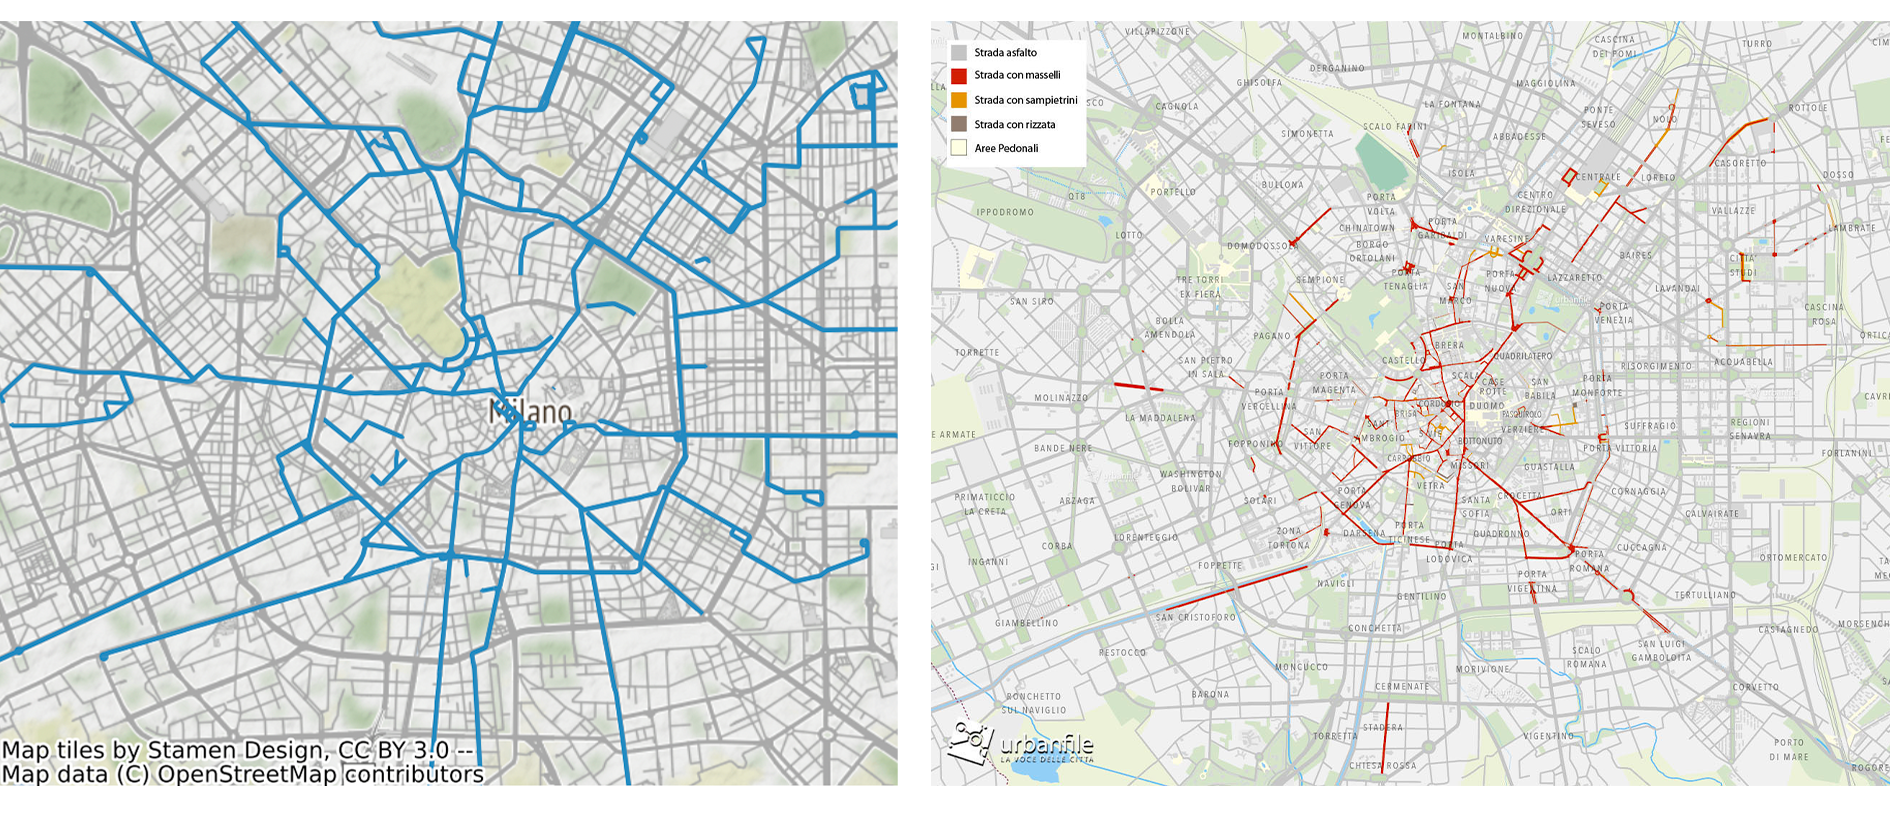
\includegraphics[width=\linewidth]{../src/tram/tram_milano.png}
    \caption{Cartina con strade in pavè e linee tranviarie a Milano}
    \label{fig:tram-pave-milano}
\end{figure}

\'E possibile notare alcune somiglianze, come per esempio viale Sabotino e via 
Alessandro Mazoni, tuttavia la maggior parte delle linee tranviarie segnate 
passano su asfalto.
Inoltre, in alcuni viali, come viale Premuda, i tram hanno una carreggiata separata, 
che molto probabilmente ha influenza ancora minore sugli incidenti della zona.

Viste le basse somiglianze tra la cartina di Urbanfile e le linee del tram, 
per creare una stima, si sono convertite le vie principali della mappa trovata 
in geojson. 
Il risultato è visibile nella mappa sulla sinistra dell'immagine \ref{fig:mappa-pave}.

\begin{figure}
    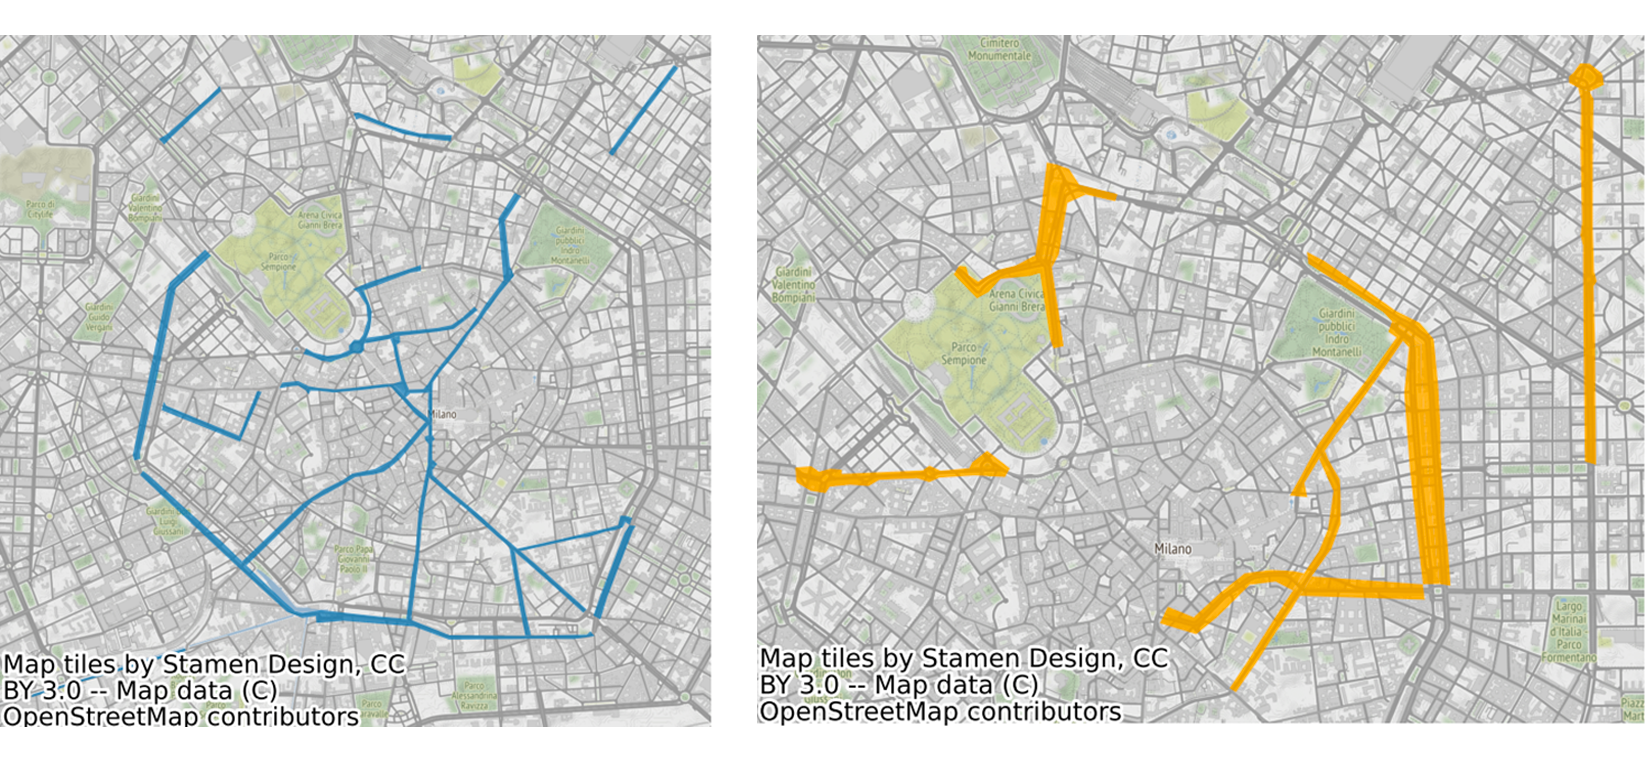
\includegraphics[width=\linewidth]{img_unite/mappa_pave_asfalto.png}
    \caption{Principali strade a Milano in pavè e campione simile di strade asfaltate}
    \label{fig:mappa-pave}
\end{figure}

Una volta creata l'area delle strade in pavè, è possibile calcolare quanti sono gli 
incidenti che avvengono in queste zone e confrontarlo con il numero di incidenti 
nelle strade asfaltate.

\begin{code}
inc_in_pave = 0
for rect in pave['geometry']: 
    rect = geometry.Polygon(rect)

    for point in incidenti['geometry']: 
        if rect.contains(geometry.Point(point)): 
            inc_in_pave += 1

area_pave = 0
for rect in pave['geometry']: 
    area_pave += geometry.Polygon(rect).area

incidenti_per_km = inc_in_pave * 10**6 / area_pave
\end{code}

Il numero di incidenti per chilometro quadrato, nelle strade in pavè è $229.45$, che 
è un valore particolarmente alto, anche se viene confrontato con il numero di 
incidenti nel centro storico, cioè circa $130$.
Tuttavia, bisogna tenere in considerazione che il dataset che è appena stato creato, 
contiene solamente strade, senza alcuna zona morta, come edifici, mentre l'area utilizzata 
del centro storico, contiene tutto il territorio del centro.

Per ovviare a questo problema, si è creato un campione di strade asfaltate, prese circa 
nella stessa zona di Milano. 
Queste strade sono raffigurate nella mappa destra in figura \ref{fig:mappa-pave}. 
Si è tentato di aggiungere al campione strade più simili possibili a 
quelle in pavè, sia per zona, sia per topologia. 
Inoltre, per lo stesso motivo, l'area totale dei due dataset è simile.

Eseguendo lo stesso calcolo realizzato per le strade in pavè, risulta che il numero di incidenti per 
chilometro quadrato, nel campione creato, sia di $220.89$ incidenti.
Tuttavia, nel campione delle strade asfaltate sono stati presi vari tratti provenienti dalla 
circonvallazione interna e altre zone molto trafficate, mentre il campione di strade in pavè 
contiene, per mancanza di altri dati, molte strade del centro storico, inevitabilmente 
meno trafficate.

%\clearpage
\section{Incidenti e Autovelox}

Per sapere se gli autovelox hanno influenza sull'incidentalità, 
bisognerebbe innanzi tutto sapere quando sono stati posizionati i dispositivi, e solo 
a quel punto, avendo dati su incidenti prima e dopo l'installazione, sarebbe 
possibile trarre conclusioni.

Alcuni dati sull'installazione di autovelox esistono per l'anno 2014, visualizzabili 
nella tabella \ref{ztl-milano}, tuttavia le posizioni degli incidenti 
sono solo disponibili per l'anno 2016, in quanto Istat non ha rilasciato 
le posizioni precise degli incidenti in altre annate.

Conoscendo il nome della via degli autovelox installati nel 2014, è possibile ricondursi 
alla posizione effettiva di questi ultimi sulla mappa.
Per fare ciò, la soluzione più veloce è stata quella di enumerare tutti gli autovelox, 
e confrontarli con le vie della tabella, salvando le posizioni che coincidono.
Il risultato è rappresentato nella mappa sul lato sinistro della 
figura \ref{fig:autovelox-indici}.

\begin{code}[language=Python]
path = "dataset/autovelox/autovelox_milano.geojson"
autovelox = gp.read_file(path).to_crs(epsg=3857)
layer_autovelox = autovelox.plot(figsize=(11,9), color="red")
    
index = 0
for lat, lon in geo_utils.parse_geojson_point_list(autovelox['geometry'].astype(str)):
    layer_autovelox.text(lat, lon, s=index)
    # si aggiunge un label per ogni punto
    index += 1
    
cx.add_basemap(ax=layer_autovelox)
plt.show()
\end{code}

\begin{figure}
    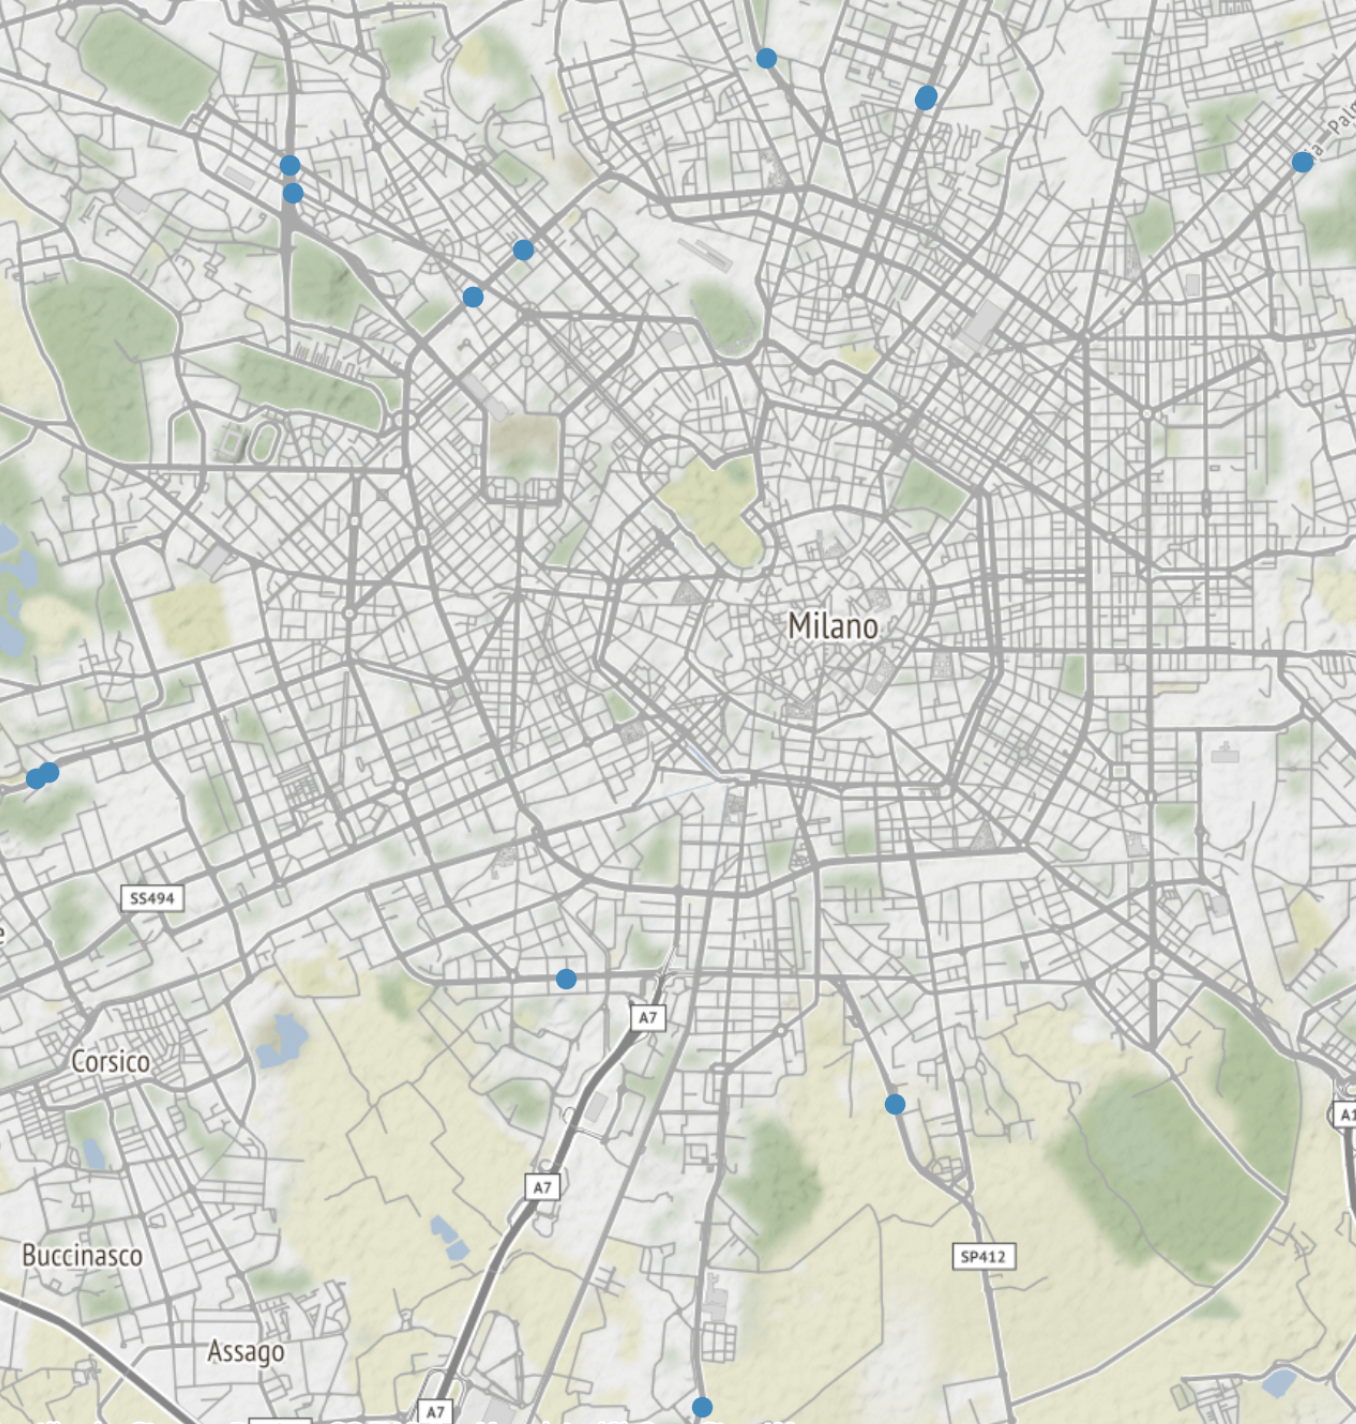
\includegraphics[width=\linewidth]{../src/autovelox/autovelox_2014.png}
    \caption{Autovelox installati nel 2014 e quelli il cui anno di installazione è ignoto}
    \label{fig:autovelox-indici}
\end{figure}

Per quanto non si disponga delle informazioni sugli incidenti prima e dopo dell'installazione, 
è comunque possibile sovrapporre i dataset, per vedere se gli autovelox hanno un qualche tipo di 
effetto sugli incidenti, visto che i dati sui sinistri sono successivi all'installazione 
delle telecamere.

\begin{figure}
    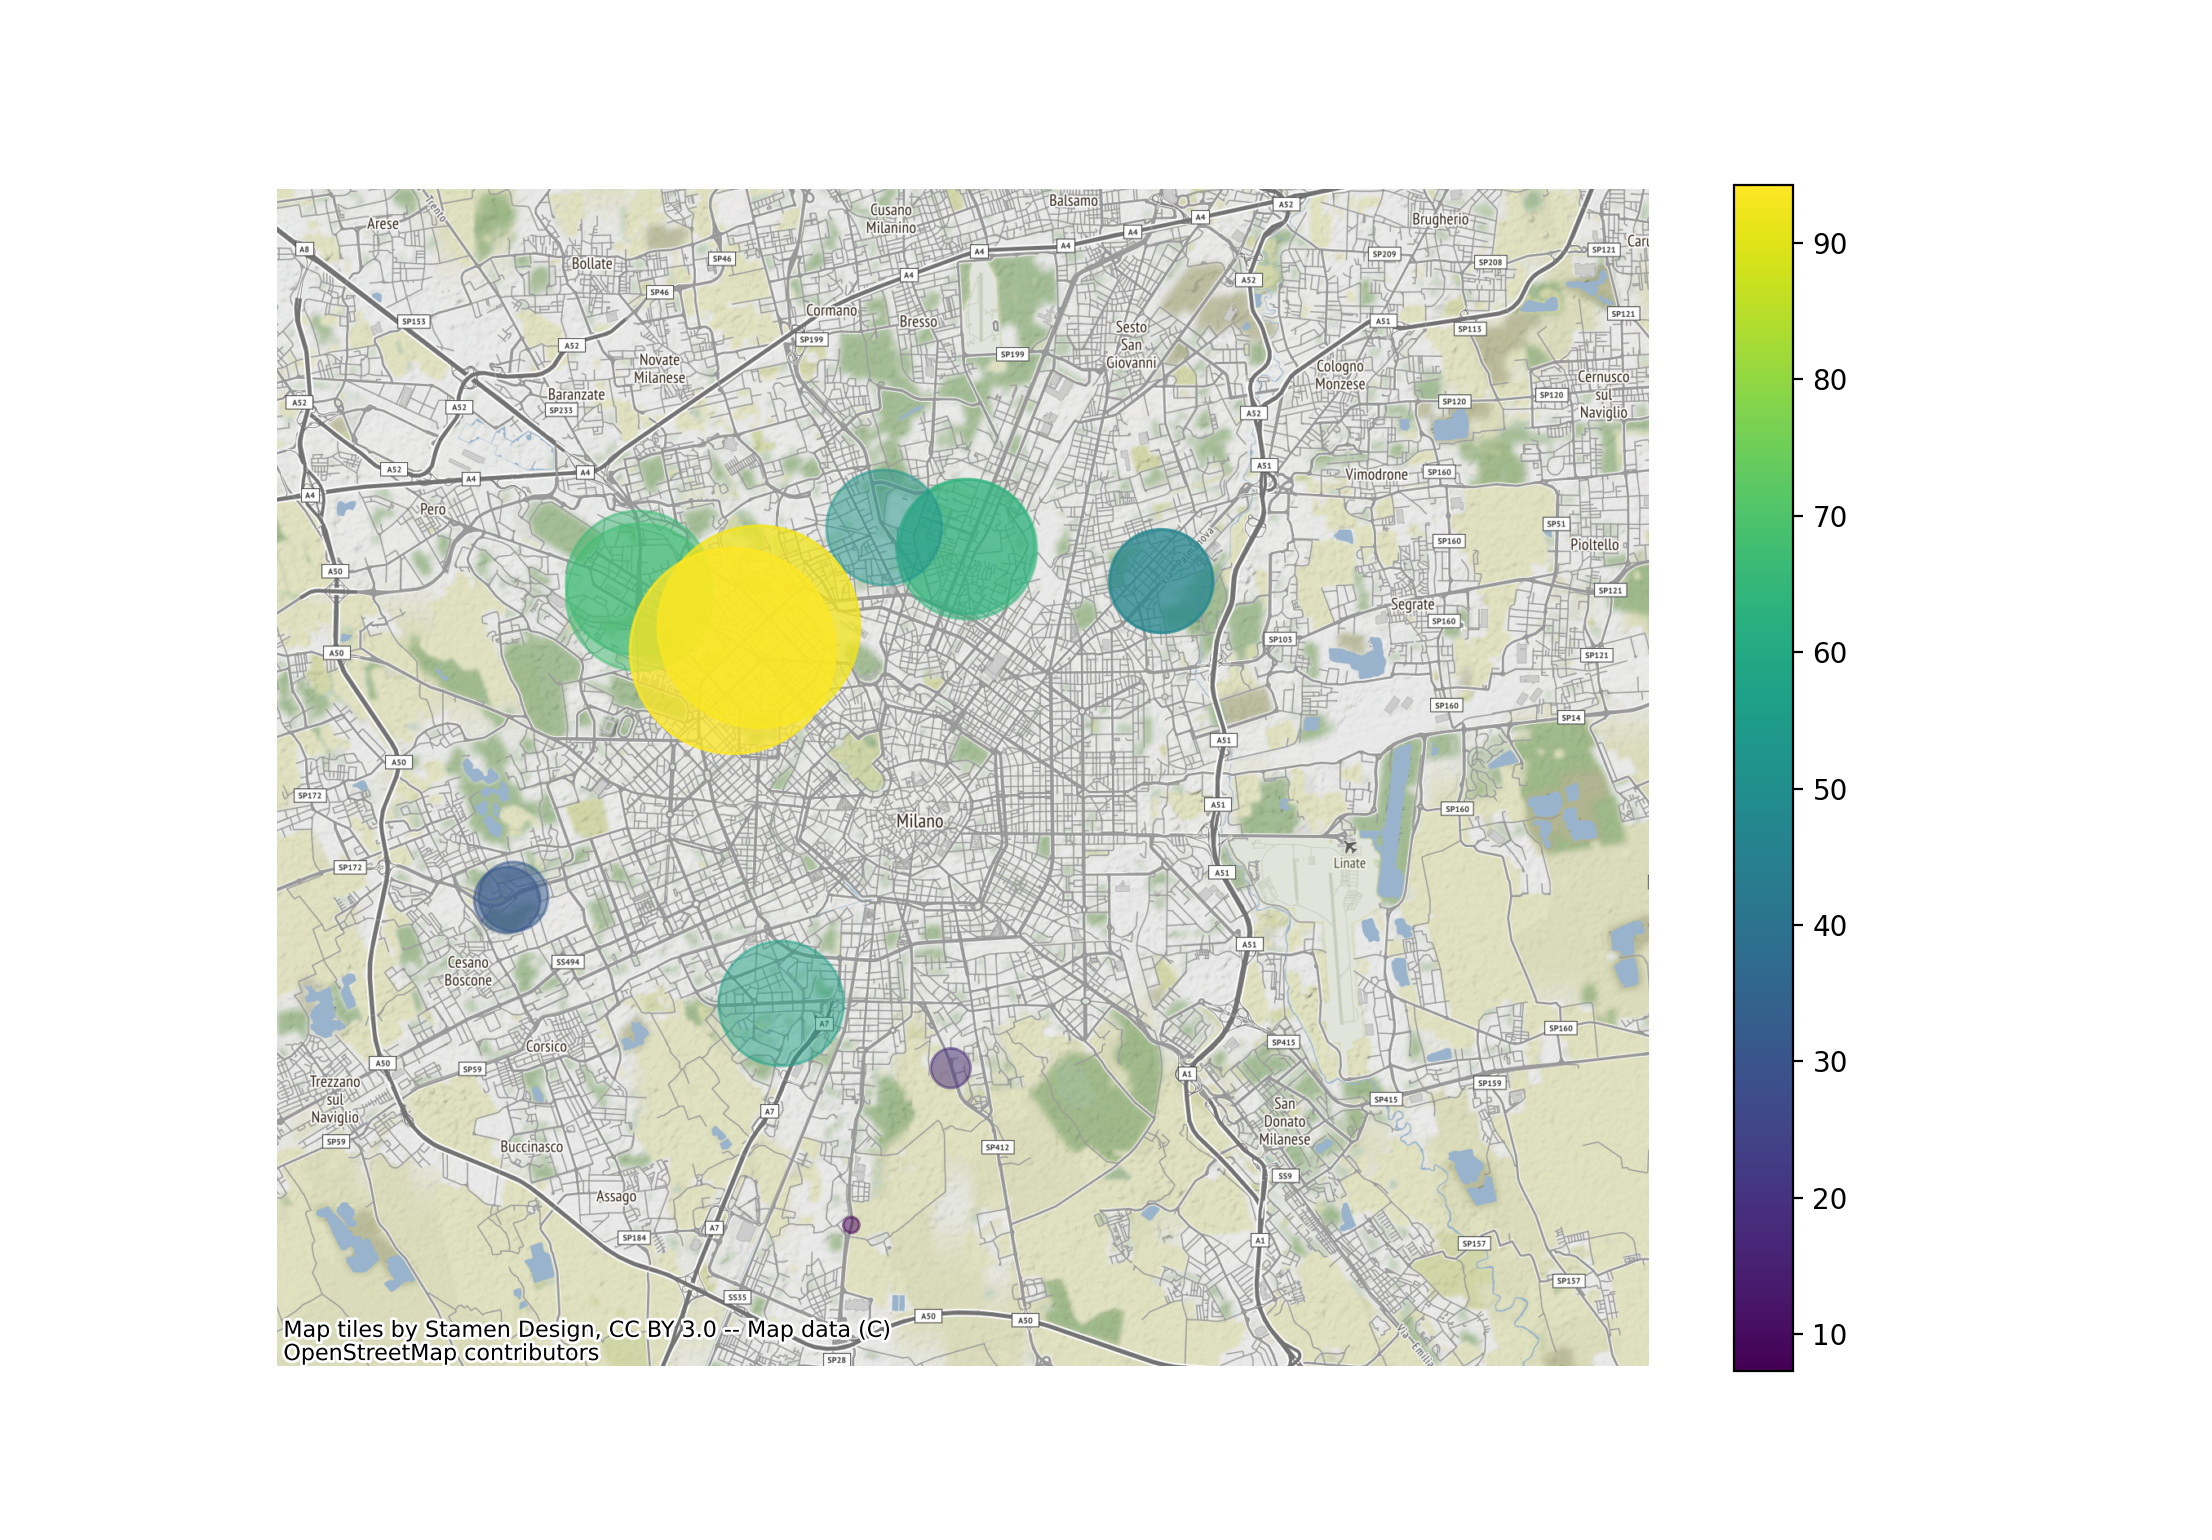
\includegraphics[width=\linewidth]{../src/autovelox/autovelox_incidenti.png}
    \caption{Autovelox e Incidenti a Milano}
    \label{fig:autovelox-incidenti}
\end{figure}

La mappa \ref{fig:autovelox-incidenti} è stata realizzata contando gli incidenti avvenuti 
nel raggio di un chilometro a ogni autovelox, in quanto non si dispone del nome della 
via nel quale è avvenuto il sinistro. 
Va precisato che le \quotestyle{bolle} non indicano il raggio di conteggio degli incidenti, ma 
il numero dei sinistri trovati. La colorazione dei \quotestyle{cerchi} è stata aggiunta per 
rendere il grafo più leggibile, la cui interpretazione poteva essere difficoltosa 
osservando solo l'ampiezza del raggio di questi.

\begin{center}
    \def\arraystretch{1.5}% 
    \begin{tabular}{ |c|c|c|c| }
        \hline
        Autovelox & Inc. Totali & Inc. per $Km^2$ & Inc. per zona \\ 
        \hline
        \rowcolor{TableGray}
        V. F. Testi d. perif.\footnotemark[1]   &   194 &   61.78   &   69.52 \\
        V. F. Testi d. centro                   &   202 &   64.33   &   69.52 \\
        \rowcolor{TableGray}
        C. Ghisallo d. centro\footnotemark[2]   &   208 &   66.24   &   44.3 \\
        C. Ghisallo d. perif.                   &   212 &   67.51   &   44.3 \\
        \rowcolor{TableGray}
        V. Fermi                                &   166 &   52.86   &   51.25 \\
        V. Parri d. perif.                      &    95 &   30.25   &   43.63 \\
        \rowcolor{TableGray}
        V. Parri d. centro                      &   100 &   31.84   &   43.63 \\
        V. Famagosta                            &   180 &   57.32   &   43.63 \\
        \rowcolor{TableGray}
        V. Missaglia d. centro                  &   23  &    7.32   &   27.54 \\
        V. Ferrari                              &   57  &   18.15   &   44.3 \\
        \rowcolor{TableGray}
        V. Monteceneri d. Serra                 &   291 &   92.67   &   44.3 \\
        V. Monteceneri d. Lugano                &   290 &   92.35   &   44.3 \\
        \rowcolor{TableGray}
        Viale Serra                             &   296 &   94.26   &   44.3 \\
        Viale Serra                             &   296 &   94.26   &   44.3 \\
        \rowcolor{TableGray}
        V. Palmanova d. perif.                  &   149 &   47.45   &   59.79 \\
        V. Palmanova d. centro                  &   149 &   47.45   &   59.79 \\
        \hline
    \end{tabular}
\end{center}

\footnotetext[1]{Viale Fulvio Testi}
\footnotetext[2]{Cavalcavia del Ghisallo}

Una volta trovati gli incidenti totali, è possile calcolare il numero di sinistri 
sulla base dell'area utilizzata.
Al dataset degli autovelox sono aggiunte due colonne, una contenente gli incidenti totali, 
l'altra contenente gli incidenti per chilometro.

\begin{code}
autovelox_2014['incidenti_vicini'] = gp.GeoSeries(df)
autovelox_2014['incidenti_pesati'] = autovelox_2014['incidenti_vicini'] / 3.14
\end{code}

Questa ultima colonna, in particolare, è divisa per 3.14 perchè l'area del cerchio 
è data dalla formula: 

\begin{center}
    $Area\, = \pi * r^2$
\end{center}

E, poichè si sta utilizzando un raggio di circa un chilometro, e si vuole ottenere il 
numero di incidenti per chilometro quadrato, l'area ottentuta è $3.14$.

Per facilitare la lettura della tabella precedente, nella figura \ref{fig:confronto-autovelox} 
è visibile il confronto tra il numero di incidenti vicino a autovelox, e il numero di incidenti 
del municipio.
In alcuni casi, il numero di incidenti sembra essere ridotto dalla presenza della telecamera,  
tuttavia nella maggior parte dei casi, e soprattutto nelle zone di Viale Serra e 
Viale Monteceneri, il volume di incidenti è particolarmente più alto di 
quello della zona municipale.

\begin{figure}
    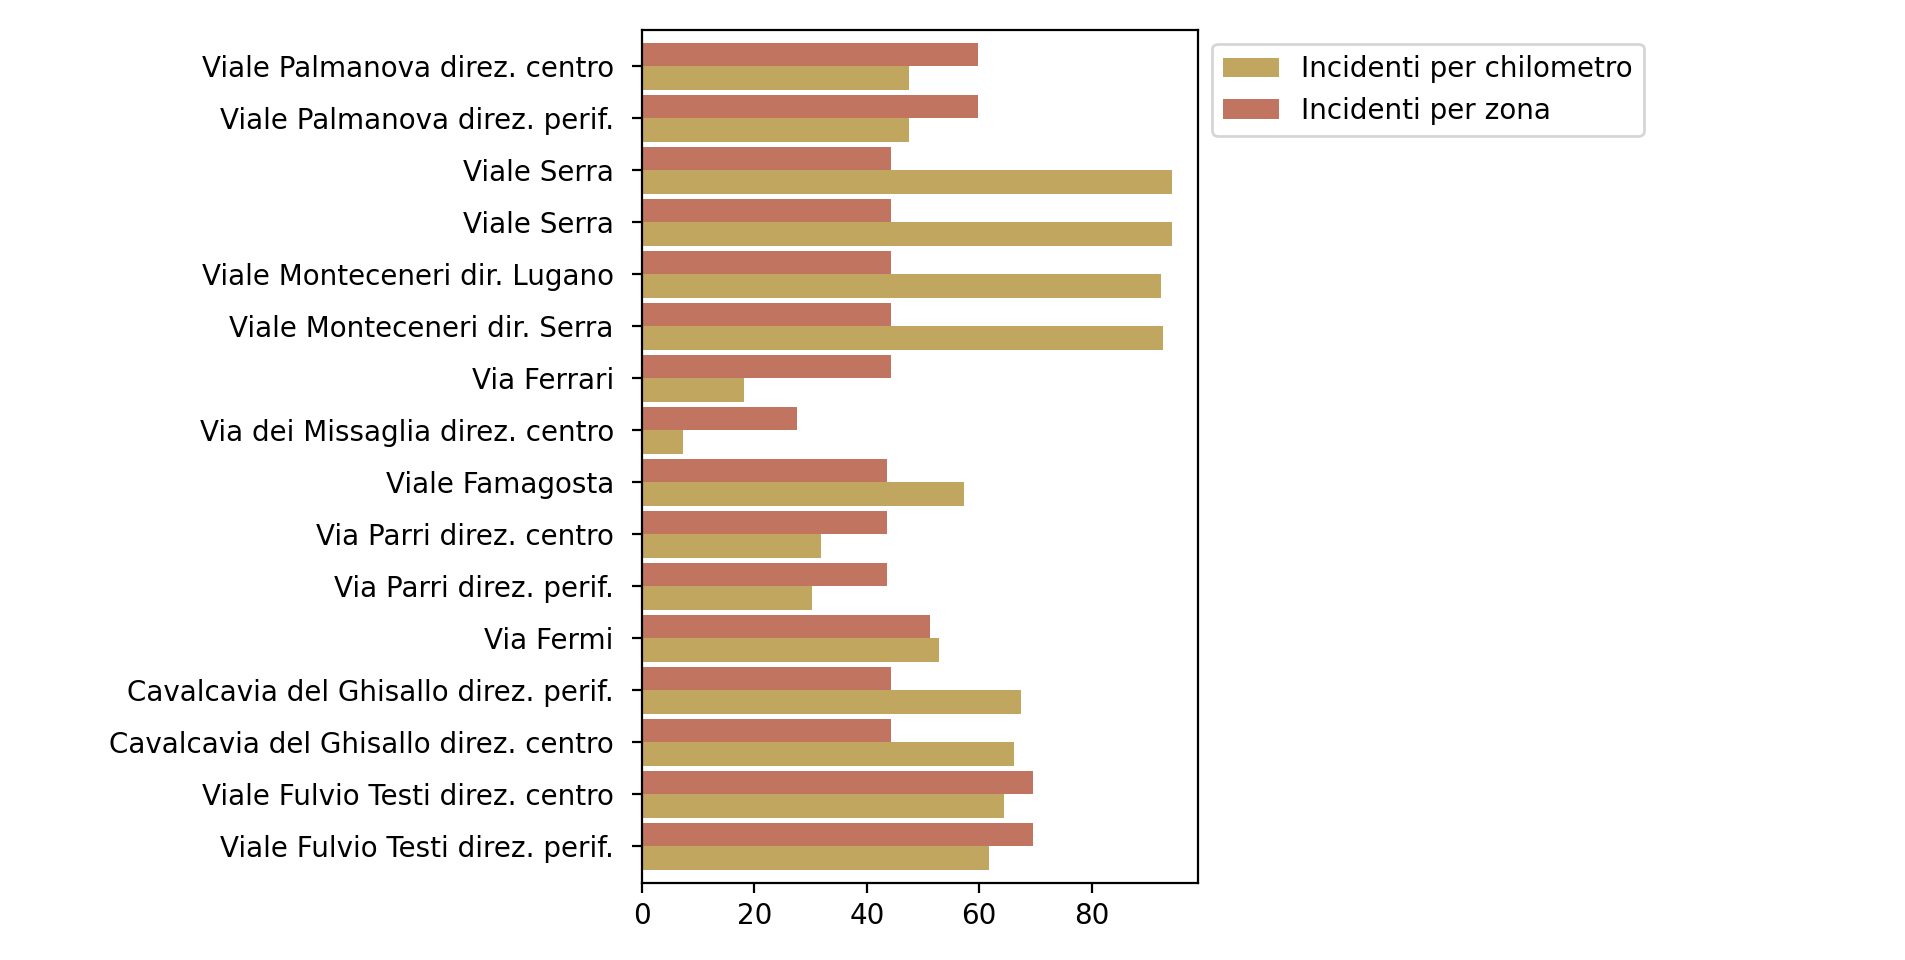
\includegraphics[width=\linewidth]{../src/municipi_milano/conclusioni_municipio.png}
    \caption{Incidenti vicino a autovelox rispetto a quelli per zona di Milano}
    \label{fig:confronto-autovelox}
\end{figure}

\begin{code}
incremento_percentuale_totale = 0
for km, zona in zip(data['Incidenti per chilometro'], data['Incidenti per zona']): 
    incremento_percentuale = (km - zona) * 100 / zona
    incremento_percentuale_totale += incremento_percentuale

print(incremento_percentuale_totale)
\end{code}

Sarebbe interessante \quotestyle{catturare}, in un solo valore, l'incremento (o decremento) 
globale, degli incidenti in zone vicine a 
autovelox\footnote{Si tenta di capire, con un solo numero, se la presenza di autovelox nella zona 
aumenta o diminuisce il numero di sinistri}.
A causa delle zone menzionate in precedenza, in vicinanza di autovelox si ha un incremento degli 
incidenti del $329.6$\%, tuttavia, nel caso in cui si considerino 
outlier\footnote{In un campione di osservazioni, un outlier è un valore anomalo, 
particolarmente distante dagli altri dati disponibili \cite{PROB_E_STATISTICA:1}} 
i Viali Serra e Monteceneri, si ha invece un decremento generale del $113.6$\%.

Va comunque sottolineato che, non avendo dati sufficienti a calcolare una tendenza 
precedente all'installazione dell'autovelox, non si ha modo di sapere se questi abbiano un 
effetto positivo o negativo sull'incidentalità.
Con il rilascio di nuovi dataset di incidenti geolocalizzati, possibilmente riferiti ad annate 
precedenti al 2014, sarebbe possibile realizzare una stima con informazioni antecedenti e 
successive all'installazione delle telecamere.


%%%%%%%%%%%%%%%%%%%%%%%%%%%%%%%%%%%%%%%%%%%%%%%%%%%%%%
%\clearpage
\chapter{Dati su Incidenti}

Per quanto riguarda i dati sugli incidenti in Italia, sono disponibili due dataset 
molto ampi. 
Il primo, rilasciato da Istat, contiene campi come data, ora, 
numero di persone a bordo, tipo di incrocio e tipo di veicolo.
Queste informazioni sono presenti a partire dal 2010 fino al 2018.
Il secondo è invece messo a disposizione da Automobile Club D'Italia (ACI) che contiene dati simili, 
e in più informazioni sul luogo dell'incidente, come autostrada o strada provinciale, 
inteso come il nome della strada, il che permette di avere una minima localizzazione del 
sinistro.

%\clearpage
\section{Dati Istat su veicoli}

%\clearpage
\subsection{Il tipo di veicolo dipende dalla strada?}

Una prima analisi che è possibile realizzare, è, per quanto riguarda i veicoli, come 
la composizione di questi cambia al cambiare del tipo di strada. 
In altre parole, la percentuale, per esempio, di autotreni nelle autostrade, è diversa rispetto 
a quella nelle strade provinciali? 

\begin{code}[language=Python]
# Dove 1,2,3 sono gli ID dei diversi tipi di strade urbane, 
# mentre 4,5,6 gli ID delle strade extraurbane

strade_urbane = data[(data['localizzazione_incidente'] == 1) | (data['localizzazione_incidente'] == 2) | (data['localizzazione_incidente'] == 3)]['tipo_veicolo_a']
strade_extraurbane = data[(data['localizzazione_incidente'] == 4) | (data['localizzazione_incidente'] == 5) | (data['localizzazione_incidente'] == 6)]['tipo_veicolo_a']
\end{code}

Il grafo \ref{fig:differenza-strade} rappresenta quali sono le categorie di veicoli 
coinvolte con più frequenza in sinistri, per tre tipi di strade diverse, strade urbane, 
extraurbane e autostrade. 
Le percentuali sono calcolate per gruppo, quindi sommando 
tutte le righe di, per esempio \columnstyle{Autostrade}, si ottiene $1.0$.

\begin{figure}
    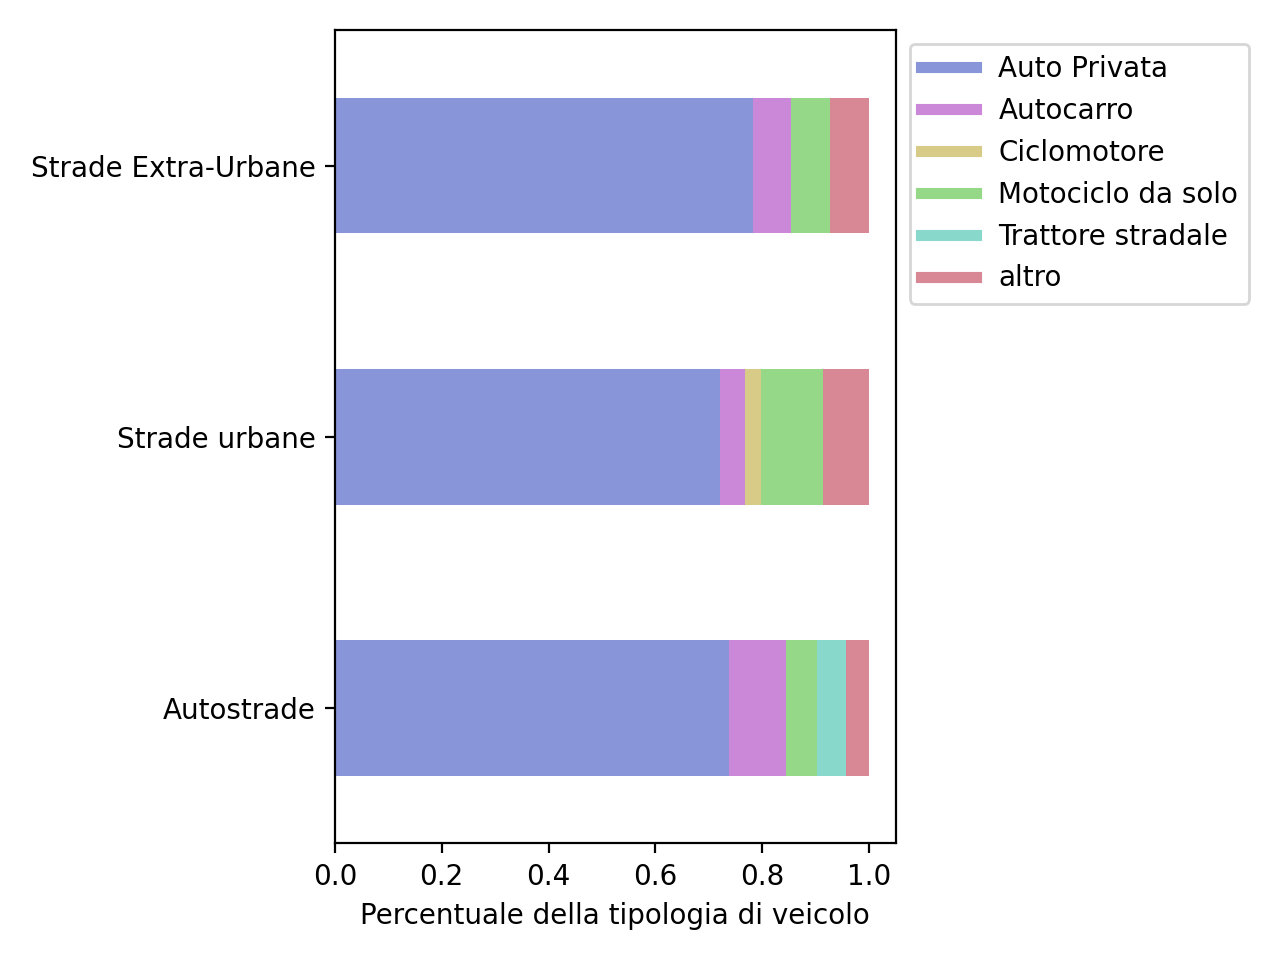
\includegraphics[width=\linewidth]{../src/incidenti/incidenti_senza_coords/tipo_veicoli/differenza_strade.png}
    \caption{Incidenti per tipo di veicolo nel 2018}
    \label{fig:differenza-strade}
\end{figure}

Nonostante le auto private siano di gran lunga il tipo di veicolo 
più coinvolto in incidenti, nelle autostrade non sono presenti molti incidenti con motocicli, 
mentre cresce molto il numero di questi nelle strade urbane.
Nel caso degli autotreni, si ha invece una bassa percentuale di questi nelle strade 
urbane, mentre il numero si alza nelle autostrade.

Visto che le auto private causano oltre tre quarti degli incidenti in ogni categoria di strada,  
si è deciso di ometterle, per controllare la presenza di differenze nelle altre tipologie 
di veicoli.
I risultati sono rappresentati, per l'anno 2018, nella figura \ref{fig:differenza-strade-no-auto}.

\begin{figure}
    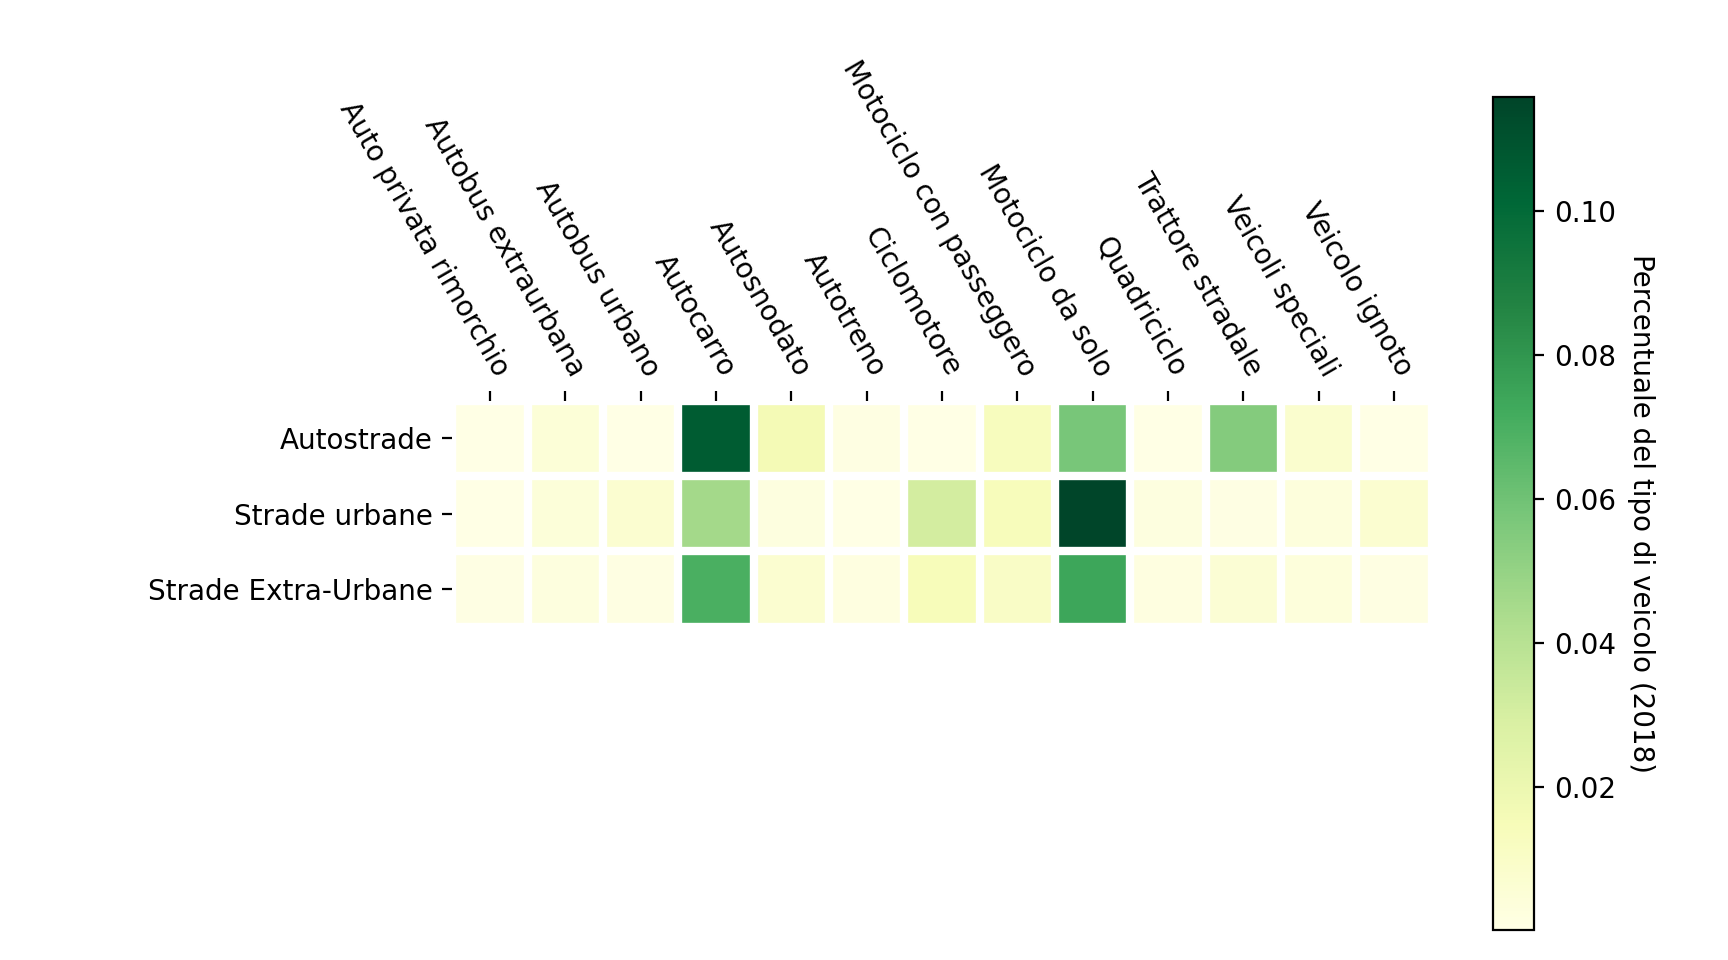
\includegraphics[width=\linewidth]{../src/incidenti/incidenti_senza_coords/tipo_veicoli/differenza_senza_auto.png}
    \caption{Incidenti per tipo veicolo, senza contare le auto private}
    \label{fig:differenza-strade-no-auto}
\end{figure}

Omesse le automobili private, appare chiaro che gli autocarri siano coinvolti in un maggior 
numero di incidenti su autostrade, mentre i motocicli abbiano il primato sulle strade urbane.
Può anche sembrare strano che i trattori stradali siano coinvolti così spesso in incidenti 
su autostrade, tuttavia, in questo caso, per \quotestyle{trattore} non si intende la macchina 
agricola, ma la motrice di un autocarro senza rimorchio.

Va comunque sottolineato che le percentuali di incidenti provocati da queste tipologie di 
veicoli, sono tutte al di sotto del $10$\%, e che la sezione più ingente di sinistri è 
provocata dalle automobili private. 
Inoltre, utilizzare il numero di incidenti come stimatore\footnote{Stimatore: una qualunque statistica con 
lo scopo di dare una stima di un parametro $\theta$ è detta stimatore 
di $\theta$ \cite{PROB_E_STATISTICA:4}} 
del traffico, potrebbe non portare a un risultato ottimale. 

%\clearpage
\section{Dati Istat su conducenti e passeggeri}

%\clearpage
\subsection{Esistono differenze tra la guida di un uomo e quella di una donna?}

Un frequente stereotipo infondato riguardante le donne alla guida, è che queste 
ultime siano meno abili rispetto a individui del sesso opposto. 
Avendo a disposizione le informazioni sul sesso del conducente che ha causato l'incidente, 
è possibile controllare se esista un riscontro reale per questa ipotesi.

\begin{figure}
    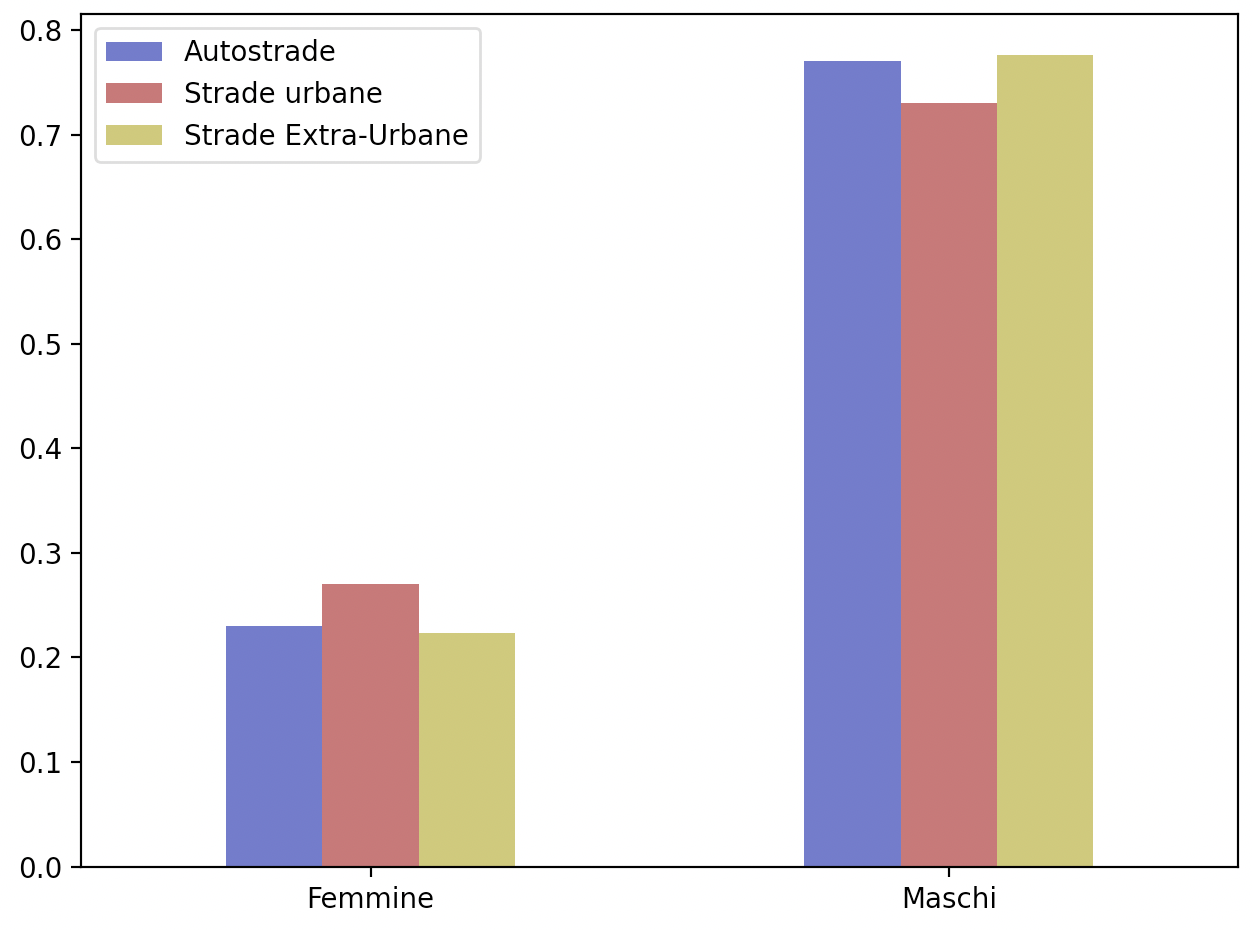
\includegraphics[width=\linewidth]{../src/incidenti/incidenti_senza_coords/tipo_veicoli/uomo-donna.png}
    \caption{Sesso del conducente per tipo di veicolo nel 2018}
    \label{fig:differenza-uomo-donna}
\end{figure}

Il grafo \ref{fig:differenza-uomo-donna} mostra le percentuali di incidenti causate 
da uomini e donne, per tre diverse tipologie di strada. 
Per quanto riguarda il tipo di strada, non è possibile individuare una 
variazione nella percentuale di incidenti così ingente. 
La variazione più ampia si registra sulle strade urbane, dove le donne causano circa il 
$5$\% di incidenti in più, nonostante ciò il numero 
di incidenti per genere tende ad essere causato per il $75$\% circa da uomini e 
per il $25$\% donne.

Avendo a disposizione i dati provenienti da tutte le annate a partire dal 2010, 
è anche possibile controllare se le percentuali trovate siano costanti al 
passare del tempo.
Nella tabella sottostante sono state riportate le stesse percentuali per le 
autostrade e le strade urbane.

\begin{center}
    \def\arraystretch{1.5}% 
    \begin{tabular}{ |c|c|c|c| }
        \hline
        Anno & Sesso & Autostrade & Strade Urbane \\ 
        \hline
        \rowcolor{TableGray}
        2018 & Uomo & 77\%  & 73\% \\
        2018 & Donna & 23\% & 27\% \\
        \rowcolor{TableGray}
        2016 & Uomo & 75.8\%  & 71.9\% \\
        2016 & Donna & 24.2\% & 28.1\% \\
        \rowcolor{TableGray}
        2014 & Uomo & 74.2\%  & 70.7\% \\
        2014 & Donna & 25.8\% & 29.3\% \\
        \hline
    \end{tabular}
\end{center}

In tutti gli anni la percentuale di uomini e donne coinvolti in incidenti è consistente, 
questo fenomeno fa sospettare che ci siano più uomini al volante rispetto alle donne.
Un modo per testare l'ipotesi è quello di ricavare un campione di conducenti, 
separando tra uomini e donne.
Va sottolineato che un campione, preso durante la pandemia di Covid-19, in un 
mese di quarantena non sarà mai uno stimatore estremamente accurato della percentuale 
di maschi e femmine al volante.

Si sono comunque contati i conducenti delle vetture passanti a Somma 
Lombardo\footnote{sul Sempione basso, strada urbana principale, all'altezza 
chiesa di San Bernardino}, 
tra le 15 e le 16 di Giovedì 5 Novembre 
(settimana predente alla seconda chiusura della Lombardia), 
sono stati ottenuti i seguenti risultati:

\begin{center}
    \def\arraystretch{1.5}% 
    \begin{tabular}{ |c|c|c| }
        \hline
        Sesso & Numero & Percentuale \\ 
        \hline
        \rowcolor{TableGray}
        Uomini & 483 & 68.8\% \\
        Donne & 219 & 31.2\% \\
        \hline
    \end{tabular}
\end{center}

La percentuale di uomini e donne al volante è equivalente a quella degli incidenti.
Questo dato rafforza l'idea che non esistano differenze sostanziali tra la guida di 
maschi e femmine, in quanto, assumendo che la probabilità che una donna causi un 
incidente sia uguale a quella di un uomo, le percentuali che si otterrebbero sarebbero 
le stesse del campione.

%\clearpage
\subsection{Il numero di passeggeri influisce sull'incidentalità?}

Il dataset Istat dispone anche di una serie di colonne corrispondenti all'età, sesso e 
all'esito di tre passeggeri, oltre al conducente.
Con un po' di lavoro, è possibile ricavare quanti passeggeri sono presenti 
nell'automobile al momento dell'incidente, in modo da controllare se esista una 
relazione tra numero di persone nella macchina e l'incidentalità.

\begin{figure}
    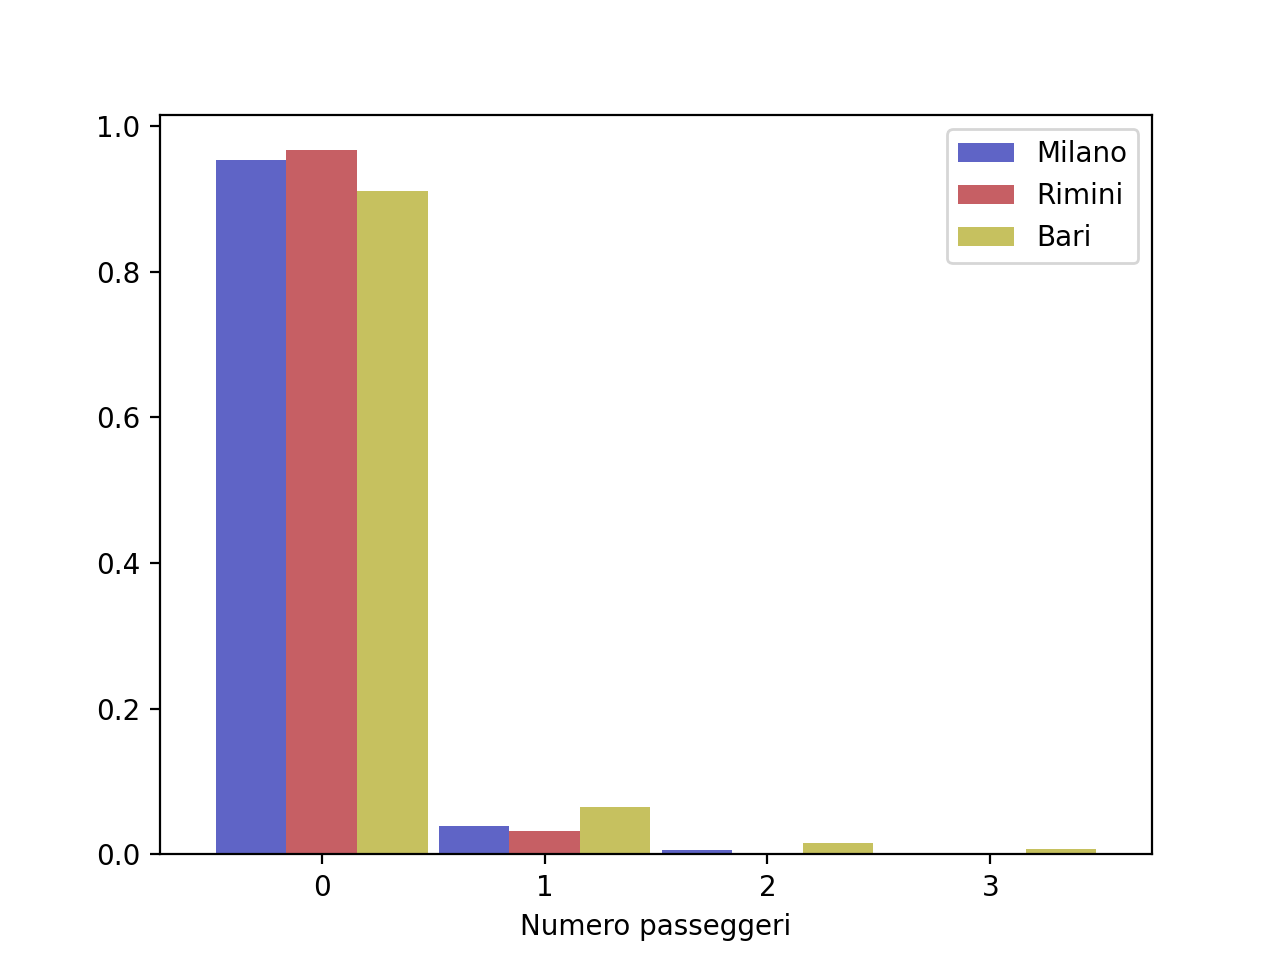
\includegraphics[width=\linewidth]{../src/incidenti/incidenti_senza_coords/passeggeri/passeggeri.png}
    \caption{Numero di passeggeri in incidenti per Milano, Rimini e Bari}
    \label{fig:passeggeri-milano-rimini}
\end{figure}

La figura \ref{fig:passeggeri-milano-rimini} mostra che oltre il 90\% degli incidenti
avviene quando in macchina è presente solo il conducente, cioè la colonna indicata con 0.
Si sono prese in considerazione le provincie di Milano, Rimini e Bari, 
per controllare se la località marittima influisse sul numero di incidenti.
Non sembra, tuttavia, esserci una grande differenza tra le province, con Rimini dove è 
più alto il numero di incidenti con solo il conducente, mentre a Bari vale l'opposto.

La domanda che sorge spontanea, dunque, è se avvengano più incidenti dove è presente 
solo il conducente per il numero frequente di automobili con una sola persona a 
bordo, o se esistano fattori esterni che portano il conducente a distrarsi?

Sarebbe utile poter ricavare un campione di automobili divise per 
numero di persone a bordo, tuttavia, in periodo di Covid-19, una stima di questo tipo 
non sarà mai accurata, in quanto la maggior parte delle persone si spostano da sole 
per viaggi (si spera) di prima necessità.

Una seconda possibilità è cercare una qualche stima del numero medio di 
persone a bordo di automobili, in una delle annate in cui sono disponibili i dati 
sui sinistri.

Nel 2010, in un articolo per la campagna 
Sbilanciamoci!\footnote{https://sbilanciamoci.info/chi-siamo/}, 
Anna Donati scriveva \cite{SBILANCIAMOCI:1}: 

\begin{center}
    \quotestyle{Infatti l’auto passa dal} $59.3$\% \quotestyle{degli spostamenti nel 2000 al $65.3$\% del }
    \quotestyle{2009 e di questi ben il} $57.7$\% 
    \quotestyle{viaggia solo.}
\end{center}

La fonte dell'articolo è il sito Isfort\footnote{https://www.isfort.it/}, 
in particolare il loro rapporto sulla mobilità.
Sul loro sito, non è più reperibile il rapporto del 2010, tuttavia sono disponibili 
quelli più recenti, in particolare per 
2018\footnote{\url{https://www.isfort.it/wp-content/uploads/2019/09/Rapporto_Mobilita_2018.pdf}}, 
2019, 2020.

\'E possibile dunque ipotizzare che la percentale di conducenti che viaggiano 
da soli, sia approssimativamente attorno al $60$\%, perlomeno nel 2010.
Per realizzare una stima, è necessario conoscere le percentuali di automobili con uno, 
due o tre passeggeri, che non sono presenti nell'articolo e che se esistessero, sarebbero 
valide solo per l'anno 2010, e non per le annate più recenti.

Ipotizzando però, che il numero di automobili con solo conducente rimanga attorno al 
$60$\%, deve esistere qualche fattore che alza gli incidenti senza passeggeri al 
$95.3$\% visibile nel grafo \ref{fig:passeggeri-milano-rimini}.

Uno di questi fattori, che distrarrebbero il conducente, potrebbe essere l'utilizzo 
del cellulare durante la guida.

%\clearpage
\subsection{L'uso del telefono cellulare influenza il numero di incidenti?}

Non è un segreto che il numero di conducenti che utilizzano lo smartphone alla guida 
sia cresciuto negli anni, parallelamente all'aumento di popolarità di quest'ultimo. 
Per il giornale online l'Automobile \cite{AUTOMOBILE:1}, gli automobilisti americani 
passano quasi due minuti guardando il cellulare, in un'ora di guida.
Questo comportamento non può che diminuire l'attenzione alla guida, e di conseguenza 
aumentare il numero di incidenti. 
Sarebbe interessante riuscire a osservare questa tendenza nelle informazioni a disposizione.

Per quanto non siano disponibili dati su questo ambito, si potrebbe confrontare gli 
anni tra 2010 e 2013, in cui l'uso del cellulare in macchina non era ancora frequente, 
rispetto agli anni più recenti, quando gli smartphones hanno iniziato a essere utilizzati 
frequentemente durante la guida.

\begin{figure}
    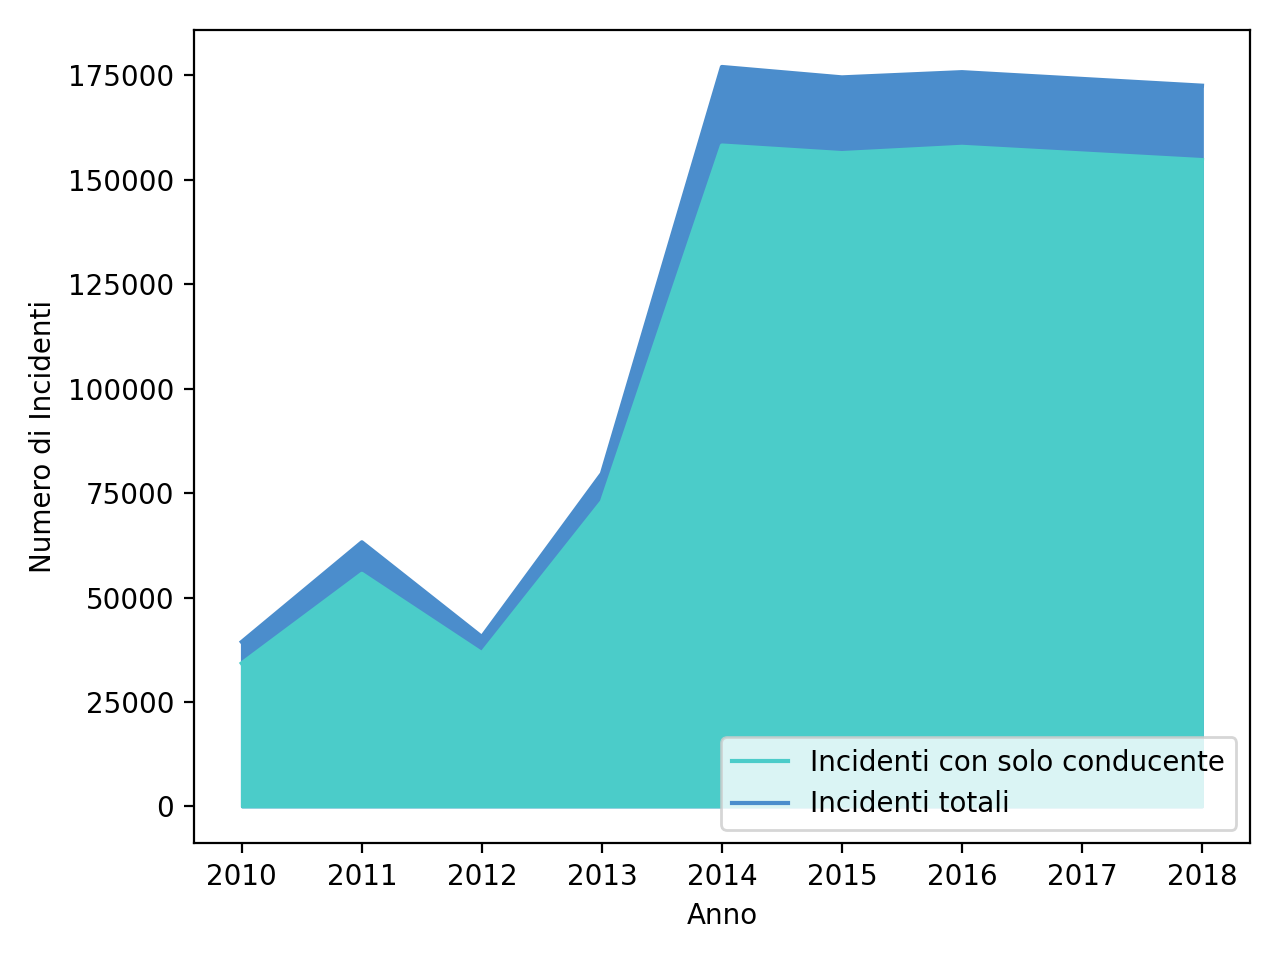
\includegraphics[width=\linewidth]{../src/incidenti/incidenti_senza_coords/anno/incremento_incidenti.png}
    \caption{Numero di incidenti all'anno, in cui è presente solo il conducente}
    \label{fig:incremento-incidenti}
\end{figure}

Nella figura \ref{fig:incremento-incidenti} è visibile l'aumento, tra 2013 e 2014, del 
numero di incidenti all'anno, il che supporterebbe l'ipotesi iniziale.
Tuttavia, il numero di sinistri nei quali è presente solo il conducente 
aumenta allo stesso modo, e gli incidenti con più di una persona nel veicolo 
salgono in maniera ancora maggiore. 
Queste tendenze sono visibili nella aumento dell'ampiezza dell'area blu, nel grafo 
\ref{fig:incremento-incidenti}.

L'ampio incremento di incidenti, a partire dal 2013, si arresta l'anno successivo, e dopo il 2015 
il numero di sinistri tende addirittura a diminuire, il che fa sospettare 
una modifica nella metodologia di raccolta dei dati, più che un cambiamento 
nel comportamento di molte persone. 

L'ipotesi del telefono cellulare come fattore di distrazione per il conducente, 
non è confermabile, perlomeno con i dati di cui si dispone. 
Va anche sottolineato che i dati utilizzati sono influenzati da svariati fattori, ed è 
possibile \quotestyle{ipotizzare} la prevalenza di uno di questi al di sopra degli altri, 
ma per confermare il collegamento sono necessarie indagini molto più approfondite di 
quelle eseguite. 

%\clearpage
\section{Dati Istat su orari e mesi}

%\clearpage
\subsection{Incremento dell'incidentalità in diversi orari}

Se si volesse stimare la distribuzione di traffico per orario, sicuramente una prima ipotesi 
deve essere quella di una curva più alta durante il giorno, con punto di minimo durante la notte. 
Il risultato atteso, inoltre, è quello di osservare due picchi più o meno marcati 
in corrispondenza delle fasce orarie di entrata e di uscita dal lavoro.
Una domanda che sorge spontanea, visto che i dati a disposizione si riferiscono agli incidenti, 
è se questi seguano lo stesso comportamento del traffico.

\begin{figure}
    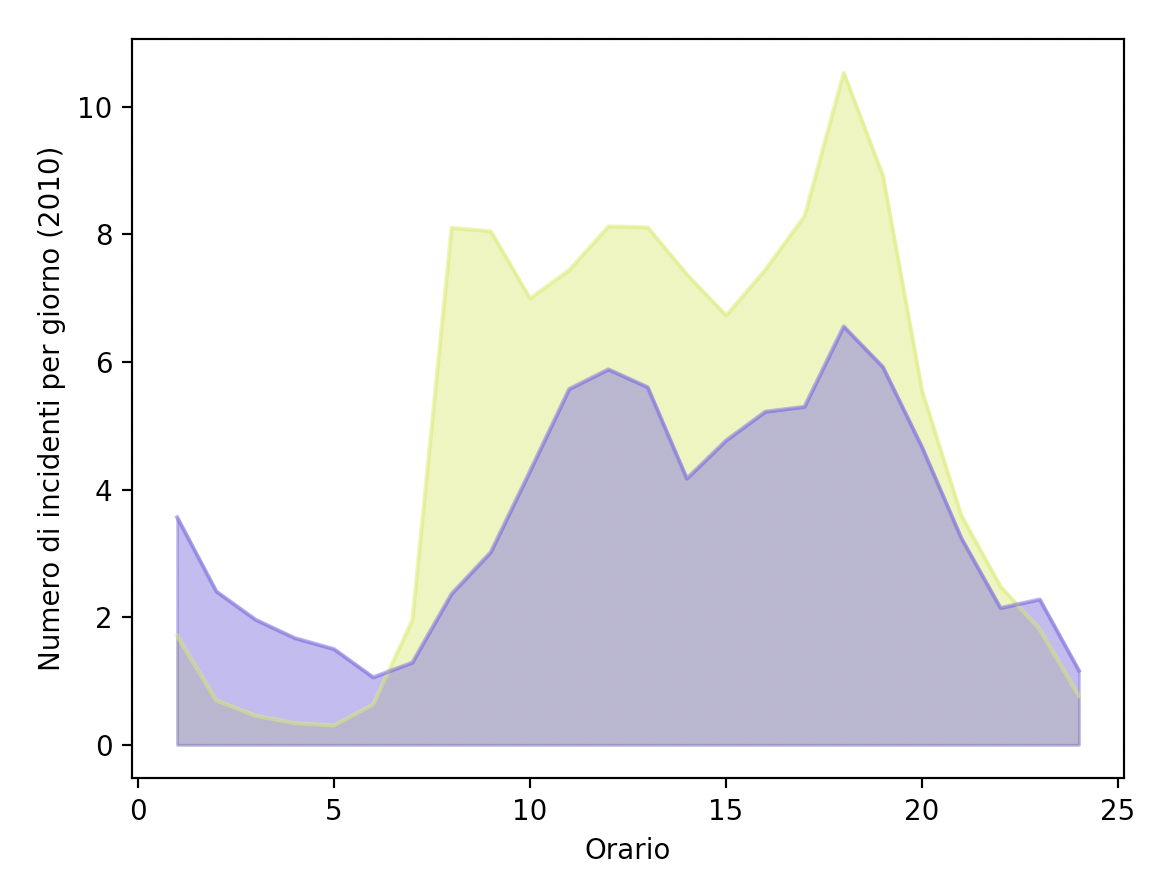
\includegraphics[width=\linewidth]{../src/incidenti/incidenti_senza_coords/ore_punta/week_weekend.png}
    \caption{Incidenti per ora}
    \label{fig:week-weekend}
\end{figure}

Tramite un semplice conteggio degli incidenti durante il weekend e, 
confrontandolo con il numero di quelli avvenuti durante la 
settimana lavorativa, si osserva come nel weekend avvengono più sinistri 
durante la sera e la notte, mentre in giornata durante la settimana.

Per quanto riguarda, le fasce orarie \quotestyle{di punta} definite precedentemente, 
sono stati presi in considerazione, per la mattina, gli orari dalle 7:00 alle 10:00, 
e per il pomeriggio, dalle 17:00 alle 19:00.

L'incremento durante la fascia oraria pomeridiana è subito osservabile nella figura 
\ref{fig:week-weekend}, dove si ha un incremento del $95.2$\% di incidenti rispetto 
alla media durante la settimana lavorativa. 
Durante il weekend, si osserva comunque un incremento, ma solamente del $61.1$\%.

Per le fasce orarie della mattina, è comunque presente un incremento di sinistri, ma questo 
ammonta al $34.6$\% alle 8:00, e al $80.6$\% alle 9:00, e nel weekend si ha addirittura un 
decremento di incidenti in entrambi gli orari, rispettivamente del $47.6$\% e $17.9$\%.

I grafi presentati indicano gli incidenti all'anno, normalizzati per numero di 
giorni settimanali e feriali, quindi gli incidenti totali della settimana sono divisi 
per cinque giorni, mentre quelli del weekend per due, come mostrato nel codice sottostante.

\begin{code}[language=Python]
ora_weekend = data[data['giorno'] > 5]['Ora'].value_counts().sort_index()
ora_week = data[data['giorno'] < 6]['Ora'].value_counts().sort_index()

ora_week /= 5 * 52
ora_weekend /= 2 * 52
\end{code}

Le informazioni ricavate ricalcano in modo particolarmente preciso, soprattutto nelle ore del 
pomeriggio, le ipotesi iniziali.

%\clearpage
\subsection{Incremento dell'incidentalità nelle fasce orarie della mattina}

I risultati della sezione precedente sembrano indicare che la maggior parte degli 
incidenti si verifica attorno alle 9:00 di mattina. 
Questa tendenza è vera anche nel caso in cui si isoli una città come Milano, 
che è la destinazione di molti pendolari della regione, probabilmente 
già in viaggio prima delle 9:00?

Selezionano solo gli incidenti nella provincia di Milano, mostrati nel grafo 
\ref{fig:week-weekend-milano}, è possibile individuare in modo più preciso
il primo picco di incidenti, quello durante le ore di punta mattutine.
In particolare si ha un incremento del $34.3$\% alle 8:00 rispetto alla media, 
che aumenta fino al $118.7$\% delle 9:00, nelle giornate lavorative.
D'altro canto, durante il weekend, il numero di incidenti alle 8:00 cala del $58.5$\% rispetto 
alla media e allo stesso modo alle 9:00, del $37$\%.

\begin{figure}
    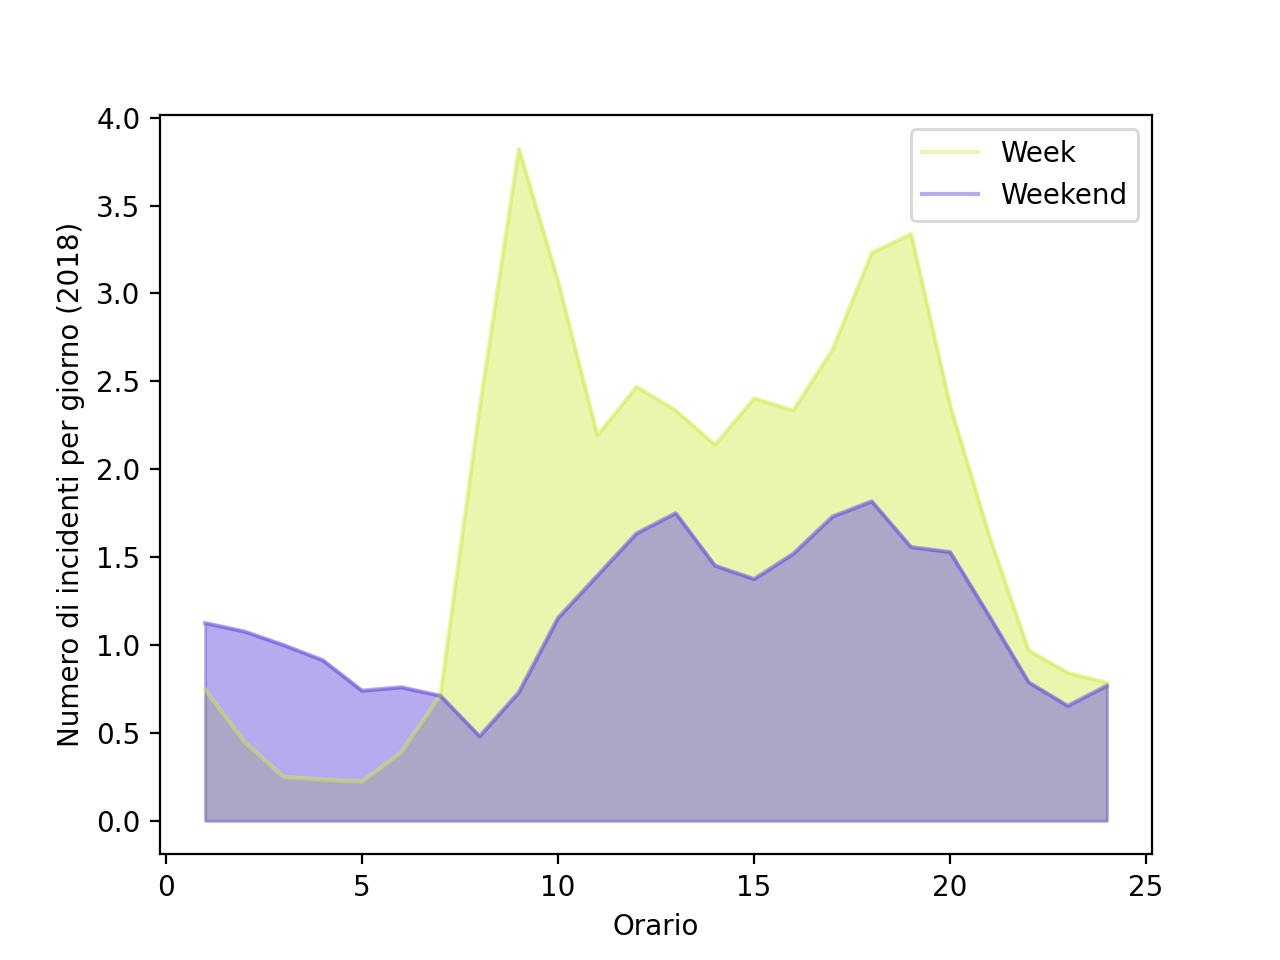
\includegraphics[width=\linewidth]{../src/incidenti/incidenti_senza_coords/ore_punta/week_weekend_milano.png}
    \caption{Incidenti per ora a Milano}
    \label{fig:week-weekend-milano}
\end{figure}

A Milano, dunque, si ha un incremento percentuale di incidenti ancora maggiore 
rispetto al resto di Italia, e il flusso di pendolari, alla guida in orari precedenti 
alle 9:00 di mattina, non sembra influenzare il volume di sinistri.

\subsection{Correlazione tra incidenti e traffico}

Fino a questo momento, si è parlato di incidenti senza alcun tipo di contesto, in 
particolare senza tenere conto del numero di automobili presenti sulle strade. 
\'E chiaro che uno dei principali fattori che causa incidenti sia proprio 
il numero di automobili presenti, sarebbe interessante riuscire a isolare 
l'impatto dell traffico, nelle diverse ore della giornata.

Un primo problema da affrontare è quello di individuare informazioni sul 
numero di macchine presenti su strada in diverse fasce orarie. 
Per quanto un dataset contenente questi dati non sia stato trovato, 
è possibile realizzare una stima di questo carattere a Milano, 
a partire dal 2011, fino al 2016, utilizzando i dataset sul numero 
degli accessi all'area C.

\begin{figure}
    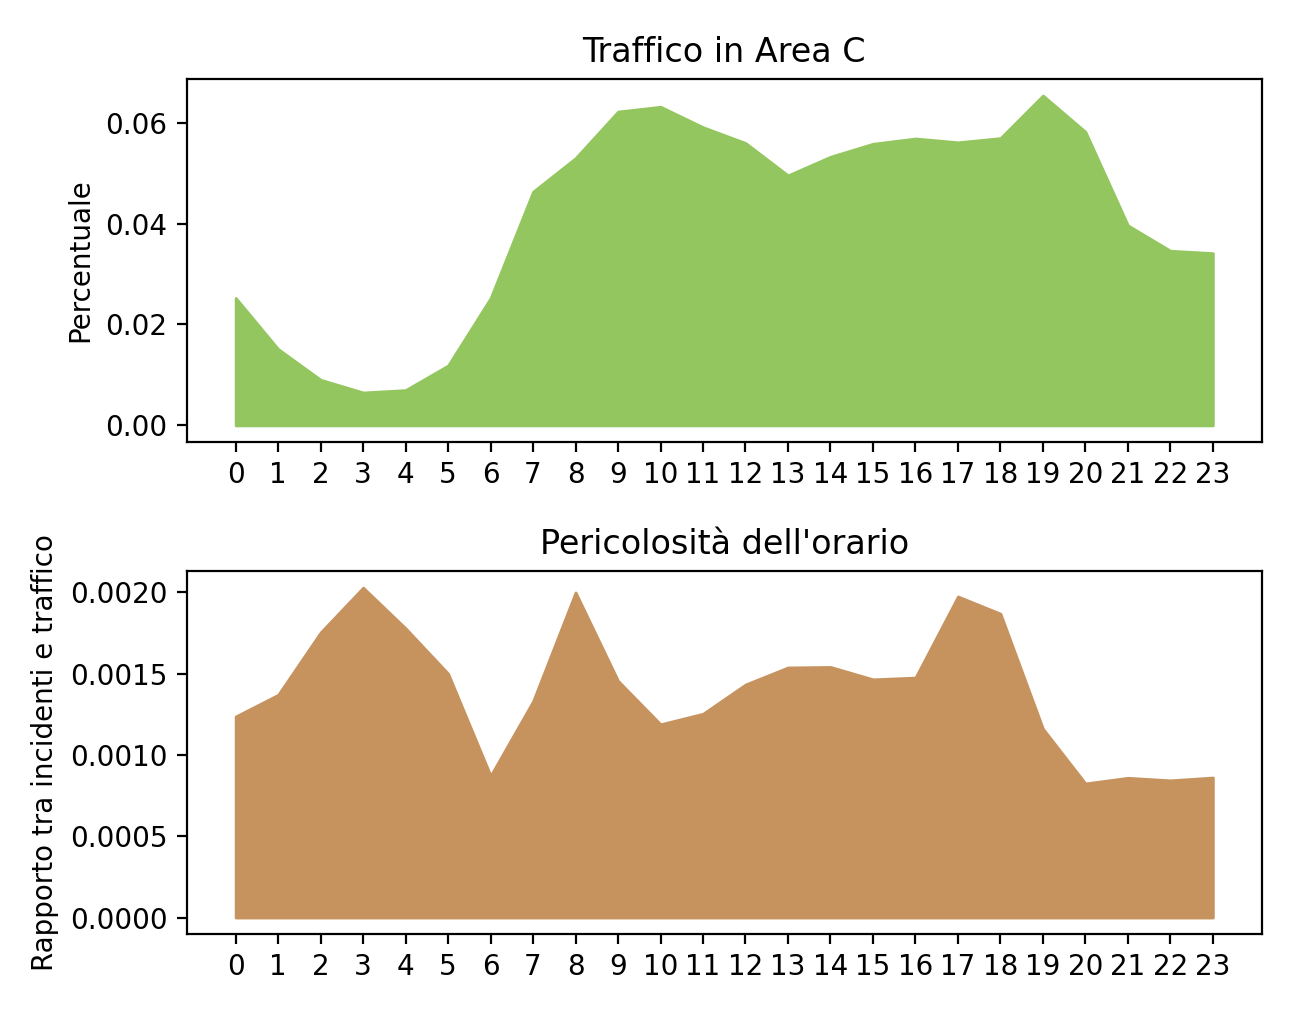
\includegraphics[width=\linewidth]{../src/area_c/rapporto_orario.png}
    \caption{Rapporto tra incidenti e traffico per orario a Milano}
    \label{fig:rapporto-incidenti-traffico}
\end{figure}

L'immagine \ref{fig:rapporto-incidenti-traffico} contiene, sulla sinistra, 
la percentuale di accessi in area C a una determinata 
ora\footnote{Si sono utilizzati i dati dell'anno 2016, perchè non si sono trovati 
dataset più recenti per quanto riguarda gli accessi all'area C di Milano}, 
e nel grafo a destra, il numero di incidenti a Milano, pesati in base al 
questa stima del traffico.

Si osservano molte similitudini tra la stima realizzata tramite gli ingressi 
in area C, rappresentata nel grafo sinistro della 
figura \ref{fig:rapporto-incidenti-traffico} e l'immagine \ref{fig:week-weekend-milano}, 
raffigurante gli incidenti a Milano divisi per orario. 
In particolare, tra traffico in area C a Milano e 
numero incidenti per orario, si è calcolato un coefficiente di Pearson uguale a $0.877$, 
quindi è possibile dire che i due siano dataset linearmente correlati.

\begin{code}
# eseguito con dati del 2016
accessi_area_c_per_ora = pd.Series()
for f in data['hour'].unique():
    accessi_area_c_per_ora = accessi_area_c_per_ora.append(
        pd.Series(data[data['hour'] == f]['totale'].sum()), 
        ignore_index=True
        )

incidenti_per_ora = data[data['provincia'] == 15]['ora'].value_counts().sort_index()

correlazione = accessi_area_c_per_ora.corr(incidenti_per_ora)
\end{code}

Per quanto riguarda invece, il grafo nella metà bassa della 
figura \ref{fig:rapporto-incidenti-traffico}, sono presenti tre picchi di 
con orari particolarmente pericolosi, uno alle 3:00 di mattina, uno alle 
8:00 e l'ultimo alle 18:00. 

Di questi, il primo è possibile che sia dovuto allo scarso volume di accessi 
all'area C in questo orario, visto che alle 3:00 di notte si ha il minimo volume di 
traffico della giornata, mentre gli altri due sono certamente dovuti all'alto 
numero di incidenti, in quanto il traffico in questi orari è pienamente nella media.
Gli ultimi due orari, inoltre, sono i due orari di punta coincidenti con l'inizio 
e la fine della giornata lavorativa per la maggior parte delle persone. 
Chiaramente, con l'aumento del numero di persone in viaggio, aumenta anche il 
numero di \quotestyle{pericoli} a cui ogni conducente deve prestare attenzione.

\subsection{Incidentalità in orari notturni}

Nel grafo \ref{fig:week-weekend}, si è potuto osservare come, durante le 
ore notturne, il comportamento degli incidenti tra settimana lavorativa e weekend 
sia l'opposto, con maggior numero di sinistri durante le ore notturne del 
Sabato e della Domenica.
Nella figura \ref{fig:ore-notte} sono raffigurate le principali ore della notte, divise tra 
settimana lavorativa e weekend.

Chiaramente, durante il weekend si hanno un numero più alto di incidenti negli orari serali e 
notturni, in particolare si hanno in media $5$ incidenti per serata in settimana, mentre il numero 
quasi raddoppia a $9.4$ durante il Sabato e la Domenica sera.

\begin{code}
notte = data[(data['Ora'] < 7) | (data['Ora'] > 22)]
ora_notte_week = notte[notte['giorno'] < 6]['Ora'].value_counts().sort_index()
ora_notte_weekend = notte[notte['giorno'] > 5]['Ora'].value_counts().sort_index()

ora_notte_week /= 5 * 52  
ora_notte_weekend /= 2 * 52
\end{code}

Il traffico, stimato tramite gli accessi all'area C, conferma questa tendenza?
\begin{figure}
    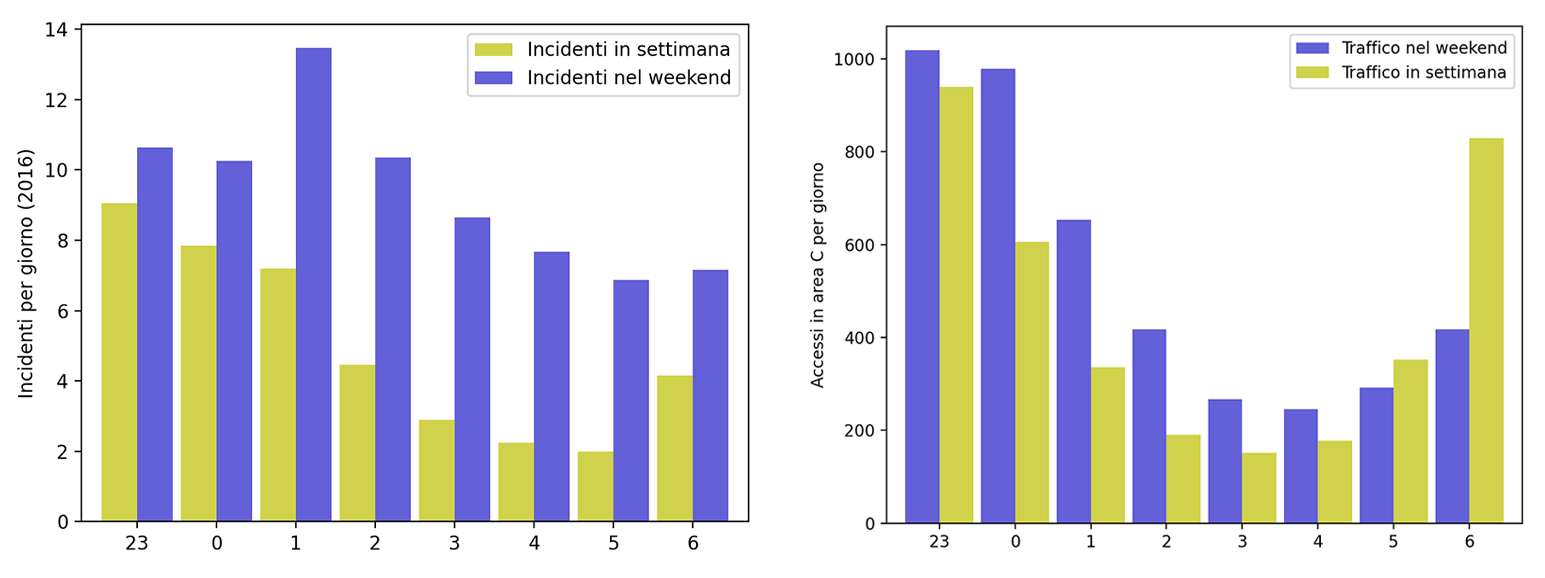
\includegraphics[width=\linewidth]{img_unite/ore_punta.png}
    \caption{Incidenti e traffico durante ore serali o notturne}
    \label{fig:ore-notte}
\end{figure}

Premettendo che la differenza di traffico tra settimana lavorativa e 
weekend in orari serali non è molta, il divario maggiore è presente alle ore 6:00 
in favore del traffico in settimana, mentre il traffico nel weekend è maggiore in 
quasi tutte le altre ore.

Una volta ottenuti questi risultati, è possibile ricavare quali siano le ore 
più pericolose, calcolando il rapporto tra incidenti e traffico per orario.
Il risultato di questo procedimento è rafficurato nel grafo \ref{fig:rapp-inc-traff}.

\begin{figure}
    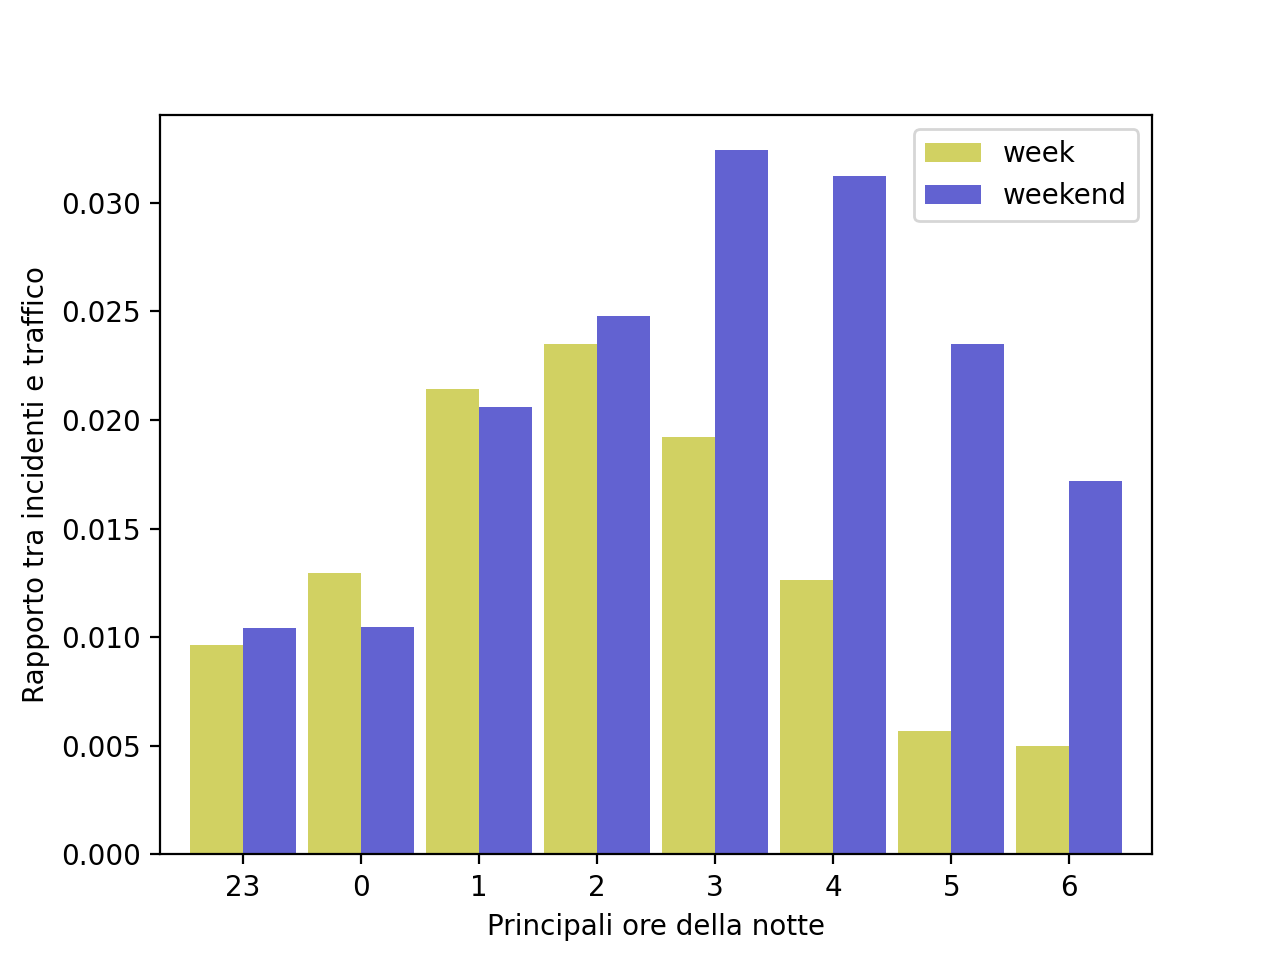
\includegraphics[width=\linewidth]{../src/area_c/rapporto_inc_notte.png}
    \caption{Rapporto tra incidenti e traffico durante ore serali o notturne}
    \label{fig:rapp-inc-traff}
\end{figure}

Durante il weekend, le ore più pericolose sono tra le 3:00 e le 4:00 di notte. 
D'altra parte, per la settimana lavorativa, gli orari più pericolosi sono quelli 
tra l'una e le tre di notte, con un numero di incidenti rapportato al 
traffico molto minore. 

I risultati sembrano essere in linea con l'idea che, nel weekend, il maggior 
numero di incidenti avvenga in ore più tarde a causa della movida, mentre durante 
la settimana lavorativa meno persone siano sveglie nelle ore notturne.

%\clearpage
\subsection{Quanto influiscono le vacanze estive sull'incidentalità?}

Sarebbe interessante individuare eventuali cali o incrementi di incidenti 
su intervallo mensile.
Il dataset sugli accessi all'area C è presente, nel caso della divisione per 
mese, fino all'anno 2018, tuttavia il campo \columnstyle{mese} è presente nei 
dati Istat solo fino all'anno 2013, ed è sostituito successivamente 
dalla colonna \columnstyle{trimestre}, dunque i grafi sull'argomento prenderanno 
in considerazione quest'annata più recente.

\begin{figure}
    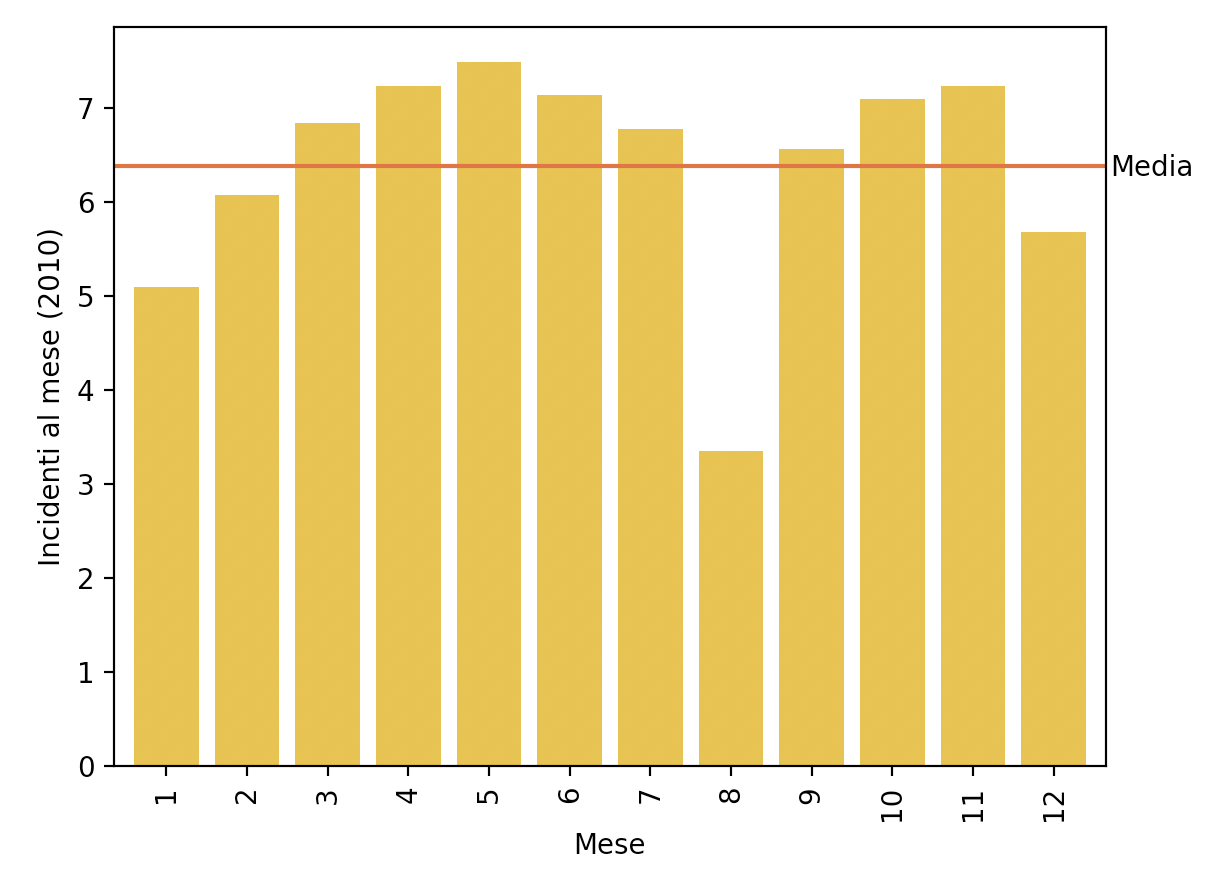
\includegraphics[width=\linewidth]{../src/incidenti/incidenti_senza_coords/mese_incidenti/milano_mese.png}
    \caption{Incidenti per mese in Milano nel 2013}
    \label{fig:milano-mese}
\end{figure}

Nel grafo \ref{fig:milano-mese} si nota un chiaro calo di incidenti nel mese di 
Agosto in provincia di Milano. 
La percentuale di decremento è riportata nella tabella sottostante, assieme agli 
altri anni per cui sono disponibili i dati.

\begin{center}
    \def\arraystretch{1.5}%  
    \begin{tabular}{ |c|c| } 
        \hline
        Anno & Decremento in Agosto \\ 
        \hline
        2010 & 47.4\%  \\ 
        \rowcolor{TableGray}
        2011 & 35.14\% \\
        2012 & 45.46\% \\
        \rowcolor{TableGray}
        2013 & 41.37 \% \\
        \hline
    \end{tabular}
\end{center}

Per quanto possano esserci molti fattori che contribuiscono a questa tendenza di 
decremento di sinistri, uno di quelli più influenti deve essere la partenza 
di persone per le vacanze estive.

Un modo per testare questa teoria è controllare se il traffico, 
stimato tramite i dati sugli accessi in area C, cala durante il mese di 
Agosto a Milano. 
A supporto dell'ipotesi iniziale, nella figura \ref{fig:stima-traffico-mensile}, 
è visibile un calo di accessi all'area C durante i mesi di Giugno, Luglio e Agosto.

\begin{figure}
    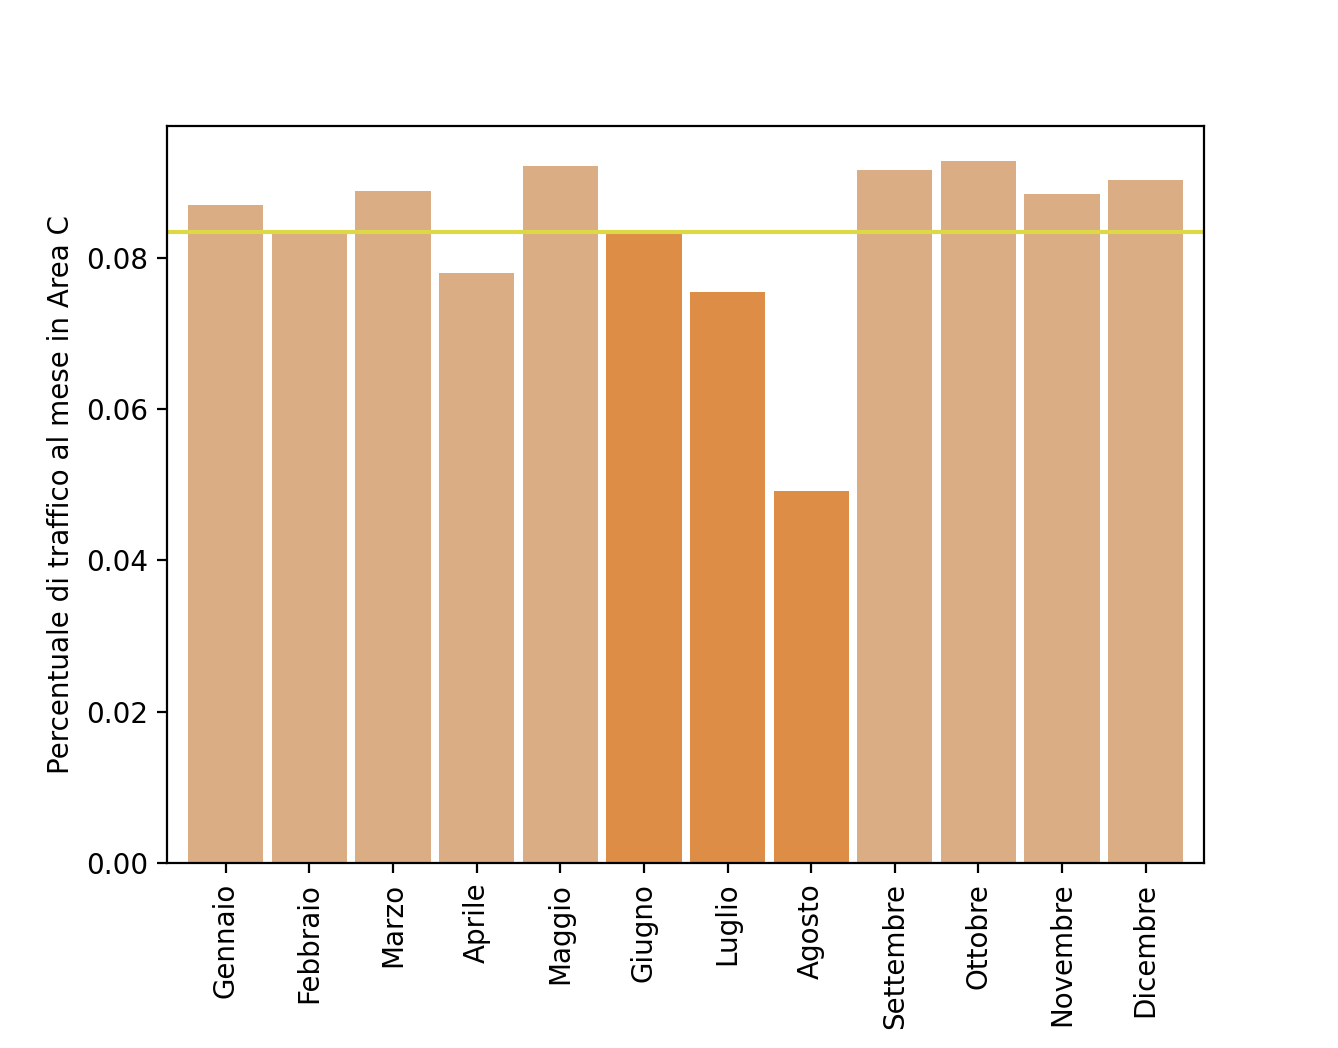
\includegraphics[width=\linewidth]{../src/area_c/stima_traffico_mese.png}
    \caption{Stima del traffico a Milano per mese, tramite accessi all'area C}
    \label{fig:stima-traffico-mensile}
\end{figure}

Una volta ottenuta una stima del traffico, è possibile calcolare quali mesi 
siano più pericolosi dal punto di vista degli incidenti, rapportando il numero di 
sinistri al numero di accessi in area C mensile.

\begin{figure}
    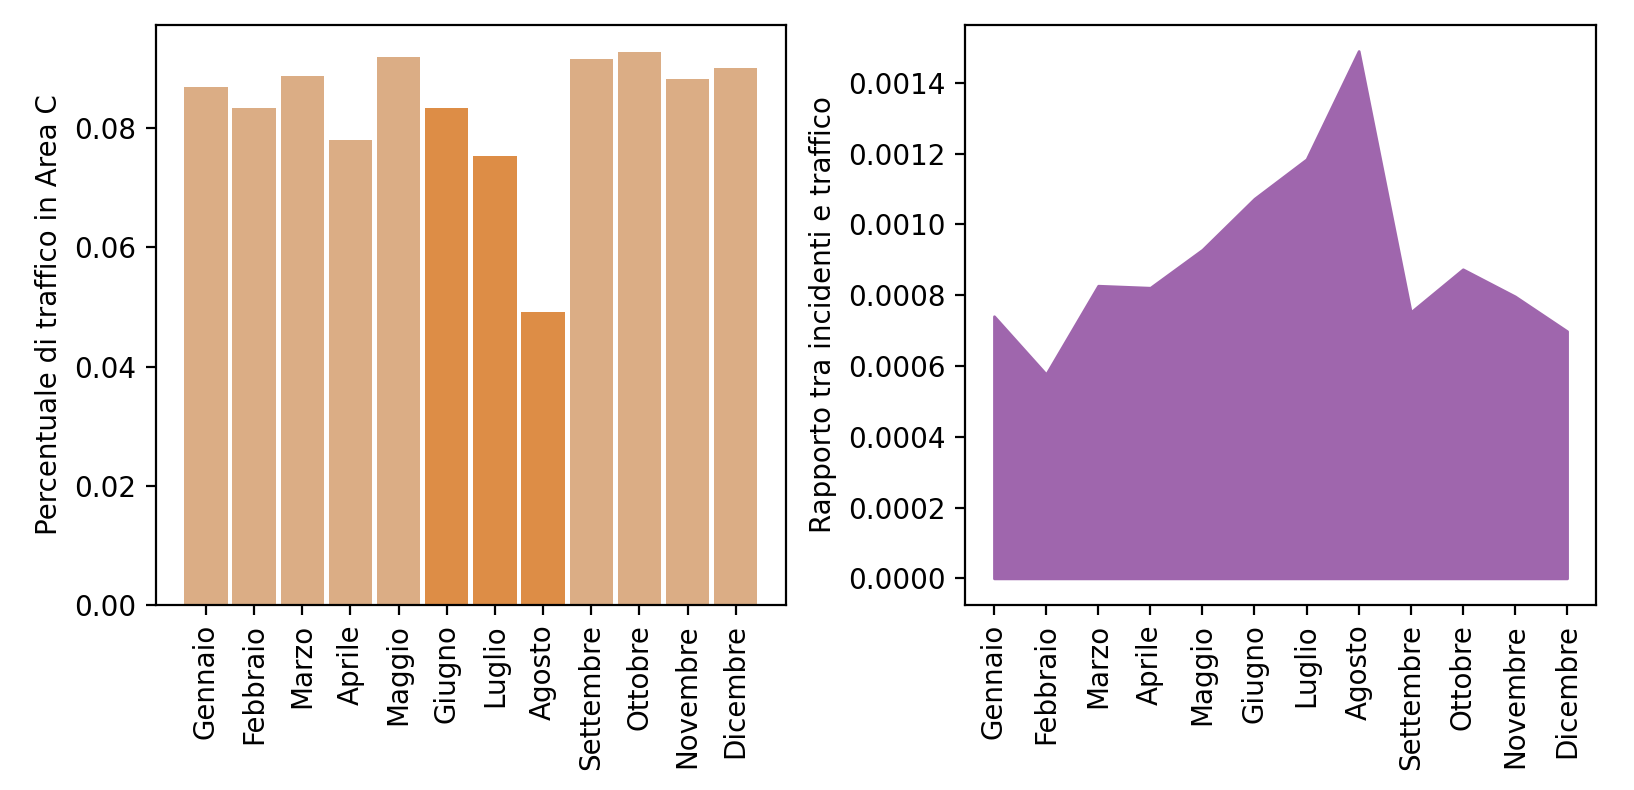
\includegraphics[width=\linewidth]{../src/area_c/rapporto_mese.png}
    \caption{Incidenti al mese, tenendo conto del traffico nello stesso periodo (2012)}
    \label{fig:incidenti-traffico-mese}
\end{figure}

L'immagine \ref{fig:incidenti-traffico-mese} contiene due grafi, 
il primo riguardante la frazione di traffico annuale che interessa ogni mese, 
mentre il secondo raffigura il rapporto tra il numero di incidenti mensili, e il traffico 
stimato\footnote{Si è utilizzato l'anno 2012 perchè è il primo anno contenente tutti i dati completi, 
tutti gli altri anni hanno mesi o campi mancanti, per esempio il file corrispondente all'anno 
2013 non ha le misurazioni per tutto il mese di Dicembre}.
Nel secondo grafo della figura \ref{fig:incidenti-traffico-mese}, si osserva come, 
nonostante Agosto abbia il minor numero di incidenti mensili, 
una volta tenuto conto della minore quantità di traffico, risulti essere 
il mese più pericoloso.

A partire dal 2014, il campo \columnstyle{mese} è stato convertito nella 
colonna \columnstyle{trimestre}.
La figura \ref{fig:milano-trimestri} mostra la quantità di incidenti per 
trimestre per ogni anno a partire dal 2010 fino al 2018.

\begin{figure}
    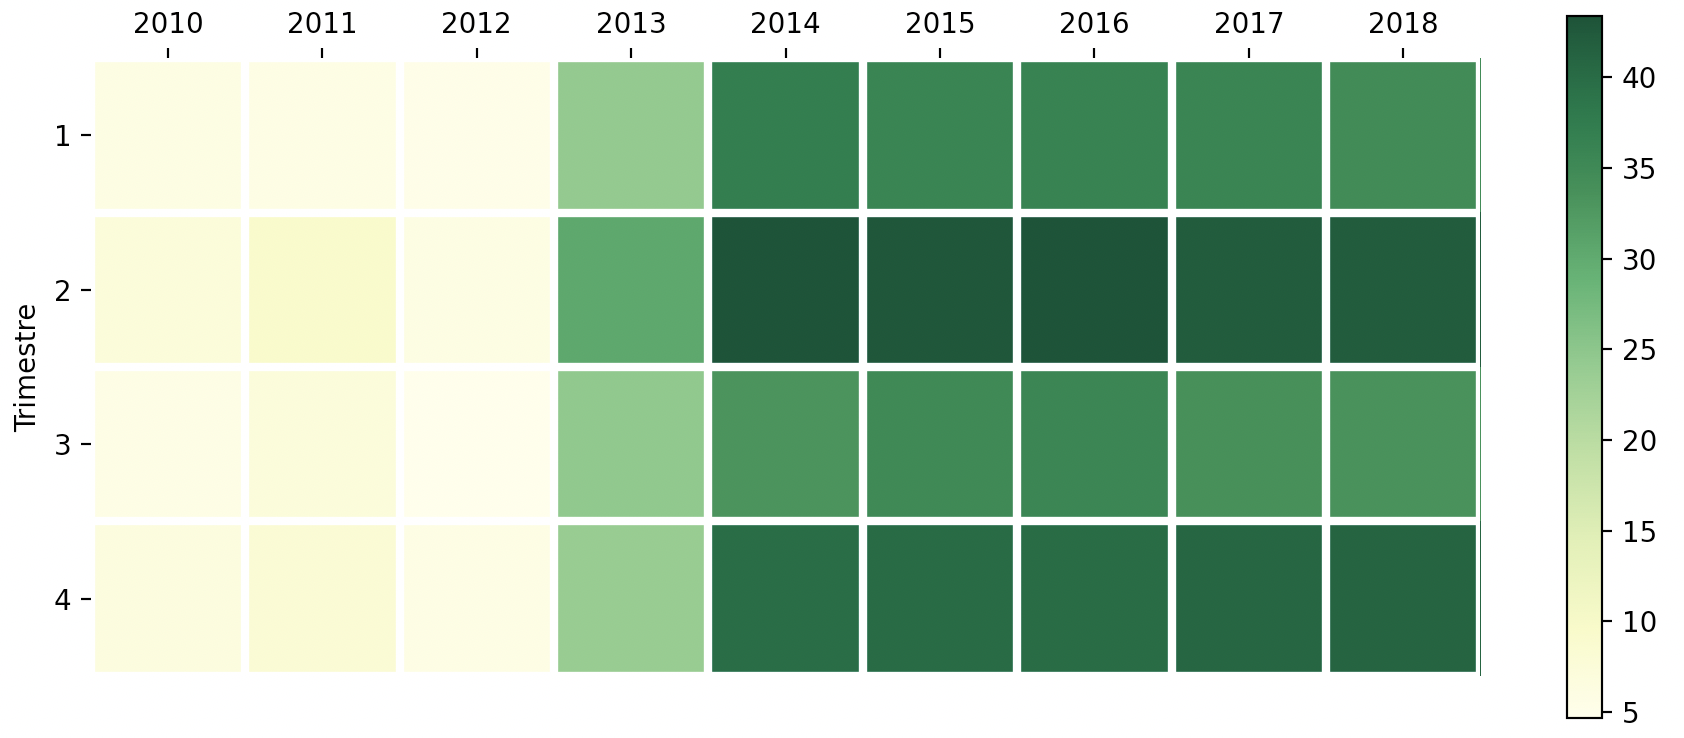
\includegraphics[width=\linewidth]{../src/incidenti/incidenti_senza_coords/mese_incidenti/trimestri.png}
    \caption{Incidenti per trimestre a Milano}
    \label{fig:milano-trimestri}
\end{figure}

\'E possibile osservare, anche in questo grafo, l'aumento di sinistri a partire dall'anno 2013, 
di cui si è parlato nel capitolo riguardante l'utilizzo del cellulare all guida.

Anche nel caso dei trimestri, quello estivo ha un numero minore di incidenti. 
Tuttavia, in questo caso, il volume del primo trimestre è comparabile con quello del terzo 
(estivo), mentre durante il secondo e il quarto avvengono decisamente più incidenti.


\subsection{In località di mare gli incidenti aumentano in estate?}

Visto il grafo in figura \ref{fig:milano-mese}, una domanda che sorge spontanea, è se 
il numero basso di incidenti in Agosto corrisponda con un numero alto di sinistri in 
altre località di vacanza. 
In altre parole, visto che un gran numero di persone si spostano in macchina 
in altre regioni durante il mese di Agosto, questa differenza di traffico è osservabile 
nel numero di incidenti?

\begin{figure}
    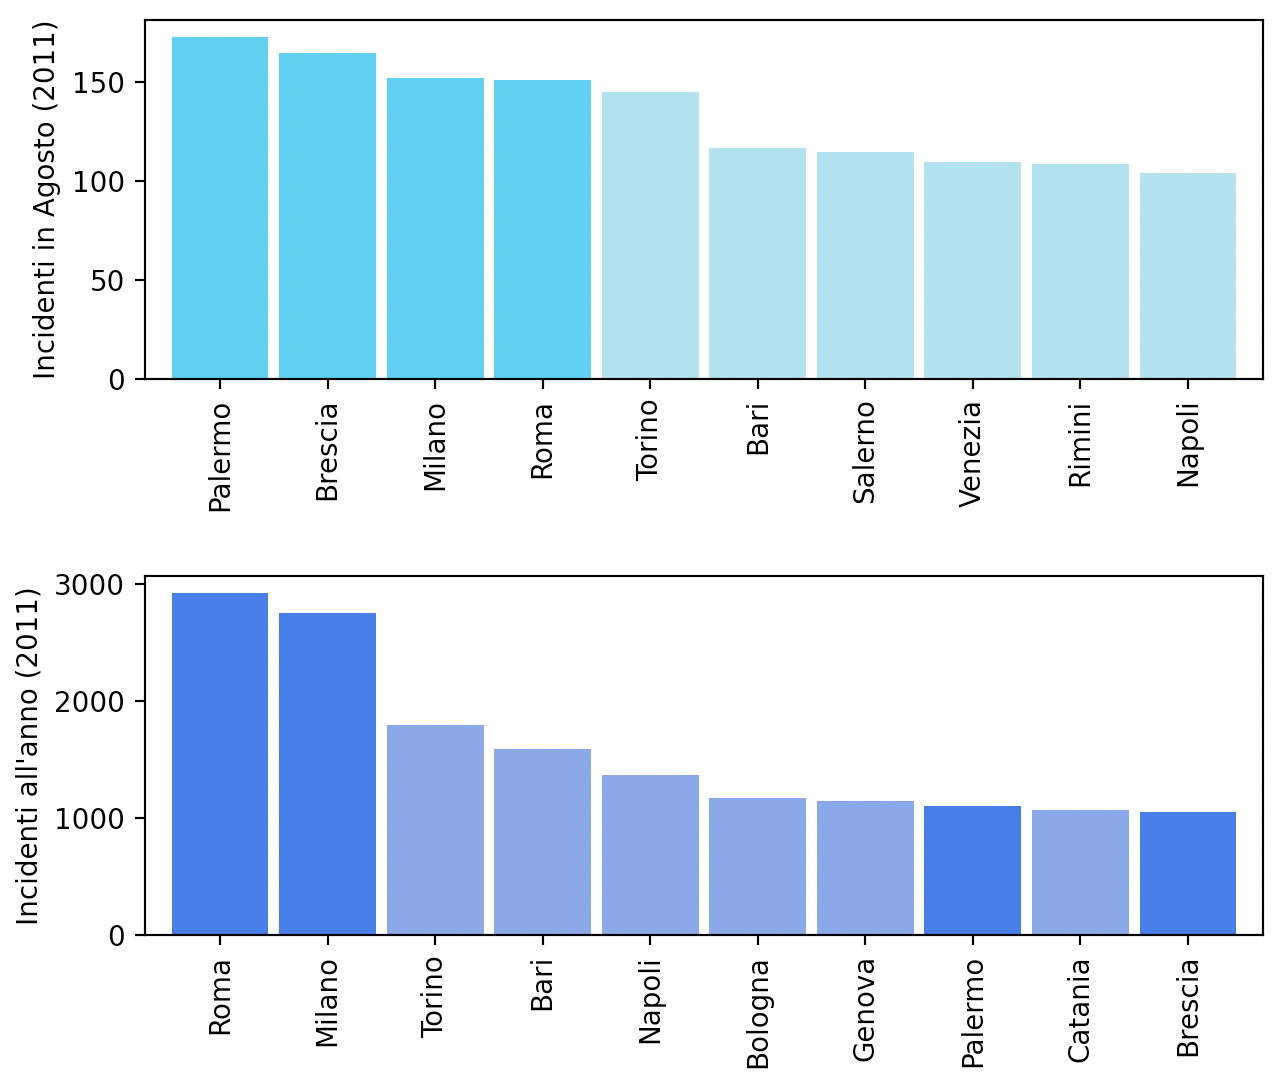
\includegraphics[width=\linewidth]{../src/incidenti/incidenti_senza_coords/mese_incidenti/mesi_estivi.png}
    \caption{Prime 10 province per incidenti in Agosto rispetto a tutto l'anno}
    \label{fig:mesi-estivi}
\end{figure}

Nalla figura \ref{fig:mesi-estivi} sono elencate le province con maggiore incidentalità 
in Agosto rispetto a tutto l'anno. In particolare, ad aumentare in volume sono le 
province di Brescia e Palermo.

Il comportamento rappresentato nel grafico, tuttavia, è unico dell'anno 2011, in quanto, 
per gli altri due anni di cui si dispone dei dati (2012 e 2013), 
Milano e Roma hanno il primato di incidenti sia per l'anno, come ci si attende, che per il 
mese di Agosto individuale, nel 2011 occupato da Palermo.

D'altra parte, se si pensasse di comparare più nel dettaglio alcune province, 
meta di vacanze estive con Milano, ciò che ci si aspetterebbe da queste ultime sarebbe 
di avere un incremento di incidenti nei mesi di Luglio e 
Agosto\footnote{Si è utilizzato l'anno più recente per i dati a disposizione, 
a partire dal 2014 non sono più disponibili dati riguardanti il mese}.
Per eseguire questo confronto sono state prese in considerazione le località di Rimine e Palermo, 
per mostrare che alcune province, come la prima, confermano l'ipotesi, mentre altre, 
come la seconda, possono essere usate come controesempio.

\begin{figure}
    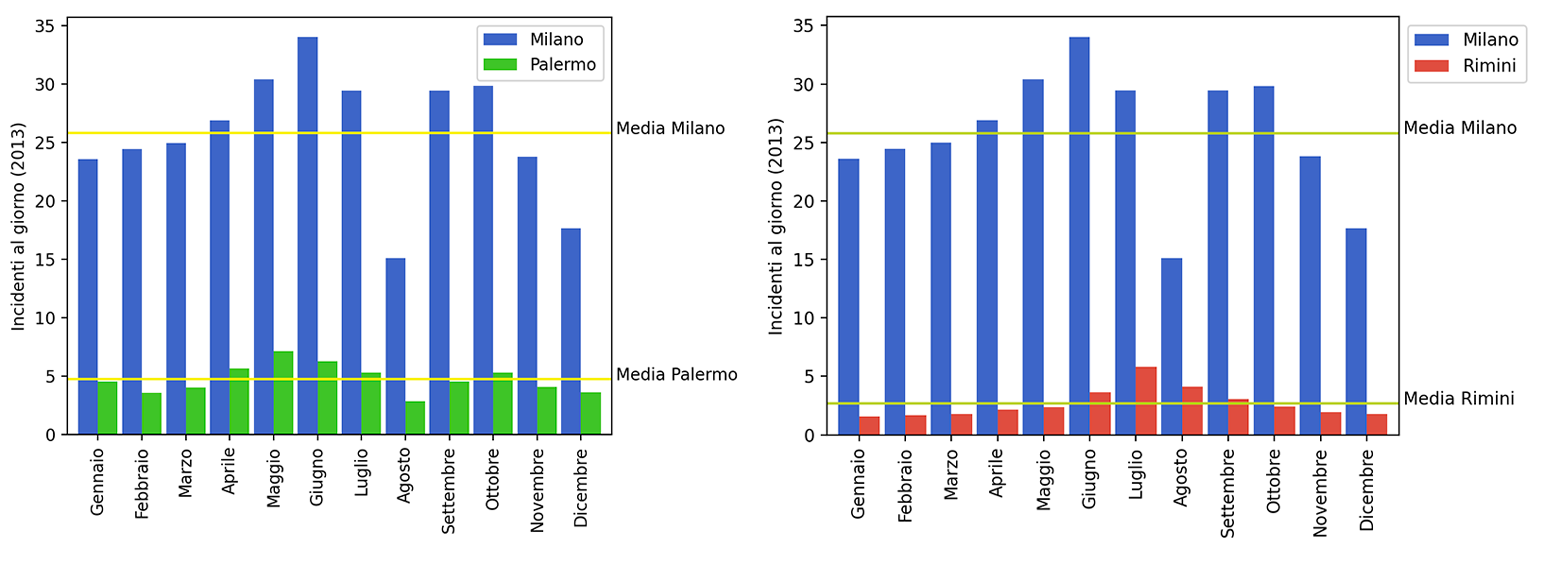
\includegraphics[width=\linewidth]{img_unite/milano_rimini_palermo.png}
    \caption{Incidenti per mese a Milano, Rimini e Palermo}
    \label{fig:milano-rimini}
\end{figure}

Il confronto tra Milano e Rimini è raffigurato nell'immagine sinistra della 
figura \ref{fig:milano-rimini}e, nonostante a Milano avvengano un numero molto maggiore di 
incidenti rispetto alla provincia Emiliana, nei mesi estivi, 
il numero di sinistri a Rimini è superiore alla media annuale, 
mentre per Milano è inferiore. 
Inoltre, a Milano si ha una tendenza di diminuzione di incidenti in Agosto e nei 
mesi invernali, mentre a Rimini si ha incremento nei mesi estivi.

Nella provincia di Palermo, visibile nel grafo destro in figura \ref{fig:milano-rimini}, 
d'altra parte, non risulta che nessun mese abbia un numero di incidenti 
particolarmente più alto della media, anzi la tendenza sembra imitare il comportamento di 
Milano, con Agosto e i mesi invernali più bassi della media.

Nella seguente tabella, sono indicate le percentuali di aumento per anno del numero di 
incidenti a Rimini.
L'incremento più o meno constante in ogni anno, conferma questo fenomeno come un trend 
annuale, e non un outlier dovuto a un 2011 fuori dalla norma.

\begin{center}
    \def\arraystretch{1.5}%  
    \begin{tabular}{ |c|c|c| } 
    \hline
    Anno & Luglio   & Agosto \\ 
    \hline
    \rowcolor{TableGray}
    2010 & 101.72\% & 63.75 \% \\ 
    2011 & 54.6  \%  & 60.49\% \\
    \rowcolor{TableGray}
    2012 & 75.97 \%  & 45.93\%\\
    2013 & 116.37\% & 51.82 \%\\
    \hline
    \end{tabular}
\end{center}

Una domanda che sorge spontanea, è se i calcoli realizzati valgano anche nelle regioni 
del nord Italia, e se questi permettano di individuare un incrementi di incidenti in 
inverno, a segnalare la stagione sciistica.
Nel grafo raffigurante gli incidenti per mese della Valle d'Aosta, 
in figura \ref{fig:aosta}, si notano incrementi dell'incidentalità 
nei mesi di Giugno e Settembre, tuttavia, nei mesi invernali, il numero di sinistri è 
generalmente più basso rispetto alla media.

\begin{figure}
    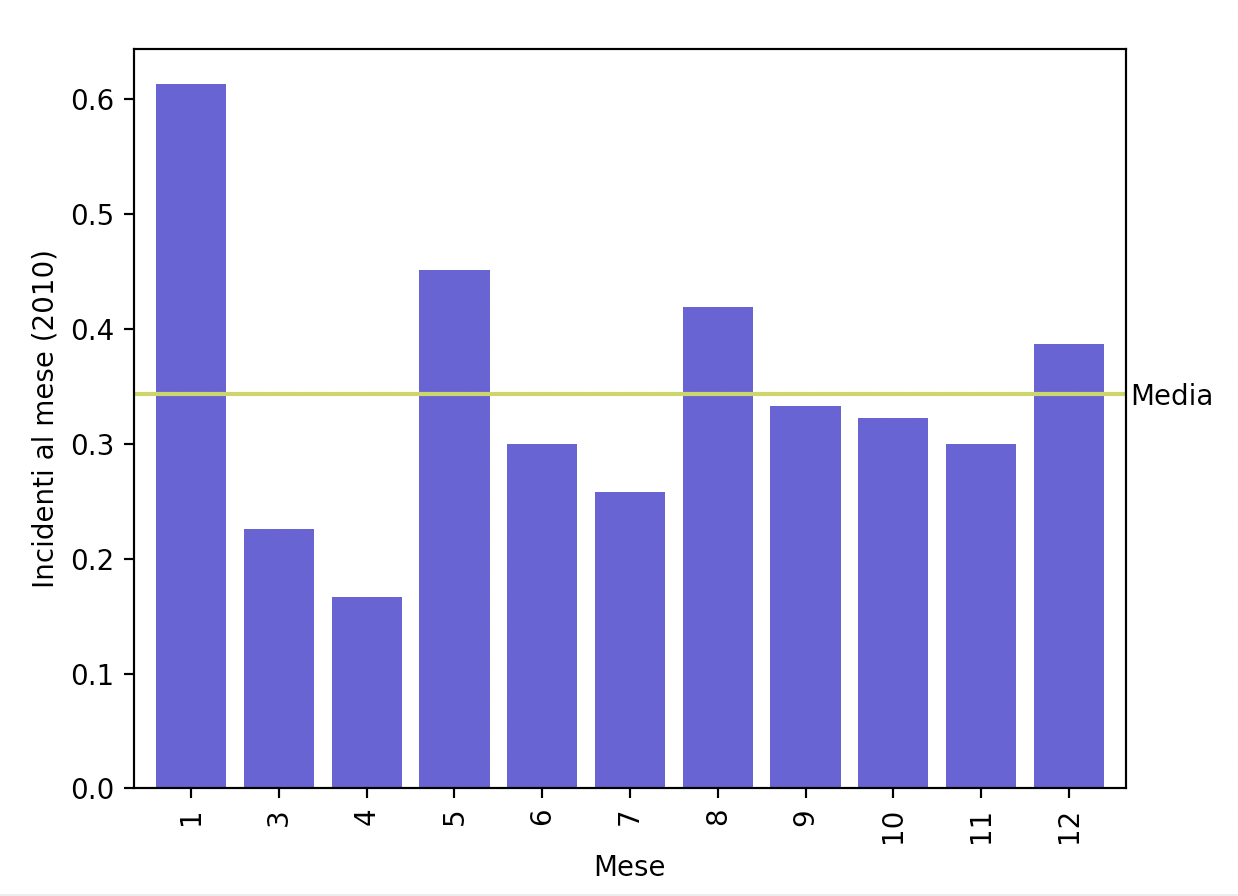
\includegraphics[width=\linewidth]{../src/incidenti/incidenti_senza_coords/mese_incidenti/aosta_mese.png}
    \caption{Incidenti per mese Valle d'Aosta}
    \label{fig:aosta}
\end{figure}

La prima cosa che è possibile controllare, è se questa tendenza avvenga ogni anno. 
Nella tabella sottostante sono stati riportati gli incrementi percentuali di incidenti 
rispetto alla media annuale, per ogni anno disponibile.

\begin{center}
    \def\arraystretch{1.5}%  
    \begin{tabular}{ |c|c|c| } 
    \hline
    Anno & Gennaio & Agosto \\ 
    \hline
    \rowcolor{TableGray}
    2010 & 78.48\%  & -2.93 \%\\ 
    2011 & -32.12\% & 124.0 \%\\
    \rowcolor{TableGray}
    2012 & -41.44\% & 52.25 \% \\
    2013 & -24.63\% & -15.21\% \\
    \hline
    \end{tabular}
\end{center}

Il comportamento degli incidenti in Valle d'Aosta mostrato, oltre che in tabella, 
anche in figura \ref{fig:aosta-rimini-milano-trimestre} è molto inconsistente, 
soprattutto in Agosto.
Va specificato che la taglia del campione con cui si sta lavorando, per questa provincia, 
è molto piccolo, e sicuramente influisce sulle percentuali di incremento e decremento 
degli incidenti.
Nonostane ciò, assumendo che Gennaio 2010 sia un outlier, il numero di incidenti in 
questo mese è sempre in decremento rispetto alla media, con percentuali abbastanza alte.

Per avere una visione di insieme delle tendenze annuali, è possibile tracciare 
il grafo \ref{fig:aosta-rimini-milano-trimestre}, contenente gli incidenti divisi 
per trimestre dove, per esempio, per primo trimestre si 
intende Gennaio, Febbraio e Marzo.

\begin{figure}
    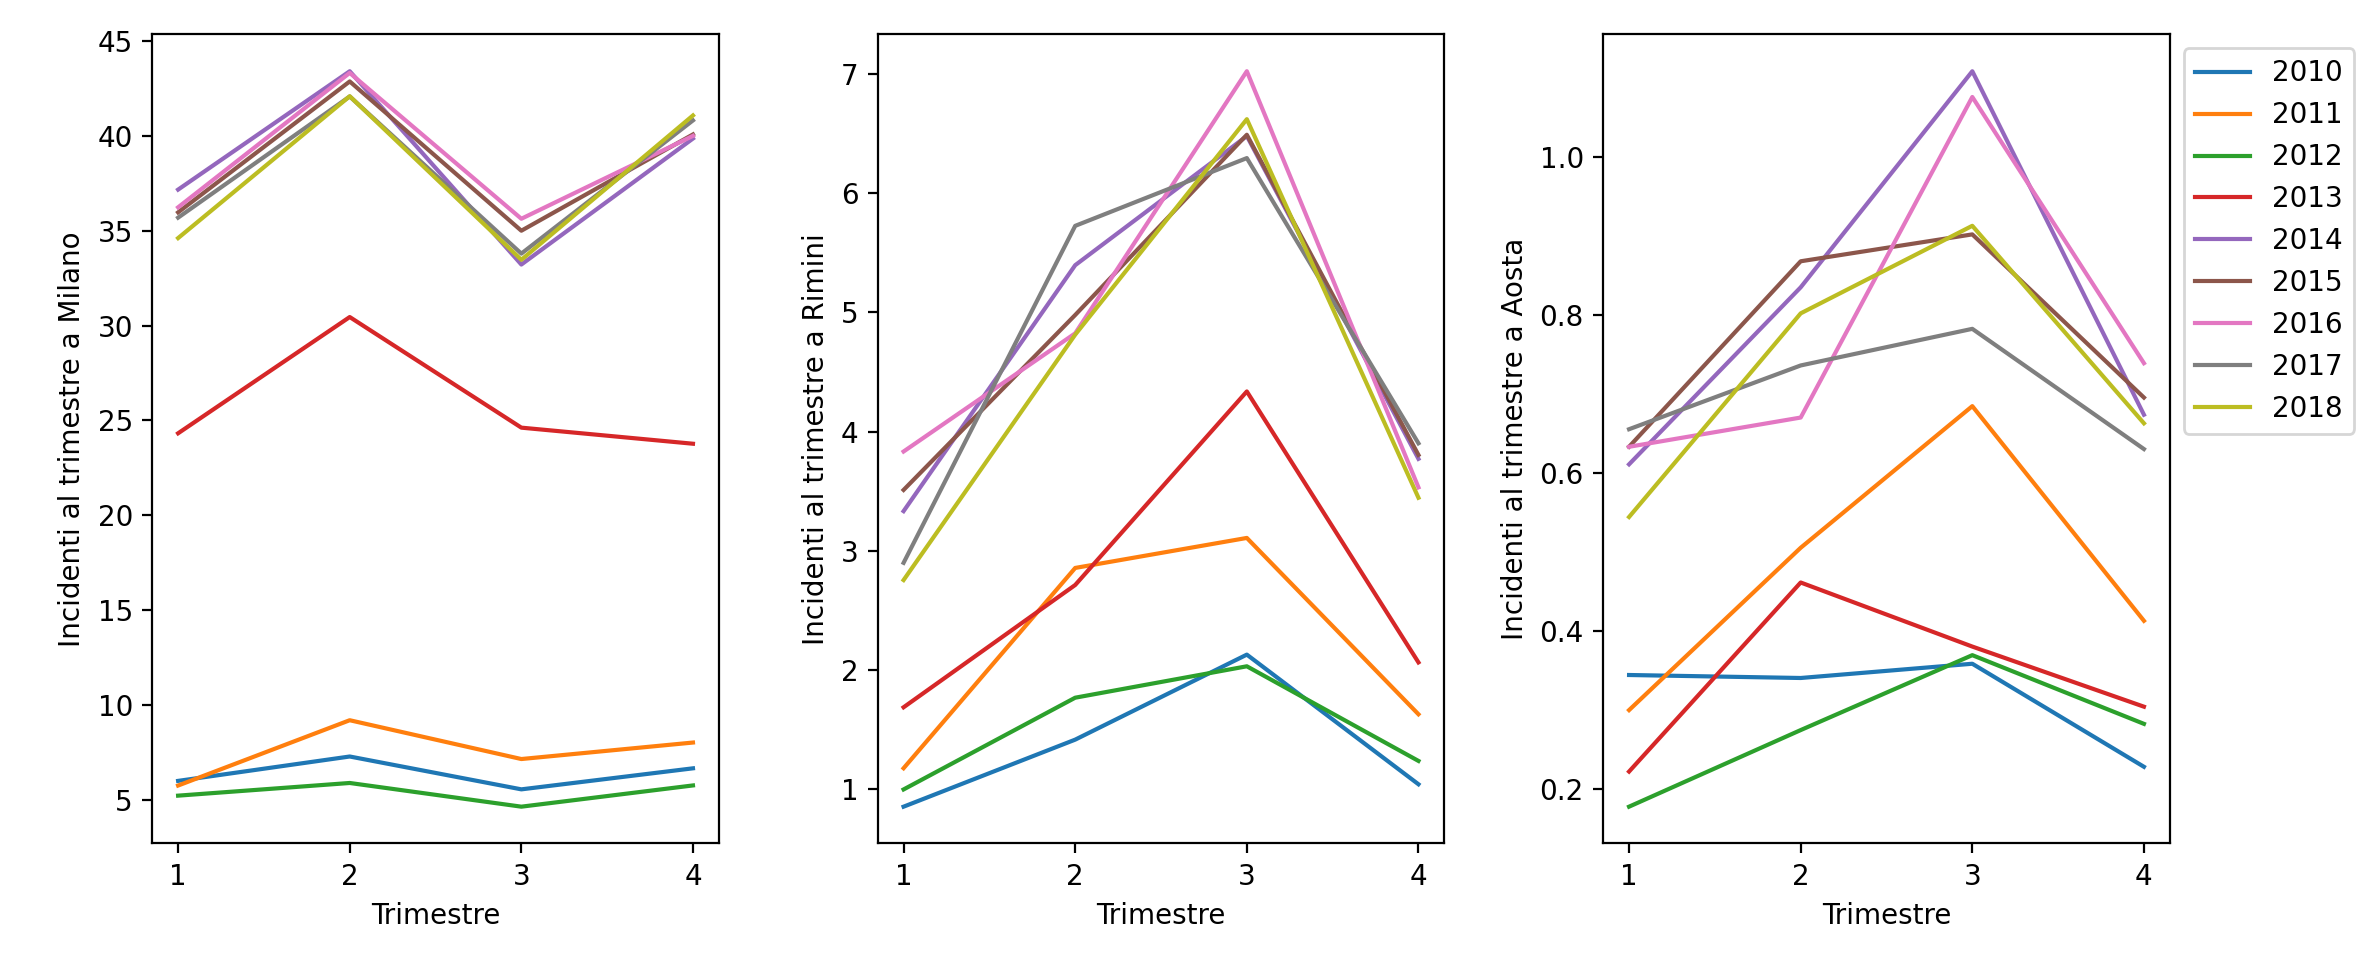
\includegraphics[width=\linewidth]{../src/incidenti/incidenti_senza_coords/mese_incidenti/trimestri_aosta_milano_rimini.png}
    \caption{Incidenti per trimestre in Valle d'Aosta, a Rimini e a Milano}
    \label{fig:aosta-rimini-milano-trimestre}
\end{figure}

In tutti i grafi nella figura \ref{fig:aosta-rimini-milano-trimestre}, 
si osserva, come già visto in precedenza, che dall'anno 2015 si ha un ampia crescita  
del numero di incidenti, probabilmente dovuta a un cambio di misurazione 
degli incidenti. 

Per quanto riguarda Rimini e Aosta, si osservano varie similitudini in quasi 
tutte le annate. In particolare si osserva un basso numero di incidenti 
durante il primo trimestre, e un incremento di sinistri durante il terzo trimestre.
D'altra parte, a Milano, si ha la tendenza opposta, con maggior numero di 
incidenti nel secondo trimestre, e un abbassamento durante il primo 
e terzo trimestre, soprattutto con l'aumento della taglia del campione, 
a partire dal 2015.

Ciò che è possibile dedurre, è che a Milano il numero di incidenti decresce 
nel terzo trimestre in concordanza con le partenze per le vacanze, mentre nelle 
altre località raffigurate, avviene la tendenza opposta poichè 
queste sono spesso mete feriali.

Sarebbe interessante conoscere l'esistenza di località di vacanza preferite, 
o se queste cambino il base all'anno. 
Si tenterà di rispondere a queste domande nei capitoli successivi.

%\clearpage
\section{Dati Istat su tipi di incidenti e incroci}

Riguardo i dati sulla località degli incidenti e sul tipo di incrocio, 
sarebbe interessante sapere se esistano tipologie di sinitri che accadono 
con più frequenza di altre. 
Un'altra questione potrebbe essere se, tra queste tipologie, il numero di feriti 
sia comparabile o se alcuni tipi di incidenti siano più pericolosi di altri.

%\clearpage
\subsection{Le tipologie di incidenti più frequenti}

Per rispondere alla prima delle domande poste nell'introduzione, è possibile, 
utilizzando i dati a disposizione, contare la frequenza di ogni categoria di incidente.

\begin{figure}
    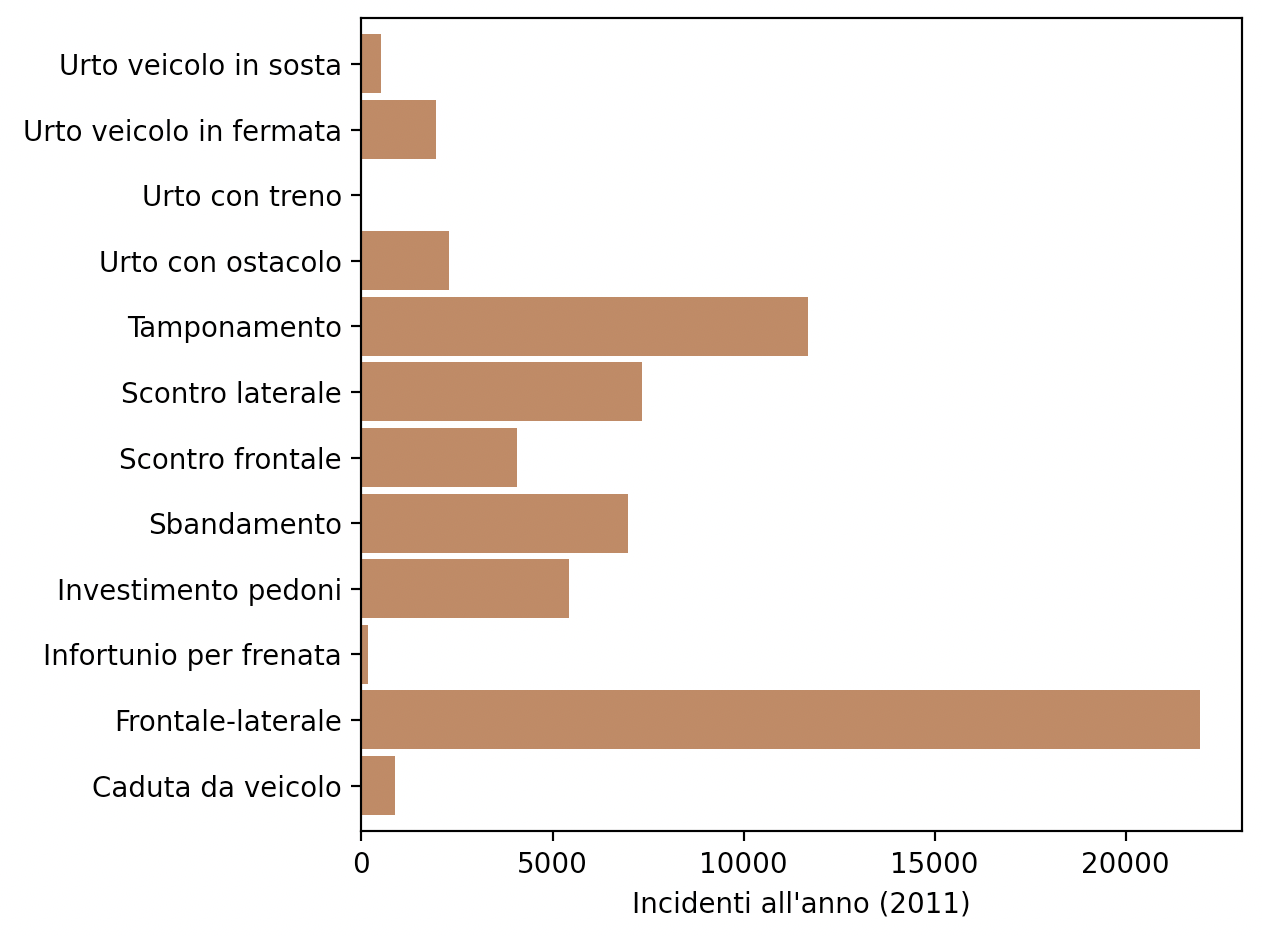
\includegraphics[width=\linewidth]{../src/incidenti/incidenti_senza_coords/localizzazione_incidente/tipo_incidente.png}
    \caption{Numero di incidenti divisi per tipologia}
    \label{fig:tipo-incidente}
\end{figure}

Nella figura \ref{fig:tipo-incidente} sono riportati gli incidenti più frequenti nel 2018.
In particolare sono molto frequenti scontri frontali, laterali e tamponamenti. 
La tipologia \columnstyle{frontali-laterali} è quella più rappresentata probabilmente per 
l'ampiezza della categoria, in quanto contiene tutte le sfumature di incidenti che non sono 
precisamente contatti frontali o precisamente laterali.

Prima di fare assunzioni errate, va detto che questo grafo, senza un constesto, 
non è molto utile, perchè il numero di incidenti di una categoria deve 
essere strettamente influenzato dalla tipo di strada e intersezione. 
Per esempio, si ha una probabilità bassa di essere coinvolti in un tamponamento 
se si sta guidando su un'autostrada, mentre il numero di casi aumenta se si viaggia 
su un viale con più semafori in serie.

Ciò che è possibile controllare, è se negli altri anni disponibili, le 
tipologie di intersezioni rimangano costanti o meno.
Le percentuali delle prime quattro categorie di incroci che provocano più sinistri 
sono riportate nella figura \ref{fig:rapporto-tipologie}: 

\begin{figure}
    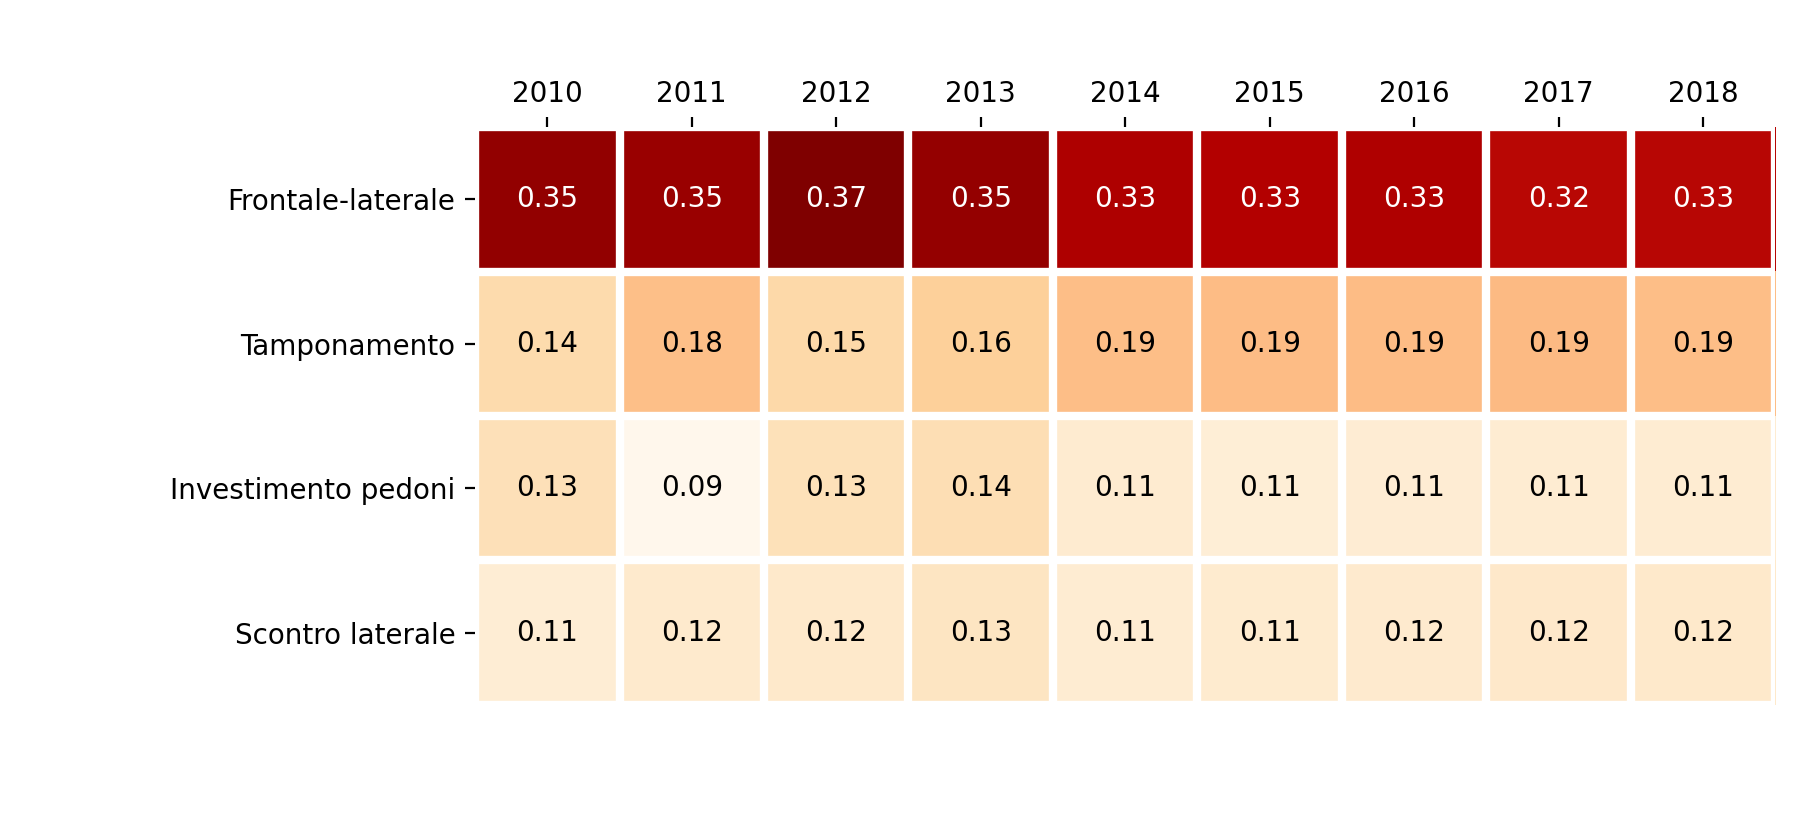
\includegraphics[width=\linewidth]{../src/incidenti/incidenti_senza_coords/localizzazione_incidente/rapporto_tipologie.png}
    \caption{Categorie più frequenti di incidente, divise per anno}
    \label{fig:rapporto-tipologie}
\end{figure}

Per tutte le annate disponibili, le prime due categorie di incidenti rimangono sempre 
le stesse, cioè \columnstyle{Scontro frontale-laterale} e \columnstyle{tamponamento}. 
Anche le percentuali corrispondenti restano molto simili, con la prima 
categoria sempre attorno al $35\%$ e la seconda attorno al $18\%$.

Nella terza categoria, d'altra parte, si inizano ad osservare delle differenze, 
poichè si alternano \columnstyle{investimento di pedoni} e \columnstyle{scontro laterale}, 
con percentuali simili, attorno al $12\%$.

Ciò che è possibile dedurre dalla figura \ref{fig:rapporto-tipologie}, è che non 
sembrano esistere fattori che influenzano quali tipi di sinistro 
vengano commessi maggiormente in un anno. 

Se si avessero a disposizione dei dati riguardanti il numero e il tipo 
di incroci in una località, sarebbe possibile giustificare 
la maggiore frequenza di sinistri di un tipo rispetto a un altro. 

\subsection{I tratti di strada più pericolosi}

Il dataset di incidenti Istat contiene informazioni riguardanti il tipo di 
intersezione nel quale è avvenuto l'incidente.
Sarebbe molto utile, anche in questo caso, avere il numero di incroci per tipo 
presenti in una certa località, per controllare se alcuni incroci siano più 
frequenti di altri.

Non avendo accesso a questo tipo di informazioni, si è utilizzato l'indice di 
mortalità per tipologia di sinistro, prendendo spunto dalla sintesi dello 
studio su incidenti stradali, eseguito da ACI \cite{ACI:2}.

Nel grafo sul lato sinistro della figura \ref{fig:tipo-intersezioni}, 
sono rappresentati gli incidenti in Italia nel 2018, divisi per tipologia 
di incrocio in cui sono avvenuti.
\todo{allineare}
\begin{figure}
    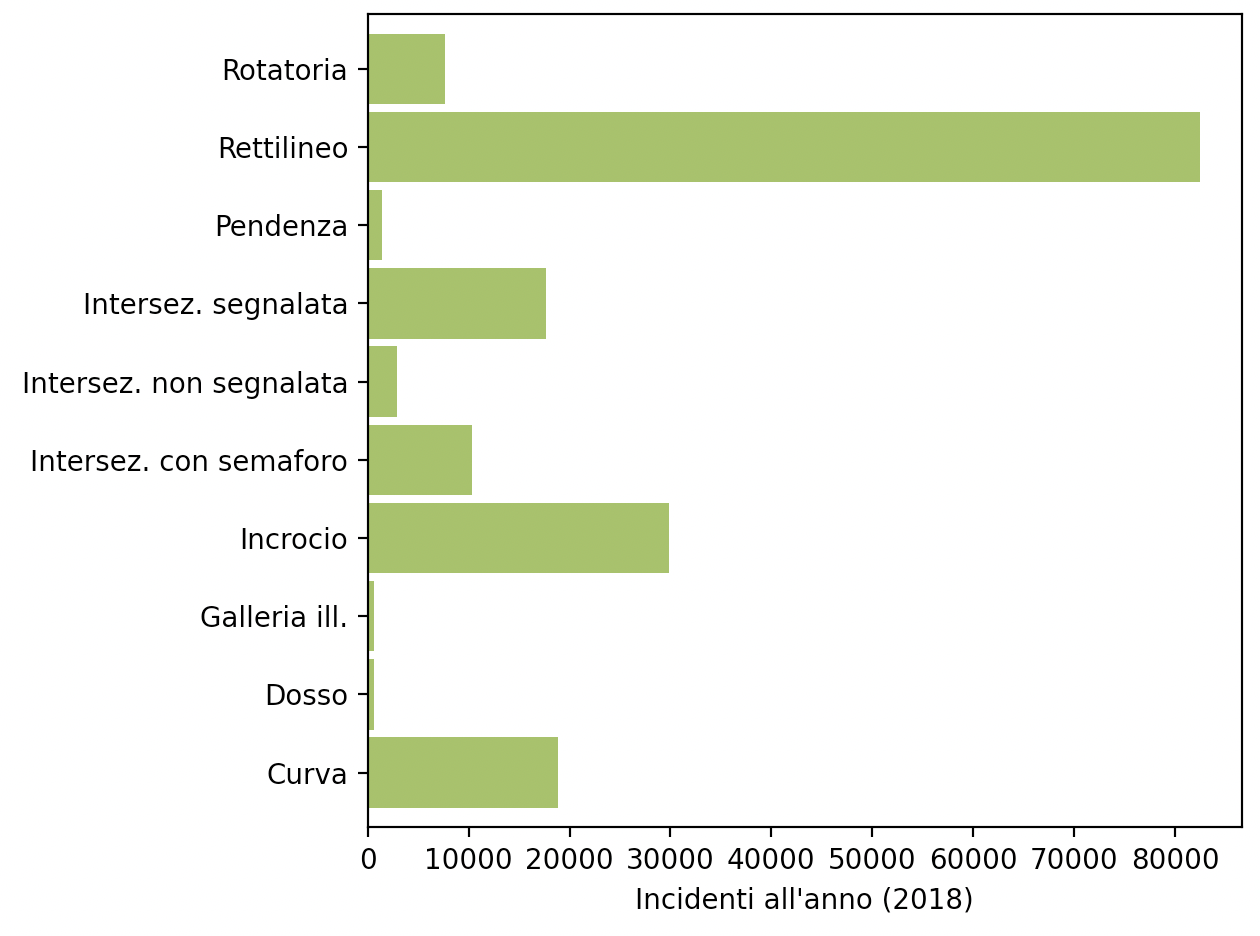
\includegraphics[width=0.5\linewidth]{../src/incidenti/incidenti_senza_coords/localizzazione_incidente/intersezioni.png}
    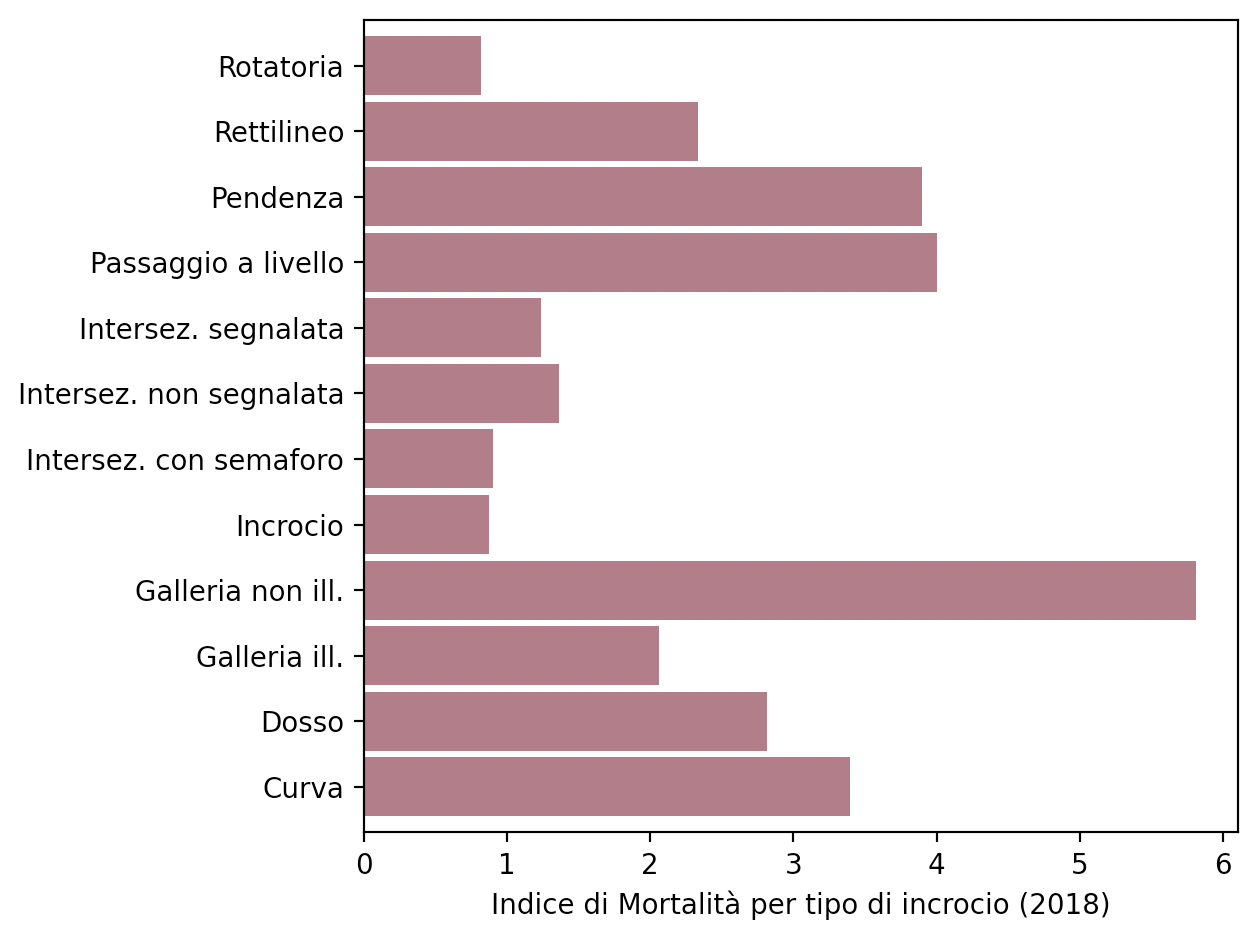
\includegraphics[width=0.5\linewidth]{../src/incidenti/incidenti_senza_coords/localizzazione_incidente/indice_mortalita.png}
    \caption{Percentuale di incidenti e rispettivo indice di mortalità per tipo di incrocio}
    \label{fig:tipo-intersezioni}
\end{figure}

I risultati sono piuttosto eterogenei, con la maggior parte dei sinistri 
localizzati lungo rettilinei, incroci e curve. 
\'E possibile ipotizzare che, viste le alte velocità raggiunte dalle automobili 
lungo i rettilinei, i risultati calcolati siano corretti, e questa categoria sia 
particolarmente pericolosa.
Tuttavia è più probabile che il numero di incidenti di questa tipologia sia dovuto 
all'alta frequenza di tratti di strada dritti.

Ulteriore conferma di questa teoria, è data dall'indice di mortalità per tipologia di incrocio, 
riportato nel grafo destro dell'immagine \ref{fig:tipo-intersezioni}, e calcolato tramite le 
formule sottostanti. 

\begin{center}
    $Indice\_Mortalita\_Strada\_X = \displaystyle \frac{Numero\_Morti\_Strada\_X}{Numero\_Incidenti\_Strada\_X} * 100$ 
\end{center}

\begin{center}
    $Indice\_Feriti\_Strada\_X = \displaystyle \frac{Numero\_Feriti\_Strada\_X}{Numero\_Incidenti\_Strada\_X} * 100$ 
\end{center}

Questo indicatore mostra come, nonostante i rettilinei siano le zone in cui 
avvengono più frequentemente incidenti, questi non siano i tratti di 
strada più pericolosi. 

Nella tabella sottostante sono riportati i valori, sia dell'indice di mortalità, 
sia dell'indice di feriti per tipologia di strada in cui è avvenuto l'incidente.

\begin{center}
    \def\arraystretch{1.5}%  
    \begin{tabular}{ |c|c|c| } 
    \hline
    Tipo di Incrocio & Indice Mortalità & Indice Feriti \\ 
    \hline
    \rowcolor{TableGray}
    Incrocio                & 0.88 & 143.10 \\
    Rotatoria               & 0.82 & 127.22 \\
    \rowcolor{TableGray}
    Intersez. segnalata     & 1.24 & 142.14 \\
    Intersez. con semaforo  & 0.9 & 147.05 \\
    \rowcolor{TableGray}
    Intersez. non segnalata & 1.36 & 139.97\\
    Passaggio a livello     & 4.0 & 134.67\\
    \rowcolor{TableGray}
    Rettilineo              & 2.33 & 138.94\\
    Curva                   & 3.39 & 145.26\\
    \rowcolor{TableGray}
    Dosso                   & 2.82 & 156.49\\
    Pendenza                & 3.9 & 134.10\\
    \rowcolor{TableGray}
    Galleria ill.           & 2.06 & 165.87\\
    Galleria non ill.       & 5.81 & 132.59\\
    \hline
    \end{tabular}
\end{center}

Per controllare la validità degli indici calcolati, si è ricavata la correlazione 
tra indice di mortalità, feriti e tra questi ultimi e il numero di incidenti per 
luogo.
I valori sono riportati nella tabella sottostante: 

\begin{center}
    \def\arraystretch{1.5}%  
    \begin{tabular}{ |c|c| }
        \hline
        \rowcolor{TableGray}
        Tra morti e feriti      & 0.96 \\ 
        Tra incidenti e feriti  & 0.99 \\
        \rowcolor{TableGray}
        Tra incidenti e morti   & 0.96 \\
        \hline
    \end{tabular}
\end{center}

Ne risulta che tutti gli insiemi siano linearmente correlati tra loro. 
Dalla tabella contenente l'indice di feriti, non è possibile dedurre molto, 
in quanto questo indicatore è molto simile tra tutte le categorie. 
Tuttavia, il minimo indice di mortalità e di feriti, si ha nella stessa categoria, 
la rotatoria, informazione potrebbe essere molto utile durante la realizzazione di nuovi 
incroci.

Per quanto riguarda invece, l'indice di mortalità, è chiaro che sia più alto 
per categorie di incidenti che avvengono ad alte velocità, come vicino a dossi, 
curve e gallerie, rispetto a tratti di strada, come incroci e semafori, 
dove le automobili stanno ripartendo.

%\clearpage
\subsection{Le tipologie di incidenti che provocano più feriti}

Il dataset Istat contiene informazioni riguardanti il numero di persone coinvolte 
in incidenti, in particolare l'età, il sesso e l'esito. 
Per quest'ultimo campo, si intende lo stato di salute del passeggero 
dopo l'incidente, che può essere: incolume, ferito, morto entro 24 ore o morto entro un mese.
Sarebbe interessante controllare se esistano tipologie di incidenti che provocano 
un maggior numero di feriti.

\begin{figure}
    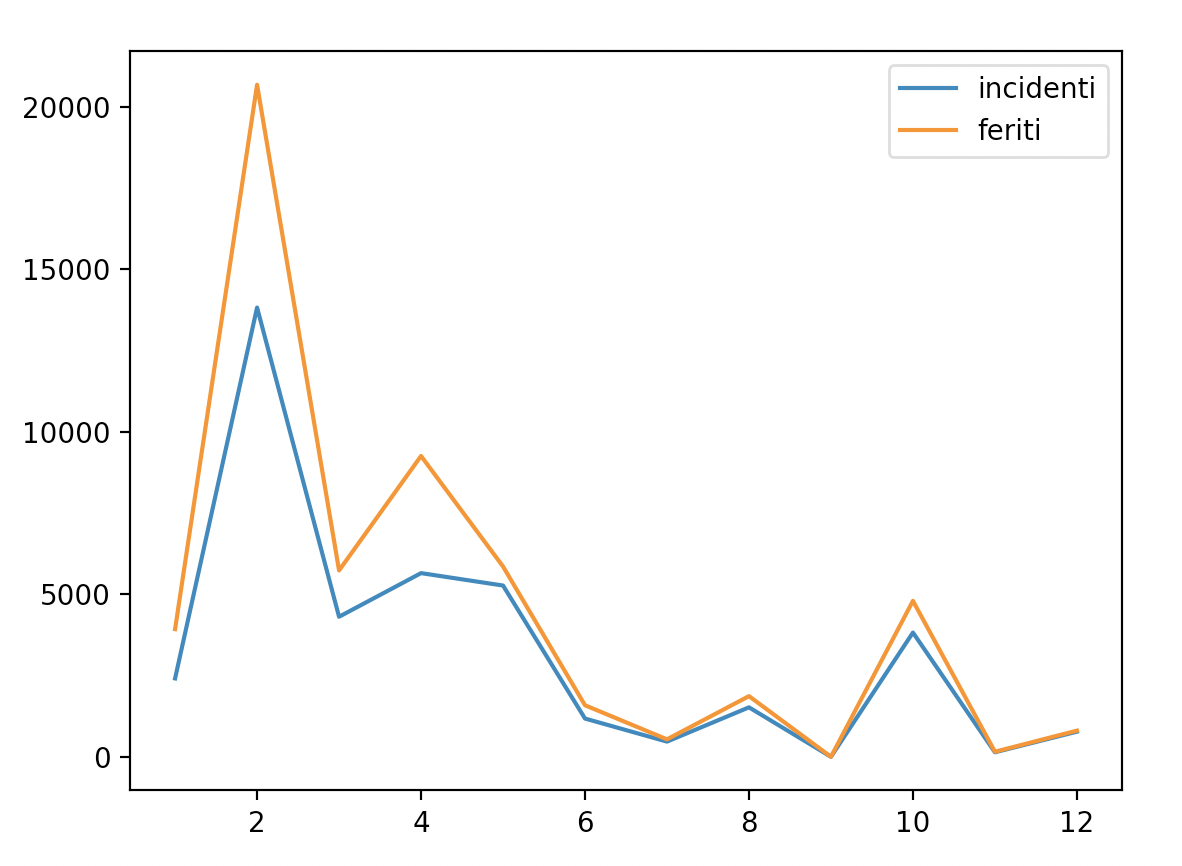
\includegraphics[width=\linewidth]{../src/incidenti/incidenti_senza_coords/natura_incidente/natura_incidente.png}
    \caption{Numero di feriti in base alla natura dell'incidente}
    \label{fig:numero-feriti}
\end{figure}

Dalla figura \ref{fig:numero-feriti} è possibile ipotizzare l'esistenza di tipologie 
di sinistri che favoriscono la presenza di un solo ferito, come gli sbandamenti. 
Si arriva a questa conclusione perchè la colonna di questo tipo di incidente, è tra 
le più alte di quelle del primo gruppo (un solo ferito), 
mentre nel secondo gruppo (due feriti), la stessa categoria è tra i valori 
più bassi.
Al contrario, le colonne corrispondenti al \columnstyle{tamponamento}, sono molto alte 
per ognuno dei quattro gruppi, il che fa pensare che semplicemente avvenga un alto numero 
di sinistri di questo tipo.

Le percentuali di osservazione degli incidenti nel grafo \ref{fig:numero-feriti} sono 
riportate nella tabella sottostante\footnote{La somma delle percentuali dei tipi di 
incidenti dovrebbe ammontare a 1, ma sono state riportate solo quattro categorie 
interessate, e non tutte.}: 

\begin{center}
    \def\arraystretch{1.5}%  
    \begin{tabular}{ |c|c| } 
    \hline
    Incidente & Percentuale del tipo \\ 
    \hline
    \rowcolor{TableGray}
    Sbandamento       & 0.097 \\
    Tamponamento      & 0.143 \\
    \rowcolor{TableGray}
    Scontro frontale  & 0.061 \\
    Urto con ostacolo & 0.039 \\
    \hline
    \end{tabular}
\end{center}

Avendo a disposizione il numero di incidenti per categoria, è possibile capire 
se il comportamento visibile nel grafo sia dovuto al numero di sinistri, o alla 
pericolosità del tipo di scontro. 

\begin{figure}
    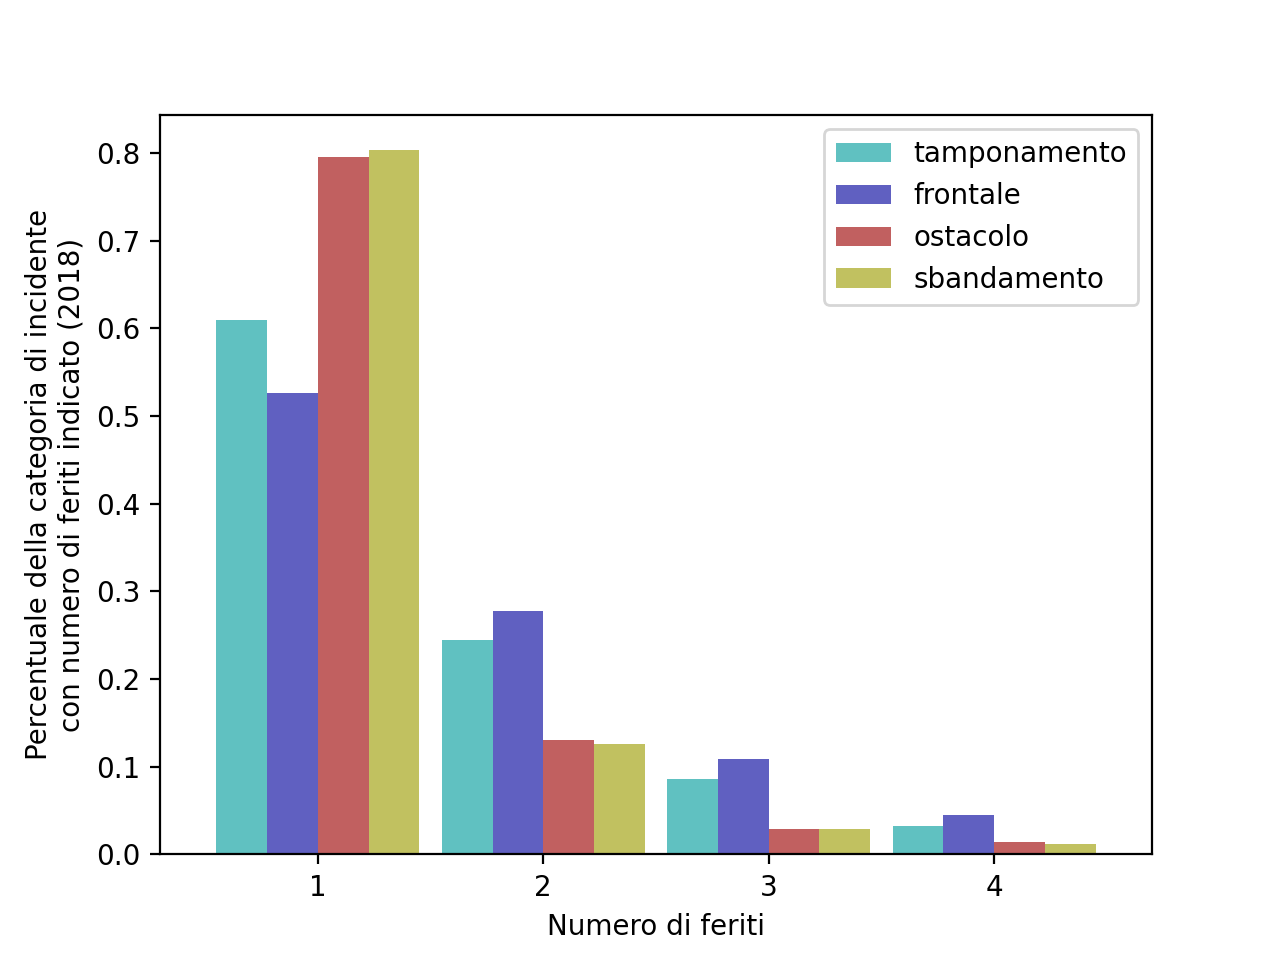
\includegraphics[width=\linewidth]{../src/incidenti/incidenti_senza_coords/natura_incidente/perc_natura_incidente.png}
    \caption{Frequenza del tipo di incidente con numero di feriti, diviso per la percentuale di incidenti della rispettiva categoria}
    \label{fig:perc-numero-feriti}
\end{figure}

La figura \ref{fig:perc-numero-feriti} mostra la frequenza di incidenti con un dato numero 
di feriti, divisa per la percentuale di sinistri della categoria interessata.

Avendo a disposizione un indice di incidenti, corretto in base al volume della categoria 
di incidente, si osserva come alcune tipologie, come \columnstyle{urto con ostacolo} 
e \columnstyle{sbandamento}, favoriscano una sola persona ferita, mentre altre, 
come i \columnstyle{tamponamenti} e gli \columnstyle{scontri frontali}, presentino 
una maggiore percentuale di scontri con più di un ferito.

%\clearpage
\subsection{Incroci che favoriscono incidenti con pedoni}

Il dataset Istat fornisce varie informazioni riguardanti i pedoni coinvolti in un 
incidente, tramite le colonne \columnstyle{pedone\_morto\_sesso}, 
\columnstyle{pedone\_ferito\_sesso},\columnstyle{pedone\_morto\_età} e 
\columnstyle{pedone\_ferito\_età}.

Si potrebbe controllare l'esistenza di tipologie di incrocio che 
coinvolgono un alto numero di persone a piedi. 

\begin{figure}
    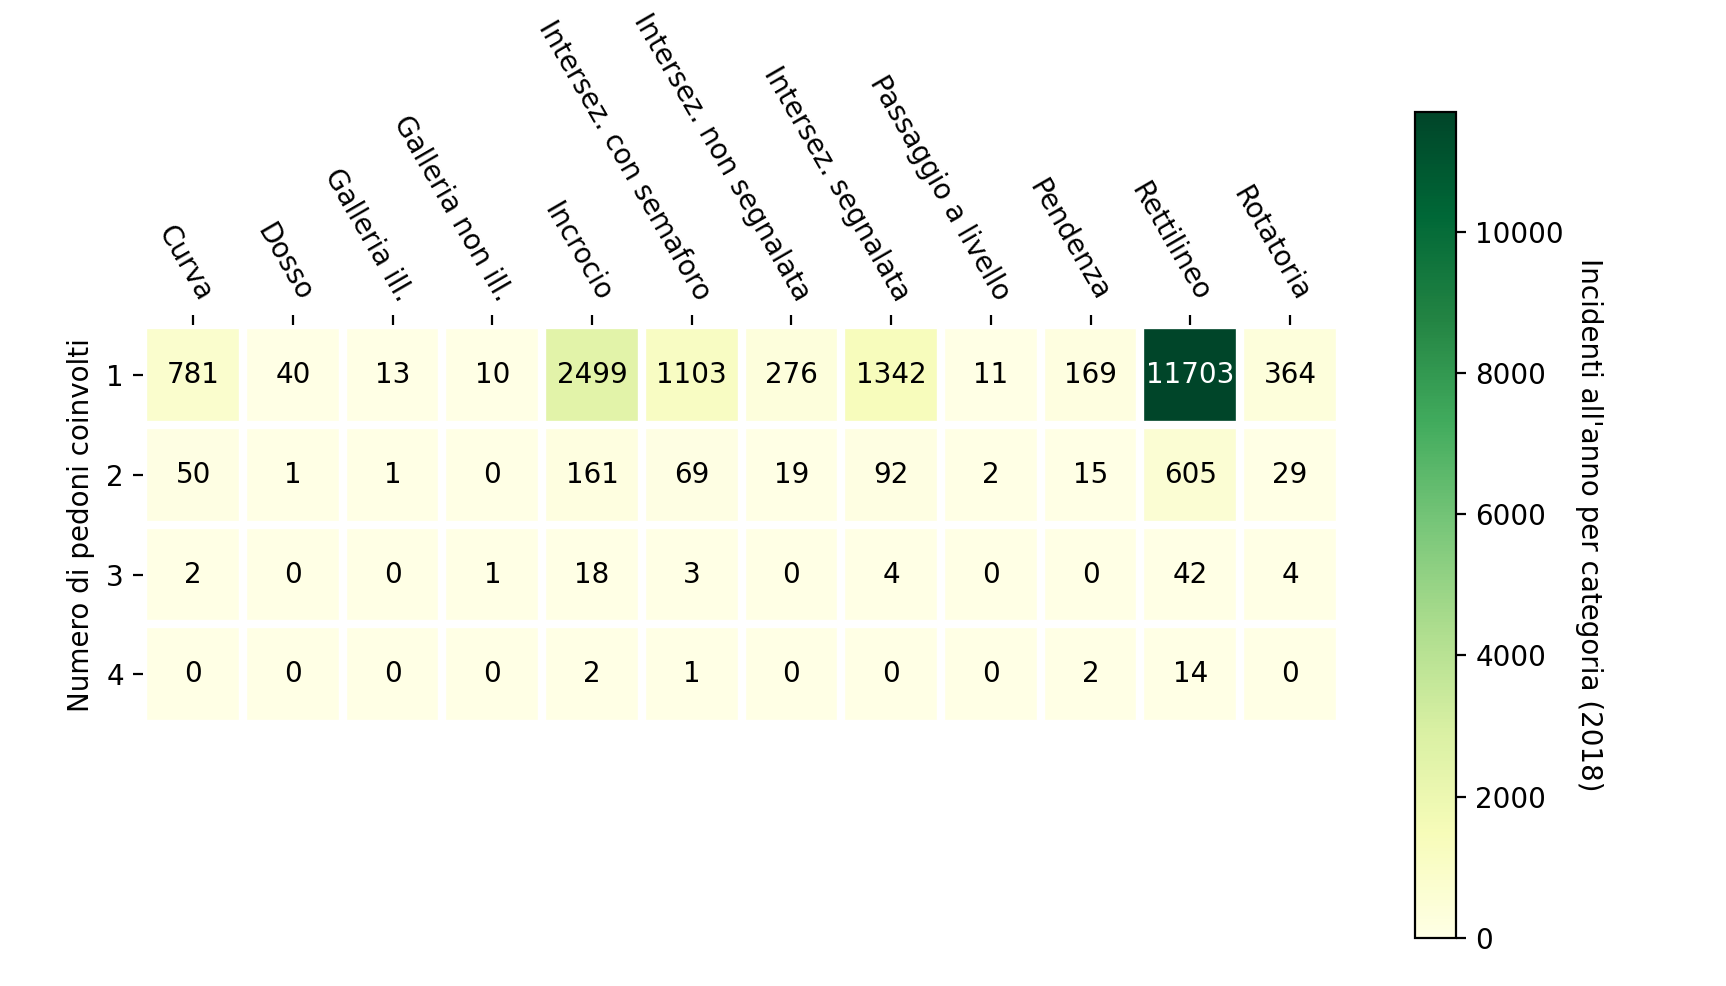
\includegraphics[width=\linewidth]{../src/incidenti/incidenti_senza_coords/pedoni/pedoni_incroci.png}
    \caption{Tipologia di intersezioni e pedoni coinvolti}
    \label{fig:pedoni-intersezioni}
\end{figure}

La figura \ref{fig:pedoni-intersezioni} mostra il numero di incidenti, 
ordinati in base alla tipologia di intersezioni in cui sono avvenuti 
e al numero di persone coinvolte.

Come si era già visto nel grafo\ref{fig:tipo-intersezioni}, nella nuova 
figura spicca un alto numero di rettilinei. 
Analogamente all'analisi precedente, si è inclini a pensare che il valore 
elevato di questa categoria sia dovuto dovuto all'alto 
numero di tratti di strada dritti, tuttavia, se si confrontano le due immagini, 
il numero di incidenti su rettilineo è quasi cinque 
volte il valore della seconda posizione.

Questo alto numero di sinistri fa pensare che esista un qualche fattore 
che comporti maggiore coinvolgimento di pedoni lungo rettilinei come, per 
esempio, l'alta velocità dei veicoli.

\begin{figure}
    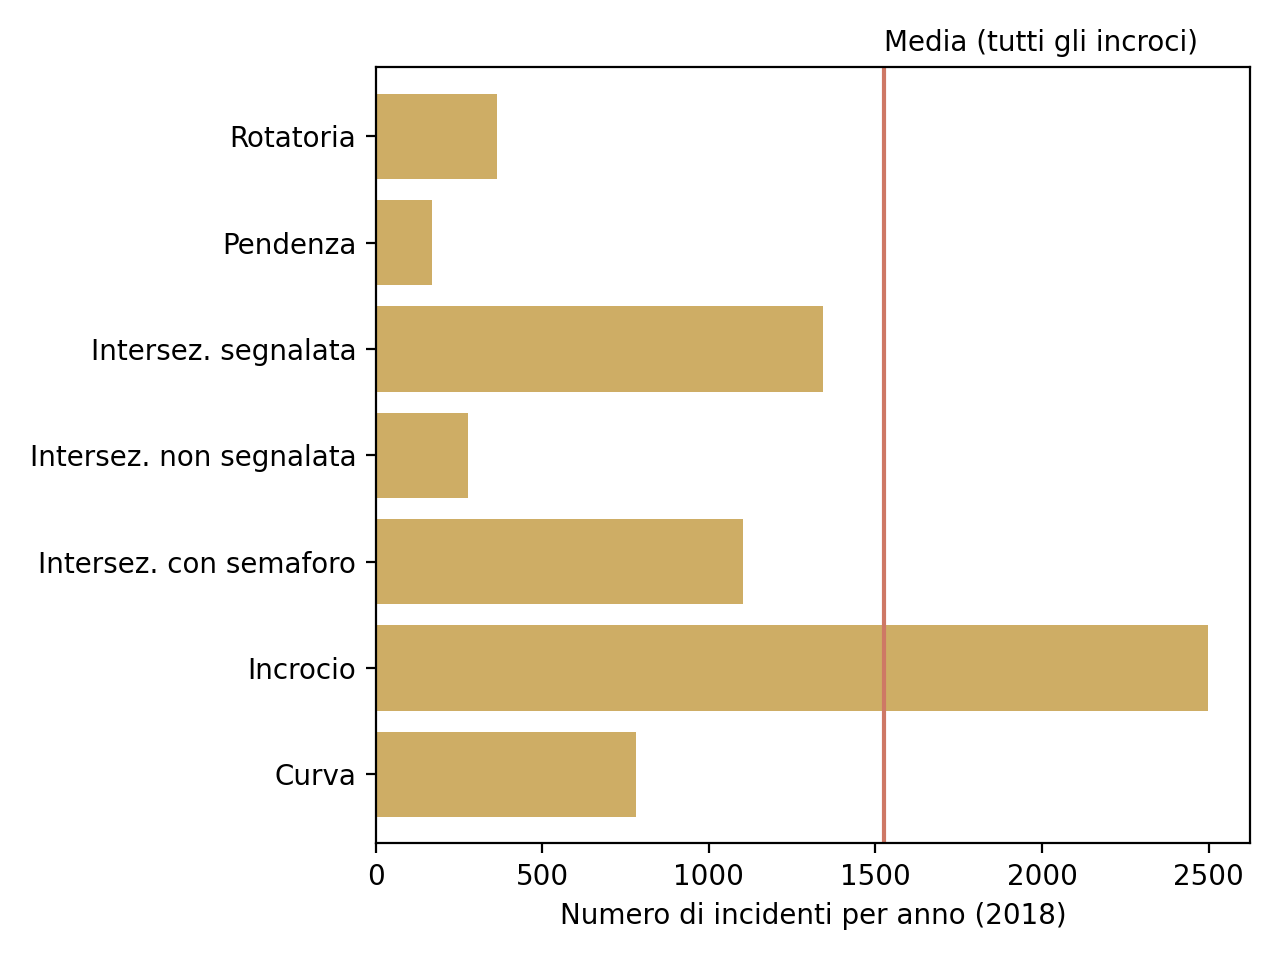
\includegraphics[width=\linewidth]{../src/incidenti/incidenti_senza_coords/pedoni/pedoni_no_rett.png}
    \caption{Tipologia di intersezioni e pedoni coinvolti, ignorando le categorie con valori più bassi}
    \label{fig:pedoni-no-rett}
\end{figure}

In figura \ref{fig:pedoni-no-rett} sono state escluse le categorie con minore 
valore\footnote{Sono state rimosse tutte le categorie con valore minore di 
150 incidenti all'anno}, 
in particolare \columnstyle{Dosso}, \columnstyle{Galleria ill.}, 
\columnstyle{Galleria non ill.,} e \columnstyle{Passaggio a livello}.
Il grafo ottenuto è più bilanciato, con \columnstyle{incroci} e 
\columnstyle{intersezioni non segnalate} che spiccano come tipi di strada con 
maggiore coinvolgimento di pedoni, ovviamente dopo \columnstyle{rettilineo}, 
e le restanti categorie non troppo distanti.

Va specificato che il grafo \ref{fig:pedoni-no-rett} è stato realizzato utilizzando, 
nell'asse delle ascisse, una scala logaritmica, poichè il numero di pedoni coinvolti 
su rettilineo è un ordine di grandezza maggiore rispetto alla media.

A differenza della precedente analisi sui tratti di strada più pericolosi, 
ignorando momentaneamente i rettilinei, l'immagine dipinta è molto diversa.
In questo caso, non si può più dire che i tratti più pericolosi siano quelli 
che favoriscono alte velocità, ma sembra che il maggior numero di pedoni 
siano coinvolti in incroci e zone in cui la visibilità è ostruita in 
qualche modo, come nelle curve.

%\clearpage
\subsection{Età dei pedoni coinvolti in incidenti}

\'E scontato che, se coinvolto in un incidente, un ventenne non ha la stessa 
probabilità di essere ferito rispetto a un pedone che ha settanta anni.
La domanda che sorge spontanea è se sia possibile osservare questo comportamento 
utilizzando i dati a disposizione.

Per prima cosa, si sono utilizzati i campi 
\columnstyle{pedone\_ferito\_età}\footnote{Nel dataset sono presenti quattro colonne per 
annotare l'età dei pedoni coinvolti.} 
per creare un grafo in cui sia visibile il numero di passanti feriti e morti, 
divisi per le categorie disponibili.

\begin{figure}
    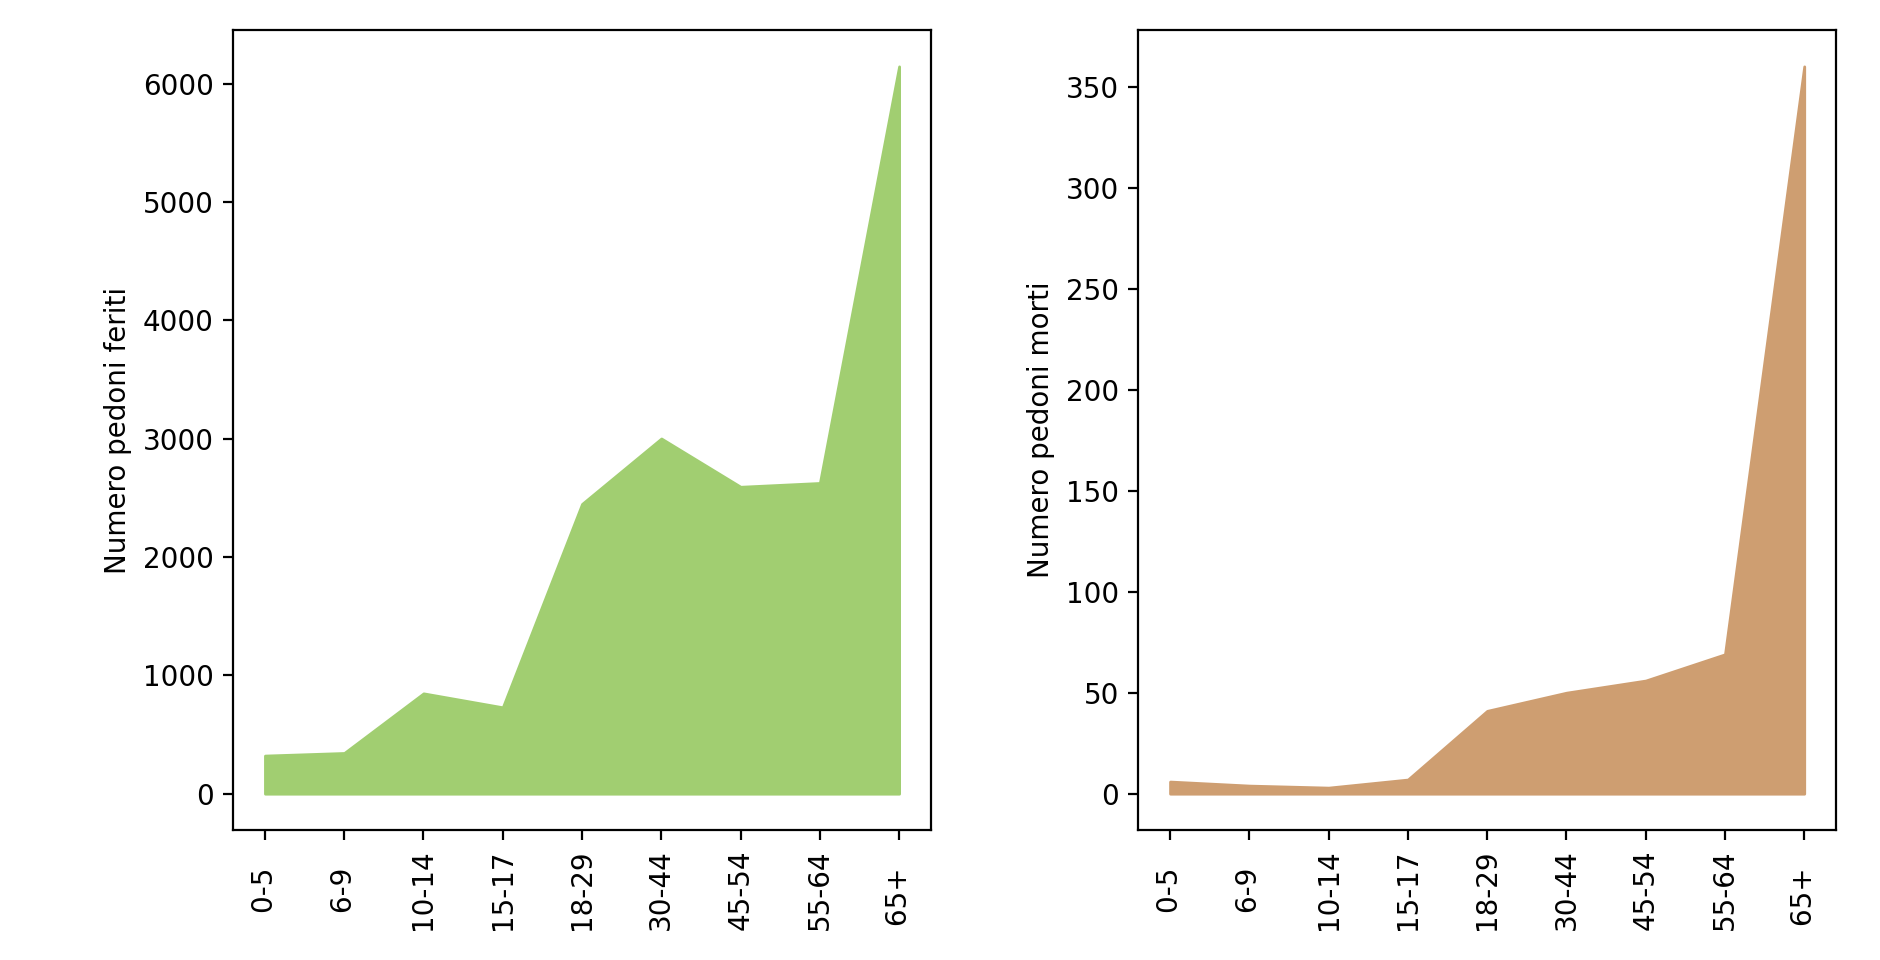
\includegraphics[width=\linewidth]{../src/incidenti/incidenti_senza_coords/pedoni/eta_pedoni_iniziale.png}
    \caption{Frequenze di coinvolgimento di pedoni in incidenti per fascia di età}
    \label{fig:eta-pedoni-iniziale}
\end{figure}

Dal grafo \ref{fig:eta-pedoni-iniziale} si osserva come la fascia di età più colpita 
sia quella dei \columnstyle{65+} anni, tuttavia esiste un secondo picco, nel grafo dei 
pedoni feriti, che comprende le persone tra i trenta e cinquantaquattro anni di età.

Non tutte queste fasce, però, contengono lo stesso numero di anni di età, 
per esempio \columnstyle{30-44} contiene quindici anni, mentre 
\columnstyle{18-20} ne contiene solo due.

\begin{code}[language=Python]
numero_anni = np.array([5, 5, 5, 3, 10, 15, 10, 10, 20])

pedoni_feriti_vals = pedoni_feriti.values / numero_anni
pedoni_morti_vals = pedoni_morti.values / numero_anni
\end{code}

\begin{figure}
    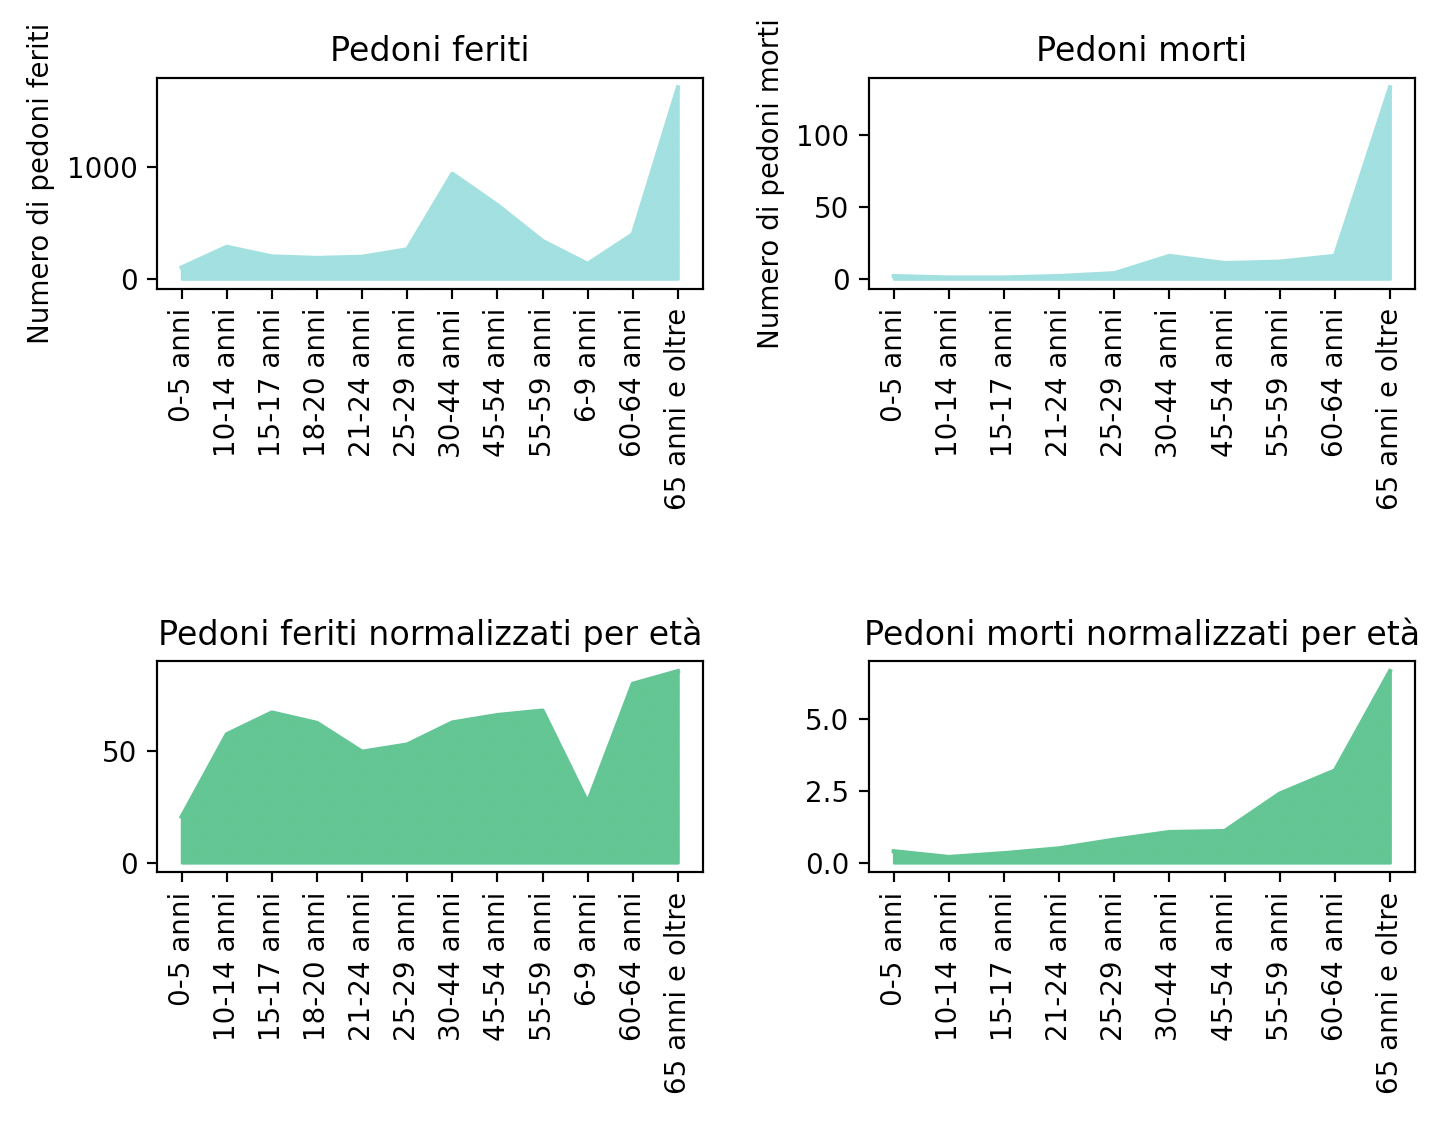
\includegraphics[width=\linewidth]{../src/incidenti/incidenti_senza_coords/pedoni/eta_pedoni.png}
    \caption{Fasce di età dei pedoni coinvolti in incidenti, normalizzate per numero di anni 
    presenti nella categoria}
    \label{fig:eta-pedoni}
\end{figure}

Se si normalizza per anni contenuti in ogni fascia, ipotizzando un numero 
costante di persone di ogni età\footnote{La normalizzazione tiene conto 
che la fascia di età \columnstyle{65+} valga venti anni.}, 
si ottiene un grafo, visibile in figura \ref{fig:eta-pedoni}. 
Per quanto riguarda i pedoni feriti, questa rappresentazione è molto differente.
Ignorando gli individui più giovani, tutte le altre fasce sono coinvolte 
in modo omogeneo, con un picco nella categoria \columnstyle{65+ anni}.
D'altra parte, il grafo destro, contenente i morti per fascia di età, 
non subisce un grande cambiamento, mantenendo il punto di massimo nei 
pedoni più anziani.

Non è detto, tuttavia, che in Italia il numero di individui con 
la stessa età sia costante, anzi, le percentuali di individui per fascia, 
trovate sul sito Tuttitalia \cite{TUTTITALIA:1}, riportate nella tabella 
sottostante, non sono particolarmente omogenee: 

\begin{center}
    \def\arraystretch{1.5}%  
    \begin{tabular}{ |c|c| } 
    \hline
    Età & Percentuale Popolazione \\ 
    \hline
    \rowcolor{TableGray}
    0-5     & 3.9 \% \\ 
    6-9     & 4.5 \% \\
    \rowcolor{TableGray}
    10-14   & 4.8 \% \\
    15-17   & 3.1 \% \\
    \rowcolor{TableGray}
    18-20   & 2.8 \% \\ 
    21-24   & 4   \% \\
    \rowcolor{TableGray}
    25-29   & 5.3 \% \\
    30-44   & 19  \% \\
    \rowcolor{TableGray}
    45-54   & 18.2\% \\ 
    55-59   & 7.3 \% \\
    \rowcolor{TableGray}
    60-64   & 6.4 \% \\
    65$+$   & 19.3\% \\
    \hline
    \end{tabular}
\end{center}

Visto che gli insiemi di popolazione del sito e quelle del dataset Istat non coincidono, 
si è dovuto, in alcuni casi sommare, in altri suddividere, i dati di Tuttitalia.
Nel secondo caso, si è necessario stimare la percentuale di popolazione con 
determinata età, in quanto si deve dividere una fascia.
Un esempio è la categoria dei \columnstyle{15-19} anni, 
i dati Istat hanno un insieme per \columnstyle{15-17} anni e un altro per 
\columnstyle{18-29} anni, 
è dunque necessario spostare i diciotto e i diciannovenni dalla prima alla 
seconda fascia. 
In questi casi, si è semplicemente assunto che il numero di individui sia omogeneamente 
diviso per età, cioè in \columnstyle{15-19 anni} si abbia lo stesso numero di 
quindicenni e sedicenni.
Seguendo questa logica, per spostare i due anni di età nella categoria successiva, 
è opportuno dividere la cardinalità\footnote{Il numero di elementi presenti nell'insieme.} 
dell'insieme \columnstyle{15-19} per cinque e moltiplicarlo per due. 
Il risultato ottenuto va aggiunto alla fascia \columnstyle{18-29}.

\begin{code}
correct_order =         ['0-5  ', '6-9  ', '10-14', '15-17', '18-29', '30-44', '45-54', '55-64','65+  ']
perc_fascia = np.array( [3.9, 4.5, 4.8, 3.1, 12.1, 19, 18.2, 13.7, 19.3]) / 100

pedoni_feriti_vals = pedoni_feriti.values / perc_fascia
pedoni_morti_vals = pedoni_morti.values / perc_fascia
\end{code}

\begin{figure}
    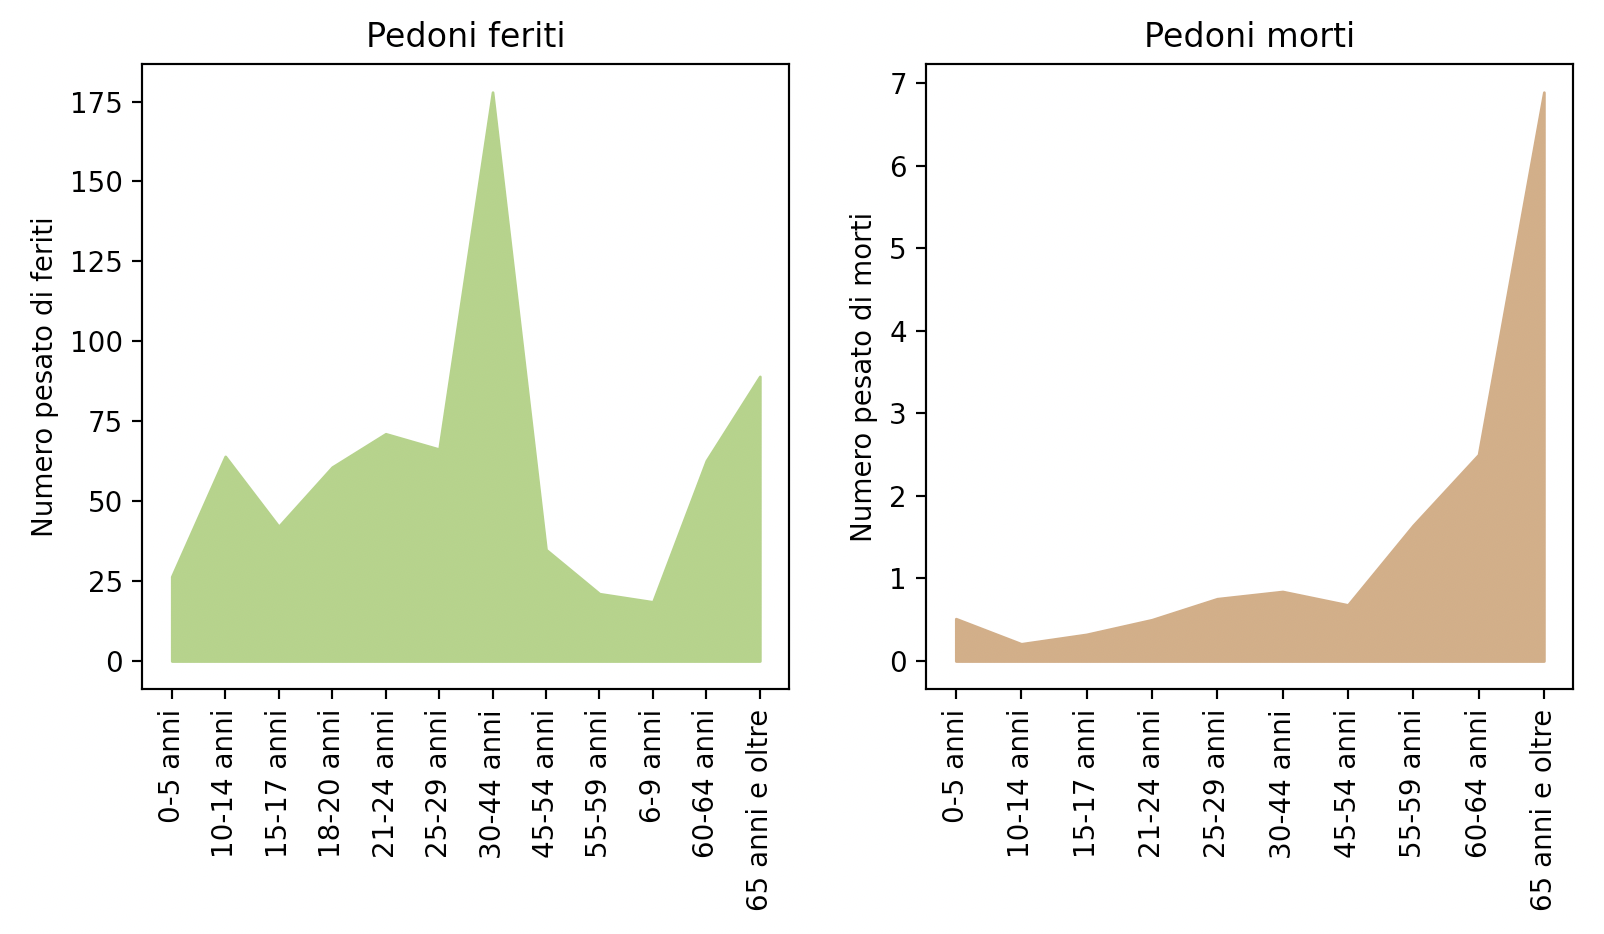
\includegraphics[width=\linewidth]{../src/incidenti/incidenti_senza_coords/pedoni/eta_pedoni_norm.png}
    \caption{Fasce di età dei pedoni coinvolti in incidenti, normalizzate tramite percentuale di popolazione}
    \label{fig:eta-pedoni-norm}
\end{figure}

Una volta aver corretto l'immagine precendente, si ottiene la figura \ref{fig:eta-pedoni-norm} 
dove, soprattutto nel grafo di destra, è presente una curva particolarmente alta 
nelle fasce più anziane, e un secondo picco nella categoria \columnstyle{18-29 anni}.
Anche nel grafo di sinistra è presente la stessa impennata in corrispondenza 
della seconda fascia, mentre nei \columnstyle{65+} non 
risulta particolarmente alta.

Si può speculare che l'incremento di morti nelle fasce più anziane, sia dovuto al 
fatto che questi ultimi siano più propensi all'essere feriti in un incidente. 
Le categorie centrali, in particolare \columnstyle{18-29 anni}, una volta 
aggiustati i calcoli per popolazione, sembrano essere comunque quelle più 
coinvolte in sinistri.

\subsection{Età dei conducenti coinvolti in incidenti}

Avendo a disposizione le informazioni riguardanti l'età del conducente del 
veicolo che ha causato l'incidente, è possibile controllare se esistono fasce di 
età che provocano un numero di sinistri particolarmente alto.

\begin{figure}
    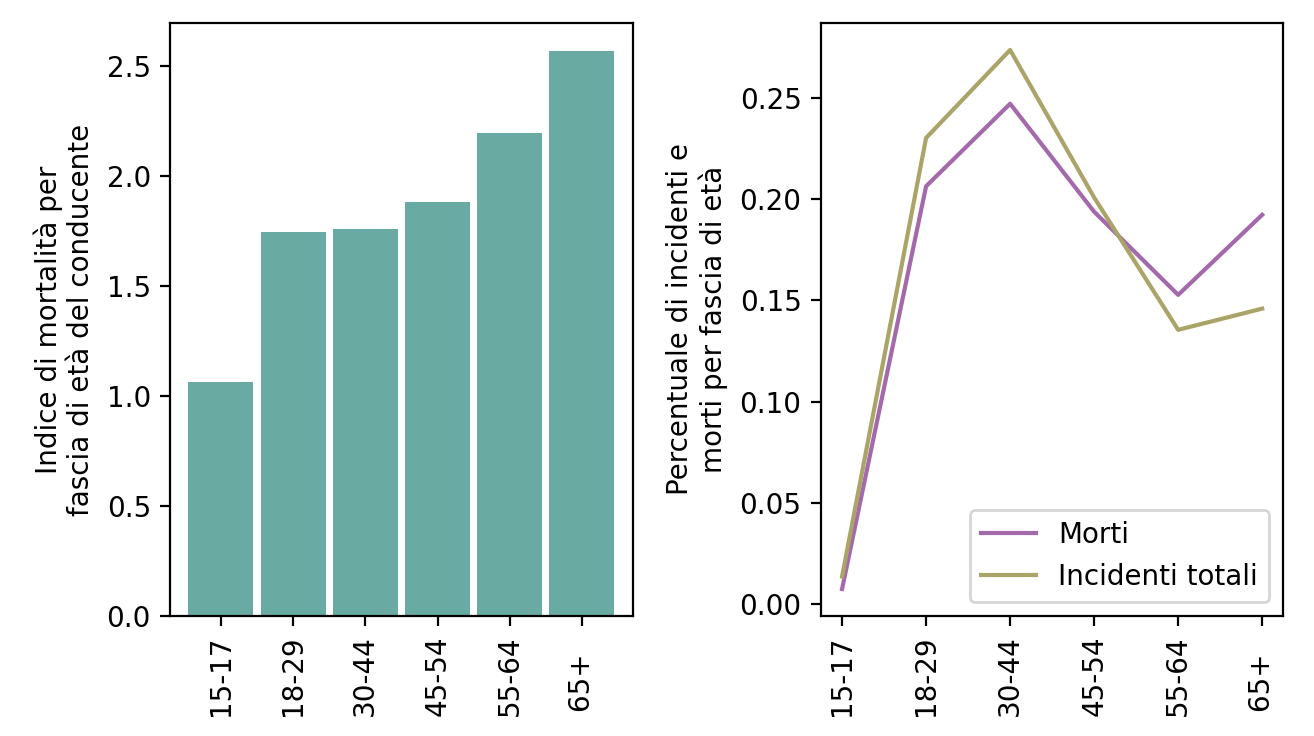
\includegraphics[width=\linewidth]{../src/incidenti/incidenti_senza_coords/mortalita/indice_mortalita_eta.png}
    \caption{Indice di mortalità degli incidenti, divisi in base all'età del conducente}
    \label{fig:indice-mortalita-eta}
\end{figure}

In primo luogo, il grafo destro nella figura \ref{fig:indice-mortalita-eta} contiene 
la percentuale, per fascia di età del conducente, di incidenti totali commessi, insieme 
al numero di morti in questi incidenti\footnote{Ogni punto contiene incidenti in 
cui il conducente rientra nella fascia di età, la persona deceduta tuttavia potrebbe non 
essere il conducente}.

In particolare, più di un quarto degli incidenti totali coinvolgono conducenti nella 
fascia d'età \columnstyle{30-44 anni} mentre, il gruppo \columnstyle{15-17} sembrerebbe 
essere molto più responsabile alla guida, ma il numero di conducenti che rientrano 
in queste età deve essere particolarmente basso, in quanto si parla di ragazzi 
con patenti di tipo A1\footnote{Patenti conseguibili a partire dai 16 anni, 
che permettono la guida di motocicli con potenza ridotta}. 

Nel grafo di sinistra in figura \ref{fig:indice-mortalita-eta}, invece, 
è rappresentato l'indice di mortalità di questi incidenti, 
calcolato utilizzando la formula: 

\begin{center}
    $Indice\_Mortalita\_X = \displaystyle \frac{Numero\_Morti\_X}{Numero\_Incidenti\_X} * 100$ 
\end{center}

L'indice di mortalità presente nel grafo aumenta all'aumentare dell'età, 
e il risultato trovato sembra essere confermato dalla stima realizzata nello studio 
ACI del 2018 sugli incidenti stradali \cite{ACI:3}. 

Tuttavia, come già spiegato nella sezione precedente, la fascia \columnstyle{30-44} 
contiene quindici anni, invece che solamente due. Sarebbe quindi opportuno 
normalizzare la percentuale di incidenti commessi, con una stima del numero di 
guidatori nella rispettiva fascia di età.

\begin{code}
perc_fascia = np.array( [3.1, 12.2, 19, 18.2, 13.7, 19.3]) / 100

incidenti_per_eta /= perc_fascia
morti_per_eta /= perc_fascia

indice_mortalita = morti_per_eta * 100 / incidenti_per_eta
\end{code}

\begin{figure}
    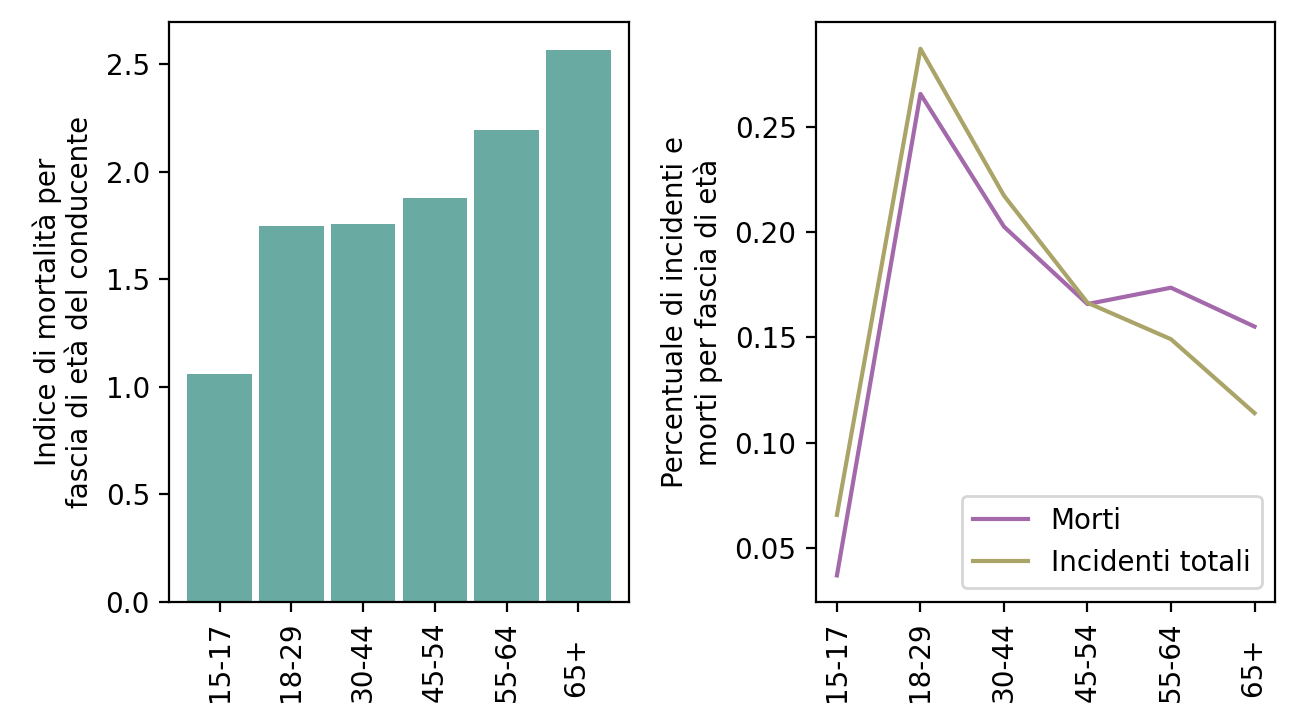
\includegraphics[width=\linewidth]{../src/incidenti/incidenti_senza_coords/mortalita/indice_mort_norm.png}
    \caption{Indice di mortalità degli incidenti, normalizzato per popolazione standard}
    \label{fig:indice-mort-norm}
\end{figure}

Una volta normalizzato per la popolazione standard in Italia, il numero di incidenti per 
fascia di età, nel grafo destro della figura \ref{fig:indice-mort-norm}, mostra che  
si commettono più sinistri nella categoria \columnstyle{18-29 anni}, 
con un calo nei valori successivi.
D'altra parte, l'indice di mortalità non cambia, poichè è realizzato tramite 
un rapporto in cui i fattori sono stati divisi per costanti uguali per ogni fascia.

%\clearpage
\section{Dati ACI}

I dati trovati sul sito di ACI sono inizialmente divisi in due file in 
base al tipo di strada dove l'incidente è avvenuto, 
su autostrade o strade provinciali.
I due gruppi, a loro volta sono rispettivamente divisi in categorie, a seconda 
dell'informazione contenuta, come incidenti con località, incidenti per 
comune, per mese, per giorno della settimana o ora.

\subsection{Incidenti per regione}

Utilizzando i dati ACI, in particolare i file \columnstyle{localizzazione}, è 
possibile dividere gli incidenti per regione e per provincia.
Grazie al dataset geojson di Guglielmo 
Celata\footnote{\url{https://github.com/openpolis/geojson-italy}}, 
è stato possibile realizzare le mappe in figura \ref{fig:incidenti-per-regione}, 
che raffigurano rispettivamente, le regioni con più incidenti 
nelle strade provinciali e nelle autostrade, nell'anno 2018.

Ovviamente il Nord Italia ha il primato per quanto riguarda i sinistri, 
soprattutto nelle regioni di Lombardia, Veneto e Emilia Romagna. 
Spicca poi il Lazio, dove la maggior parte degli incidenti avvengono su autostrade, 
in quanto il volume di questi, in figura \ref{fig:incidenti-per-regione}, 
è nella media nella prima mappa, mentre è il massimo tra tutte le regioni nella seconda.

\todo{allineare}
\begin{figure}
    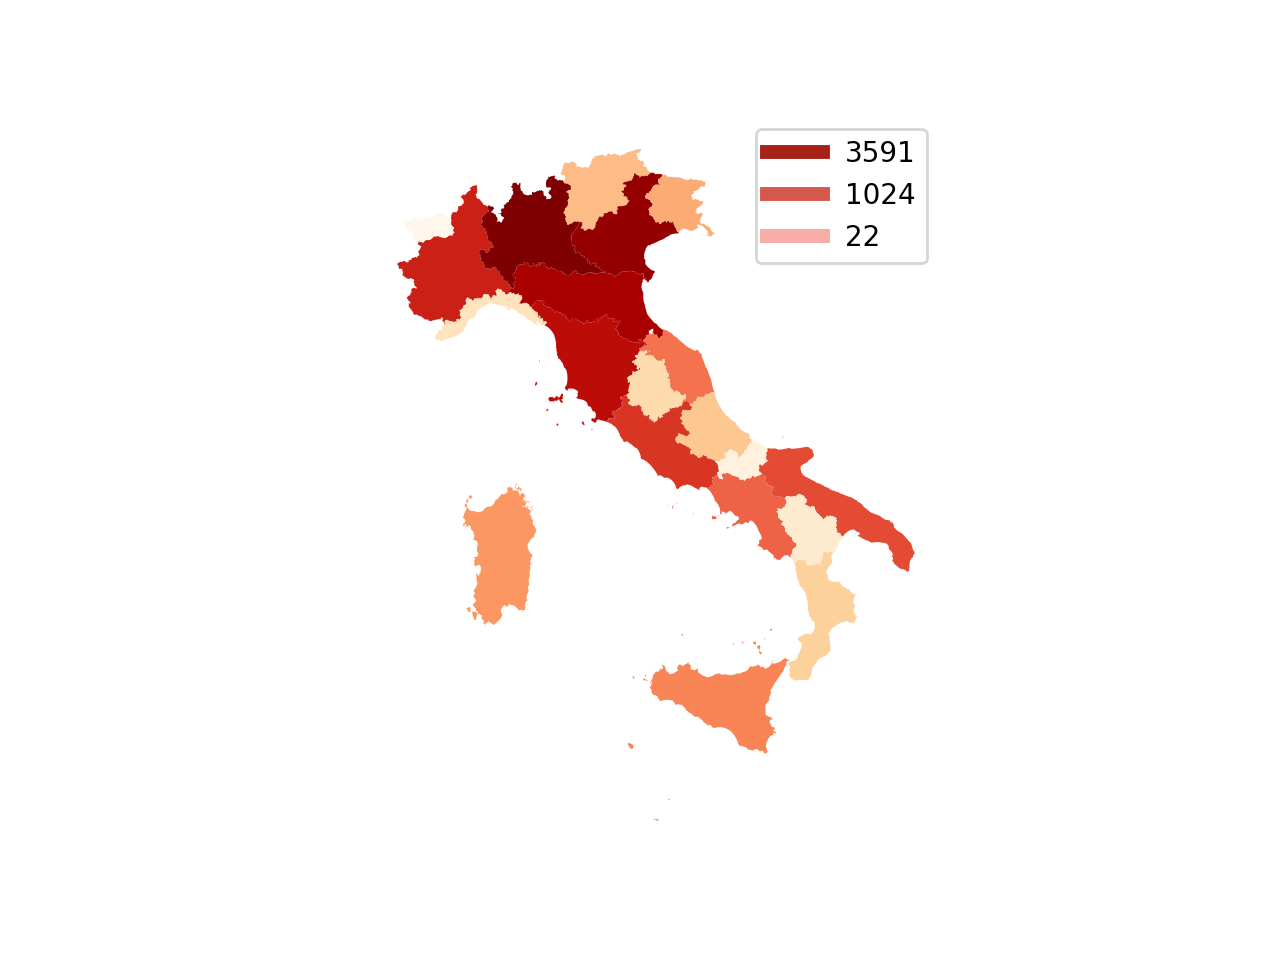
\includegraphics[width=0.5\linewidth]{../src/incidenti/incidenti_aci/mappe_regioni/incidenti_regione.png}
    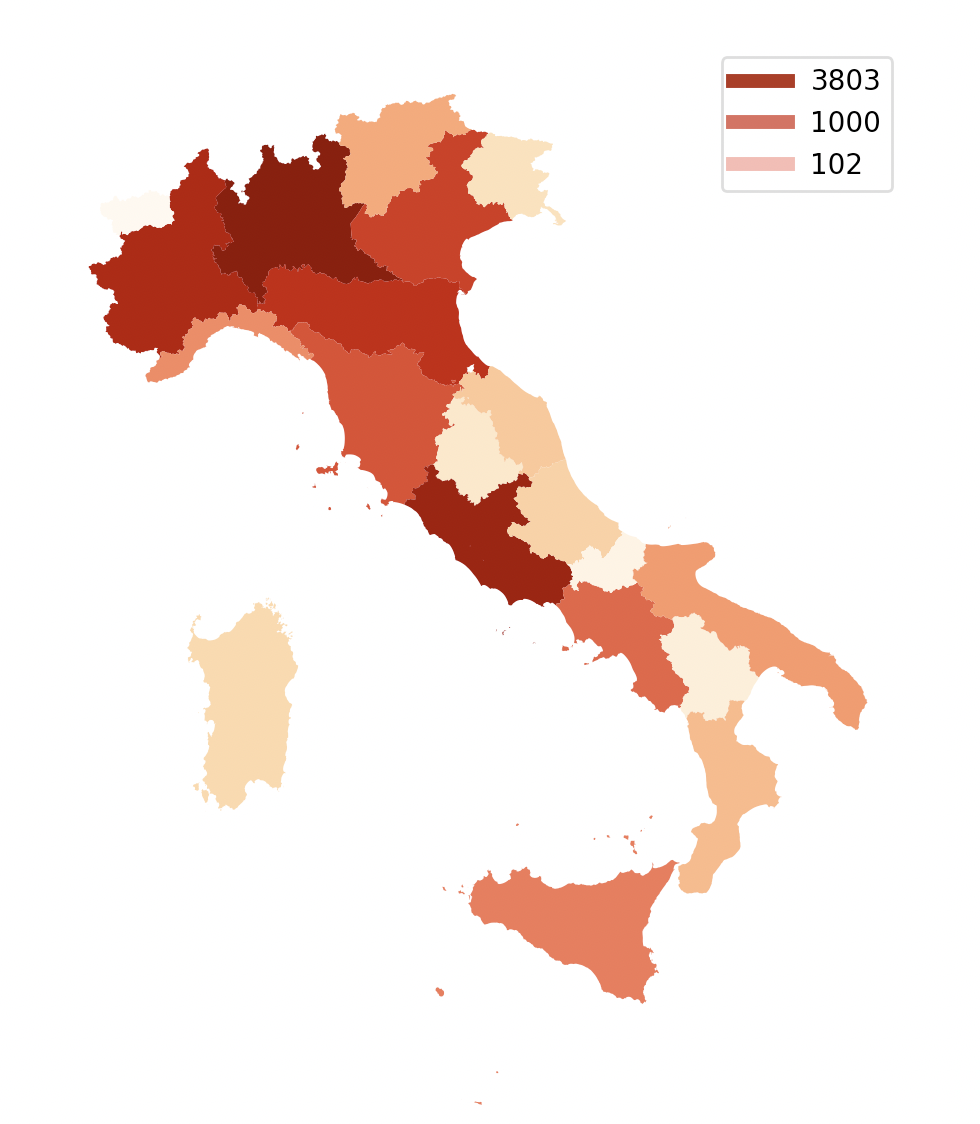
\includegraphics[width=0.5\linewidth]{../src/incidenti/incidenti_aci/mappe_regioni/incidenti_regione_autostrade.png}
    \caption{Incidenti su autostrade e su strade provinciali nel 2018}
    \label{fig:incidenti-per-regione}
\end{figure}

Per quanto riguarda, invece, il numero di incidenti per ogni anno, 
visibile nella heatmap \ref{fig:regione-heatmap} 
si nota che questo non cambia molto di anno in anno, e le regioni con maggiore numero 
di sinistri rimangono sempre Lombardia e Veneto.

Per controllare le tendenze di incremento e decremento di incidenti per regione, 
si è calcolata la deviazione standard per ogni regione\footnote{Deviazione standard: 
misura della distanza dei dati di un campione dalla media\cite{PROB_E_STATISTICA:2}}.
Risulta che la regione con maggiore cambiamento di incidenti di anno in anno 
è il Lazio, con $324$ incidenti l'anno, mentre quella con minore 
variazione è la Valle d'Aosta, con $8$.

\begin{figure}
    \includegraphics[width=\linewidth]{../src/incidenti/incidenti_aci/mappe_regioni/regioni_heatmap.png}
    \caption{Incidenti all'anno per regione su strade provinciali}
    \label{fig:regione-heatmap}
\end{figure}

I grafi precedenti, soprattutto le heatmap regionali, non tengono conto del 
volume del traffico.
Non avendo informazioni riguardanti il traffico in tutta Italia, si sono stimate 
queste informazioni tramite il numero di patentati per regione.
Va sottolineato che una stima eseguita con il numero di patentati per regione, 
non è molto accurata, in quanto molte persone patentate in una regione, possono 
lavorare in altre, e influire in modo errato al conteggio degli incidenti. 

\begin{figure}
    \hfill\includegraphics[width=0.8\linewidth]{../src/incidenti/incidenti_aci/mappe_regioni/incidenti_patenti_italia.png}\hspace*{\fill}
    \caption{Incidenti e patentati per regione}
    \label{fig:incidenti-patentati}
\end{figure}

Se si visualizza il rapporto tra incidenti e patentati per regione 
(figura \ref{fig:incidenti-patentati}), si osserva una chiara distinzione 
tra Nord, Centro e Sud Italia. 
A cosa è dovuta questa ampia disparità?

Nella seguente tabella sono riportate le medie di incidenti annuali per regione, 
e quella di patentati per regione.

\begin{center}
    \def\arraystretch{1.5}%  
    \begin{tabular}{ |c|c|c| } 
    \hline
    Zona & Media Incidenti annuali & Patentati (in Milioni) \\ 
    \hline
    \rowcolor{TableGray}
    Nord    &   2470 &   2.28 \\ 
    Centro  &   2395 &   1.97 \\ 
    \rowcolor{TableGray}
    Sud     &   1145 &   1.57 \\ 
    \hline
    \end{tabular}
\end{center}

Il grafo \ref{fig:incidenti-patentati-bar} è stato suddiviso tra regioni del nord, 
centro e sud per facilitare la lettura, e indica le percentuali di incidenti e 
patentati per la rispettiva regione. 
\'E subito osservabile che, nella maggior parte delle regioni del centro, 
la percentuale di incidenti supera quella di patentati, 
mentre nel Sud Italia accade il fenomeno opposto.

\begin{figure}
    \includegraphics[width=\linewidth]{../src/incidenti/incidenti_aci/mappe_regioni/incidenti_patenti_bar.png}
    \caption{Incidenti e patentati per regione}
    \label{fig:incidenti-patentati-bar}
\end{figure}

La figura \ref{fig:incidenti-patentati-box} permette di capire il motivo della disparità 
tra centro e Sud Italia.
Al sud, il numero di incidenti è molto minore rispetto al centro Italia, mentre, 
sempre le stesse due zone, il numero di patentati non cambia molto. 
\'E ovvio che tenendo il denominatore costante, il numero minore di incidenti al 
sud causa una frazione minore.

\begin{figure}
    \includegraphics[width=\linewidth]{../src/incidenti/incidenti_aci/mappe_regioni/incidenti_patenti_box.png}
    \caption{Incidenti e patentati per Nord, Centro e Sud Italia}
    \label{fig:incidenti-patentati-box}
\end{figure}

Quali potrebbero essere le motivazioni di questa disparità?
Come già accennato in precendenza, una delle motivazioni principali 
deve essere la destinazione lavorativa della popolazione tuttavia, 
come accennato in precedenza, 
la precisione del numero di patenti come fattore utilizzato per la stima 
del traffico non è da considerarsi particolarmente attendibile.

\subsection{Differenze tra mesi estivi e invernali}

Sarebbe interessante controllare se i dati ACI confermino le tendenze trovate tramite 
le informazioni Istat, e vedere se nel Sud Italia, il numero di incidenti crescesca 
come conseguenza delle vacanze estive.

\begin{figure}
    \includegraphics[width=\linewidth]{../src/incidenti/incidenti_aci/mappe_regioni/estate_inverno.png}
    \caption{Incidenti per regione nei mesi estivi e invernali}
    \label{fig:estate-inverno}
\end{figure}

Nella figura \ref{fig:estate-inverno}, sono rappresentati gli incidenti avvenuti 
in mesi invernali ed estivi, divisi per regione. 
In tutte le regioni italiane, il numero di incidenti in estate è maggiore del 
numero di incidenti in inverno. 
La motivazione di ciò è probabilmente il fatto che 
le persone preferiscono muoversi meno nei mesi freddi, rispetto a quelli caldi, 
anche in macchina.

Il comportamento che si stava cercando, cioè più incidenti in estate nel 
Sud Italia, non è visibile. 
D'altra parte, un modo in cui si potrebbe tentare di ricavarlo, è osservare gli 
incidenti sulle autostrade principali in Agosto, su cui si movono i turisti diretti 
nelle località di mare.

Questo tipo di controllo verrà eseguito nei capitoli successivi.

\subsection{Incidenti per provincia}

Utilizzando ancora una volta, i file geojson trovati sul repository github di 
Guglielmo Celata, riguardanti questa volta le province, 
è possibile creare delle heatmap raffiguranti in quali tra queste avvengano più 
incidenti.

Avendo a disposizione dati riguardanti strade provinciali e autostrade, è stato realizzato 
lo stesso calcolo per entrambi i casi.
\todo{allineare}
\begin{figure}
    \includegraphics[width=0.5\linewidth]{../src/provincia/lombardia_autostrade.png}
    \includegraphics[width=0.5\linewidth]{../src/provincia/lombardia_strade_prov.png}
    \caption{Incidenti nelle autostrade e nelle strade provinciali in Lombardia}
    \label{fig:lombardia-strade}
\end{figure}

Nella figura \ref{fig:lombardia-strade} sono mostrati gli incidenti in Lombardia, 
avvenuti rispettivamente nelle autostrade e nelle strade provinciali.
In entrambi i casi, si nota che la provincia di Milano è quella caratterizzata da 
un maggior numero di incidenti. 
D'altra parte, per quanto riguarda le differenze, nelle province di Bergamo e Como, 
i sinistri crescono molto nelle strade provinciali rispetto alle autostrade.

Lo stesso calcolo è stato eseguito per le province del Lazio.
\todo{allineare}
\begin{figure}
    \includegraphics[width=0.5\linewidth]{../src/provincia/lazio_autostrade.png}
    \includegraphics[width=0.5\linewidth]{../src/provincia/lazio_strade_prov.png}
    \caption{Incidenti nelle autostrade e nelle strade provinciali nel Lazio}
    \label{fig:lazio-strade}
\end{figure}

Per quanto riguarda la figura \ref{fig:lazio-strade} raffigurante il Lazio, va 
specificato che il numero di incidenti su autostrade è molto più alto rispetto 
a quello su strade provinciali, 
fenomeno già osservato nella mappa \ref{fig:incidenti-per-regione}.

Inoltre, la provincia di Frosinone ha un numero particolarmente alto di incidenti su 
autostrade, mentre la provincia di Latina, al contrario, ha un maggiore incremento di 
sinistri su strade provinciali.

Non è difficile trovare il motivo di questi numeri, in quanto l'autostrada A01 passa 
attraverso la provincia di Frosinone e non quella di Latina, e conseguentemente provoca 
un'impennata di incidenti nella prima heatmap. 

%\clearpage
\subsection{Le strade pericolose in provincia di Milano}

Approfondendo le informazioni del capitolo precedente, è possibile calcolare quali siano 
le strade più pericolose, per esempio, a Milano. 
Il dataset ACI infatti fornisce il nome delle strade su cui sono avvenuti gli incidenti, 
tuttavia non presenta dati aggiuntivi sulla zona del sinistro, dunque per autostrade molto 
estese, questa misurazione potrebbe presentare errori di vari chilometri. 

Utilizzando il sito Geojson.io\footnote{\url{https://geojson.io/}}, 
è stato possibile tracciare i percorsi delle principali autostrade in prossimità di 
Milano, come le Tangenziali Est e Ovest, la Torino-Trieste e la A1. 
Il risultato è visibile nella figura \ref{fig:line-incidenti-milano}.

\begin{figure}
    \includegraphics[width=\linewidth]{../src/incidenti/incidenti_aci/autostrade/incidenti_line_chart.png}
    \caption{Autostrade con più incidenti nel 2018}
    \label{fig:line-incidenti-milano}
\end{figure}

In particolare, dalla mappa \ref{fig:line-incidenti-milano}, si deduce che le 
Tangenziali Ovest e Est, e l'autostrada Torino-Trieste, sono i tratti di 
strada con maggior numero di incidenti, con più di $150$ sinistri all'anno.

Infine, se si avesse a disposizione la posizione precisa degli incidenti, 
sarebbe possibile anche dividere queste tratte, in sezioni più piccole, 
e controllare se esistano zone che alzano il volume di incidenti, poichè 
particolarmemte pericolose.

%\clearpage
\subsection{Esiste correlazione tra incidenti e feriti?}

Utilizzando i dataset ACI a disposizione, è possibile stabilire l'esistenza di 
correlazione tra morti e incidenti, o tra morti e feriti?
Ovviamente ci si aspetta che la risposta abbia un esito positivo, poichè 
i campioni di feriti e morti sono strettamente collegati al numero di sinistri.

L'indice di correlazione utilizzato è il coefficiente di Pearson, 
calcolato tramite la formula: 

\begin{center}
    $\rho_{X, Y} = \displaystyle \frac{cov(X, Y)}{\sigma_X \sigma_Y}$
\end{center}

\begin{center}
    con: $\rho_{X, Y} \rightarrow [-1, 1]$
\end{center}

dove X e Y sono i due campioni tra cui si vuole calcolare la correlazione, 
\methodstyle{cov()} restituisce la covarianza, e $\sigma_X$ è la deviazione standard del 
campione X \cite{PROB_E_STATISTICA:3}. 

Una volta divisi i dati, è possibile calcolare l'indice tramite il metodo 
\methodstyle{corr()}, i risultati sono riportati nella seguente tabella.

Il valore restituito dal metodo \methodstyle{corr()} è contenuto tra $-1$ e $1$ dove, 
se il numero si avvicina a uno, è possibile dire che tra i due campioni esista correlazione 
lineare, mentre la vicinanza all'altro estremo indica la presenza di correlazione inversa.

\begin{center}
    \def\arraystretch{1.5}%  
    \begin{tabular}{ |c|c|c| } 
    \hline
    Incidenti & Incidenti & Feriti \\ 
    Feriti & Morti & Morti \\ 
    \hline
    0.9836 & 0.3385 & 0.3355 \\ 
    \hline
    \end{tabular}
\end{center}

\begin{figure}
    \includegraphics[width=\linewidth]{../src/incidenti/incidenti_aci/provincia/corr_incidenti.png}
    \caption{Correlazione tra numero di feriti e incidenti nelle venti province con maggior numero di sinistri}
    \label{fig:corr-incidenti-feriti}
\end{figure}

Tracciando il grafo \ref{fig:corr-incidenti-feriti}, contenente i primi trenta valori 
del dataset ACI, è chiaramente visibile la correlazione tra 
numero di incidenti e di feriti, in quanto nella maggior parte dei casi, 
all'aumentare dei primi il volume dei secondi cresce allo stesso modo.

L'unico dubbio che possa sorgere è che il numero di infortunati sia maggiore di quello 
di incidenti, tuttavia controllando il dataset, ogni 
riga contiene più feriti rispetto a sinistri.
\'E possibile che il dataset contenga solo incidenti con almeno un ferito, 
e quindi ignori tutti i sinistri non particolarmente significativi.
D'altra parte, tenendo conto che si sono utilizzati dati raccolti lungo 
le autostrade, è possibile che la maggior parte degli scontri comporti 
un alto numero di feriti. 
Nella tabella sottostante è raffigurato un estratto del dataset ACI, 
di cui si sono prese in considerazione le colonne principali, più 
rilevanti per questo calcolo. 

\begin{center}
    \def\arraystretch{1.5}%  
    \begin{tabular}{ |c|c|c|c| } 
    \hline
    Provincia & Comune & Incidenti & Feriti \\ 
    \hline
    \rowcolor{TableGray}
    Torino & Brandizzo & 5 & 10\\
    Torino & Chivasso & 12 & 18\\
    \rowcolor{TableGray}
    Torino & Rondissone & 6 & 12\\
    Torino & Settimo Torinese & 25 & 40\\
    \hline
    \end{tabular}
\end{center}

Il coefficiente di Pearson, per quanto riguarda i campi \columnstyle{Incidenti} 
e \columnstyle{Feriti}, 
è molto vicino a uno, quindi i due campioni sono strettamente correlati.
Nonostante, in generale, correlazione non implichi causa o effetto, cioè, non 
è detto che due fattori correlati si influenzino in alcun modo, in questo caso è 
difficile pensare che il numero di incidenti non sia il motivo dell'aumentare o diminuire 
dei feriti.
I coefficienti riguardanti i morti sono molto meno vicini a uno, probabilmente 
per il minor numero di sinistri mortali, che rende il campione più ristretto.

\subsection{Le autostrade più pericolose}

Il dataset ACI raggruppa in un solo dataset sia le autostrade che le strade statali, 
esitono differenze sostanziali tra le due categorie?
La maggiore capienza di veicoli lungo le autostrade porta queste a occupare i primi 
posti per quanto riguarda le strade con più sinistri?
\'E possibile utilizzare i file con incidenti 
localizzati\footnote{Per localizzati si intende che è stato riportato nel dataset 
il nome della strada in cui è avvenuto il sinistro}, 
per tentare di rispondere a queste domande.

\begin{figure}
    \includegraphics[width=\linewidth]{../src/incidenti/incidenti_aci/autostrade/autostrade.png}
    \caption{Autostrade e strade statali con più incidenti nel 2018}
    \label{fig:incidenti-autostrade}
\end{figure}

Nella figura \ref{fig:incidenti-autostrade} sono  raffigurate le strade con 
maggiore numero di incidenti nel 2018. 
Non è una sorpresa che le prime posizioni della lista coincidano 
anche con le strade più trafficate, come l'Autostrada del Sole e l'Adriatica, 
tuttavia sono anche presenti, due strade statali, la SS1 e la SS16. 

La motivazione dell'alto numero di incidenti su queste direttrici, potrebbe essere 
la lunghezza di queste. Infatti entrambe sono strade che corrono lungo tutta la 
costa Italiana da nord a sud e, nella maggior parte della loro estensione, 
hanno solamente due corsie.

L'avere i sensi di marcia separati, e delle corsie designate al sorpasso, nel caso 
delle autostrade non può che essere un fattore che influenza negativamente 
il numero degli incidenti. 
D'altra parte, l'essere costretti a sorpassare sulla corsia adibita al senso di 
marcia opposto, nel caso della SS1 e SS16, può portare a un aumento dei 
sinistri.
Va sottolineato che quelle riportate sono solamente ipotesi, e che servirebbero 
dati più precisi per capire se esistano tratti particolarmente 
pericolose lungo queste strade.

\subsection{Tratte pericolose lungo le principali strade statali}

Un modo per aumentare la precisione dei dati a disposizione, potrebbe essere il 
dividere gli incidenti sulle strade statali, in base alla provincia in cui sono avvenuti.

Nonostante il procedimento sia stato eseguito solo per le strade statali, gli stessi dati 
sono presenti anche per le autostrade e le strade provinciali, e un'analisi più 
approfondita potrebbe includere queste informazioni.
\todo{allineare}
\begin{figure}
    \includegraphics[width=0.5\linewidth]{../src/incidenti/incidenti_aci/statali/ss01_tratti.png}
    \includegraphics[width=0.5\linewidth]{../src/incidenti/incidenti_aci/statali/ss16_tratti.png}
    \caption{Incidenti su SS1 e SS16, divisi per provincia in cui questi sono avvenuti}
    \label{fig:incidenti-strade-statali}
\end{figure}

Nel grafo sinistro della figura \ref{fig:incidenti-strade-statali}, contiene il numero di 
incidenti, oltre a quello di persone ferite, avvenuti in ogni provincia attraversata dalla SS1. 
La provincia in cui avvengono più sinistri è quella di Savona, mentre le grandi città come 
Roma e Livorno hanno valori nella media o poco superiori.

Lo stesso grafo, realizzato per la SS16, è rappresentato nella figura destra dell'immagine 
\ref{fig:incidenti-strade-statali}. 
In questo caso, il picco di scontri avviene nella provincia 
di Bari, con quasi $200$ incidenti e $400$ feriti nel 2018. 

Una provincia che salta all'occhio invece, per dei valori bassi è quella di Pescara. 
Dopo aver eseguito il codice sottostante, tuttavia, si è osservato che tutte le righe 
del dataset per questa zona riportano valori uguali a zero, eccetto una. 

\begin{code}
data = pd.read_csv("dataset/incidenti/aci/autostrade/localizzazione_2018.csv")
ss16 = data[data['CODICE'] == 'SS01601']

pescara = ss16[ss16['PROVINCIA'] == 'Pescara'][['INC', 'FER']]
\end{code}

A prima osservazione questo risulato potrebbe essere considerato un errore nei dati. 
Tuttavia, considerando che l'estensione della SS16 in questa provincia non 
è particolarmente ampia, è plausibile che durante l'anno sia avvenuto un solo incidente. 
A supportare questa teoria, nella figura \ref{fig:ss16-pescara} si osserva come 
questa direttrice, all'ingresso in città, diventi strada urbana e, molto probabilmente, 
sia registrata con un altro nome.

\begin{figure}
    \includegraphics[width=0.5\linewidth]{img/pescara_ss16.png}
    \caption{La SS16 nella provincia di Pescara. All'ingresso in città questa strada cambia nome in SS714}
    \label{fig:ss16-pescara}
\end{figure}

Da un'analisi di questo tipo, non è facile trarre conclusioni approfondite, in quanto la 
zona in cui può essere avvenuto l'incidente è particolarmente ampia, e il numero maggiore di 
sinistri in un luogo potrebbe essere semplicemente dovuto alla maggiore estensione della 
strada in quella provincia. 
Inoltre, a eccezione di alcune province, come Bari, Savona, Viterbo e Massa-Carrara, 
la maggior parte degli scontri è più o meno omogeneamente distributo lungo tutta 
l'estensione delle direttrici. 

Se si avesse a disposizione la lunghezza delle due strade in questione, 
o anche il flusso di automobili nelle province attraversate, 
si potrebbe controllare quanto questo fattore influisca sul volume di incidenti. 

\subsection{Le autostrade più utilizzate in estate cambiano a seconda dell'anno?}

Tornando a concentrarsi sulle autostrade, sarebbe interessante sapere se quelle 
con più incidenti cambino al cambiare dell'anno.
Una motivazione di questo fenomento potrebbe essere, il cambiamento 
delle mode riguadanti le località di vacanza.
Per esempio, nel 2018, le mete preferite sono state Puglia e 
Toscana\cite{INFOGRAFICA_ISTAT:1}, mentre nel 2019, oltre alla Puglia, 
una percentuale sostanziale di turisti si è recata in 
Emilia Romagna e Liguria\cite{REPORT_ISTAT_2019:1}.

Avendo a disposizione i dati di tutte le annate, dal 2010 al 2018, 
è possibile controllare se esistano anni con un volume di 
incidenti in Agosto particolarmente alto.

\begin{figure}
    \includegraphics[width=\linewidth]{../src/incidenti/incidenti_aci/agosto/vacanze_autostrade.png}
    \caption{Incidenti in strade per anno nel mese di Agosto}
    \label{fig:autostrade-anno}
\end{figure}

Controllando le prime cinque strade per incidentalità ogni anno, 
raffigurate nel grafo \ref{fig:autostrade-anno}, si ottiene un'immagine 
abbastanza consistente, in quanto le direttrici in testa alla classifica sono 
sempre le stesse.

La strada statale Adriatica è sempre in prima posizione, con una media di $171.5$ 
sinistri nel mese di Agosto.
Le posizioni successive invece cambiano a seconda dell'anno, in particolare però, 
nell'autostrada A4 (Torino-Trieste) il numero di incidenti è progressivamente cresciuto, 
evento possibilmente dovuto all'aumento di popolarita delle vacanze 
in montagna anche nel periodo estivo.

Facendo utilizzo del dataset Istat riguardante il turismo in Italia, e in 
particolare sfruttando due indicatori, Tasso di 
Turisticità\footnote{Tasso di Turisticità: indica il numero di turisti 
presenti ogni 100.000 abitanti\cite{ONTIT:1}} 
e turismo in mesi non estivi, è stato possibile realizzare il grafo \ref{fig:turismo}, 
contenente questi indici, nel periodo a partire dall'anno 1995 fino al 2018.

\begin{figure}
    \includegraphics[width=\linewidth]{../src/turismo/turismo.png}
    \caption{Turismo nelle principali località estive e invernali}
    \label{fig:turismo}
\end{figure}

Nel grafo \ref{fig:turismo} sono state incluse alcune regioni con località popolari 
per le vacanze estive, come Sardegna, Sicilia e Liguria, e regioni principalmente 
di montagna, come Trentino e Valle d'Aosta. 
La Lombardia, infine, è stata aggiunta per assicurarsi che il trend delle due regioni 
di montagna non fosse comune a tutte le regioni del Nord Italia.

Ciò che si può concludere, oltre al fatto che le zone di montagna abbiano 
un tasso di turisticità particolarmente alto, probabilmente per il numero 
ristretto di abitanti, 
è che, a partire dal 2015, è presente una crescita nel volume di turisti nelle località 
del Nord Italia a eccezione della Lombardia, che non è visibile nelle 
destinazioni di mare.

In particolare, rispetto al 2015, in Trentino nel 2018 si ha un incremento 
di turisti percentuale del $11.9$\%, mentre eseguendo lo stesso calcolo con la 
media\footnote{Calcolata sull'insieme di anni disponibili, quindi 
a partire dal 1995 fino al 2018} l'aumento è del $14.7$\%.

In Valle d'Aosta, allo stesso modo, l'incremento di turisti nel 2018 
rispetto al 2015 è del $13$\%, mentre rispetto alla media annuale 
è del $7.6$\%.

Va sottolineato infine, che non è possibile dire con sicurezza che 
la crescita in popolarità delle zone di montagna sia alla causa dell'aumento 
di incidenti sull'autostrada Torino-Trieste. 
Infatti, su quest'ultima, il numero di sinistri rimane relativamente costante, 
con $99$ scontri nel 2011, e $97$ nel 2018.

\subsection{L'incidentalità su autostrade dipende dai mesi dell'anno?}

Un'altra questione, di cui ci si è occupati tramite dati Istat in precedenza, è 
quella dei mesi con maggiore incidentalità.
Il dataset ACI permette di individuare gli stessi cambiamenti di tendenza trovati nei 
capitoli precedenti, in più però permette di dividere i sinistri in base alla strada.

In particolare, nell'analisi precedente si era individuato un decremento di incidenti 
nei mesi estivi nella zona di Milano, e il comportamento opposto nelle province di 
Rimini e Aosta.

\begin{figure}
    \includegraphics[width=\linewidth]{../src/incidenti/incidenti_aci/autostrade/mesi_autostrade.png}
    \caption{Incidenti per mese nel 2018}
    \label{fig:incidenti-per-mese}
\end{figure}

La heatmap \ref{fig:incidenti-per-mese} mostra che su alcune autostrade, come il 
Grande Raccordo Anulare a Roma, il numero di incidenti diminuisce durante i mesi 
estivi.
D'altra parte, la tendenza opposta avviene, per esempio, sulla A1 e la A4, 
con picchi di sinistri in Giugno e Luglio per, come precendentemente spiegato, 
l'aumento di traffico dovuto alle partenze per le vacanze.
Sull'Adriatica e sull'Aurelia, infine, prevalgono scontri 
in Luglio e Agosto e in generale nei mesi estivi.

\begin{figure}
    \includegraphics[width=\linewidth]{../src/incidenti/incidenti_aci/autostrade/adriatica_roma.png}
    \caption{Incidenti sull'Adriatica e sul Grande Raccordo Anulare a Roma nel 2018}
    \label{fig:adriatica-roma}
\end{figure}

Isolando gli incidenti avvenuti sul Grande Raccordo Anulare a Roma, e quelli avvenuti 
sull'Adriatica, raffigurati nel grafo \ref{fig:adriatica-roma}, si osserva, 
nel primo caso, un numero di sinistri per mese molto omogeneo, a eccezione del 
mese di Agosto, quando avviene un calo del $46$\% rispetto alla media mensile. 
D'altra parte, nel caso dell'Adriatica, è visibile una campana con apice nei 
mesi di Luglio e Agosto, comportamento opposto rispetto a quello nell'autostrada 
romana.

Come ultimo quesito, bisognerebbe domandarsi se ha senso dire che il mese dell'anno 
influenzi l'incidentalità. 

Di certo il questo indicatore sembra essere un buon stimatore 
per i numero di sinistri.
Tuttavia va ricordato che sono tutti i fattori 
nascosti in questa indagine, che variano mensilmente, a influenzare l'esito. 

%\clearpage%
\subsection{In quali orari avvengono incidenti sulle autostrade?}

Rimanendo sull'argomento delle analisi già eseguite per dati Istat, 
si potrebbe replicare, con i dati ACI, quella riguardante gli orari di incidenti. 
Avendo a disposizione il nome della strada, è possibile selezionare delle zone precise 
di strade su cui avvengono molti sinistri, come la SS1 e SS16.

\begin{figure}
    \includegraphics[width=\linewidth]{../src/incidenti/incidenti_aci/orari/orari.png}
    \caption{Incidenti all'anno per orario su strade e località italiane diverse}
    \label{fig:orari-strade-aci}
\end{figure}

Nella figura \ref{fig:orari-strade-aci} sono raffigurati gli incidenti avvenuti 
nel 2018, divisi per orario, sulla SS16 Adriatica in provincia di Bari, sulla SS1 
in provincia di Genova, e infine sul Grande Raccordo Anulare a Roma.

Le tendenze visibili nei tre grafi sono molto simili tra loro. 
A Roma, dove si ha maggiore 
volume di incidenti, si osservano picchi nelle fasce orarie delle 
7:00-9:00 e delle 17:00-19:00, già evidenziate nei capitoli precedenti sull'argomento. 

Prendendo in considerazione invece, la città di Milano, si potrebbero ricavare 
informazioni interessanti su quali sono le strade più utilizzate per 
andare e tornare dai luoghi di lavoro.

\begin{figure}
    \includegraphics[width=\linewidth]{../src/incidenti/incidenti_aci/orari/tangenziali_autostrade.png}
    \caption{Incidenti nelle principali autostrade di Milano per orario}
    \label{fig:tangenziali-autostrade}
\end{figure}

Il grafo \ref{fig:tangenziali-autostrade} conferma, per alcune autostrade, 
l'esistenza di picchi di incidenti durante orari di punta. 
In particolare è molto visibile per la A4 Torino-Trieste, 
per la Tangenziale Ovest e per la Tangenziale Est.

\'E possibile ipotizzare che queste siano le strade più utilizzate per 
andare a lavoro? 
Certamente la maggior parte dei residenti a Milano non utilizzerà strade registrate 
nell'ultimo grafo, poichè essendo già a Milano, utilizzaranno le direttrici urbane. 
Tuttavia, per quanto riguarda i pendolari, è molto probabile che, quelli provenienti 
da Varese, Busto Arsizio o Novara per esempio, utilizzino la Tangenziale Ovest, 
e dunque siano registrati nei conteggi. 

Questa stima, di certo non permette di affermare con sicurezza 
che la maggior parte dei pendolari utilizzano le strade prese in considerazione 
nei grafi.
Tuttavia, gli incidenti durante le ore di punta sulle autostrade A4 e sulle 
Tangenziali sono particolarmente alti e, avendo a disposizione dati più 
precisi, per esempio sui pendolari, sarebbe possibile realizzare analisi 
più approfondite.

%\clearpage
\subsection{Quali autostrade sono utilizzate di più per viaggiare in Agosto?}

Nel capitolo precedente si è tentato di trovare quali strade siano maggiormente 
utilizzate per recarsi a lavoro a Milano. 
Sarebbe interessante realizzare un calcolo simile, per quanto riguarda le autostrade 
più percorse per spostarsi in località di vacanza. 

Non è un segreto che, nel mese di Agosto, si abbia il maggior numero di 
partenze per le vacanze e, in genere, per quanto riguarda i viaggi 
in macchina, la tendenza è quella di spostarsi verso sud, 
per raggiungere le zone balneari.
Spesso, ciò comporta bollini rossi e neri per le autostrade. 

\begin{figure}
    \includegraphics[width=\linewidth]{../src/incidenti/incidenti_aci/agosto/autostrade_anno_agosto.png}
    \caption{Autostrade con più incidenti per anno, in Agosto}
    \label{fig:autostrade-anno-agosto}
\end{figure}

Il grafo \ref{fig:autostrade-anno-agosto} contiene informazioni riguardanti 
in quali autostrade sono avvenuti più incidenti nel mese di Agosto del rispettivo anno. 
In questo grafo, si è tentato un approccio diverso rispetto a quello del capitolo precedente, 
elencando le autostrade più trafficate per anno e numero di sinistri, invece di usare una 
heatmap, come nella figura \ref{fig:autostrade-anno}.

I colori delle barre, nel grafico \ref{fig:autostrade-anno-agosto}, sono stati aggiunti per 
facilitare la lettura delle strade, infatti colori diversi corrispondono a direttrici diverse. 

In particolare spiccano la SS16 Adriatica e SS1 Aurelia che, come già 
detto in precedenza, essendo strade statali molto lunghe e con corsie di marcia 
non separate, devono essere più pericolose rispetto alle autostrade.
Per non parlare del fatto che entrambe le strade passano attraverso un 
alto numero di centri abitati.

\'E anche curioso che le uniche autostrade presenti nel grafo siano la A1 e la A14, 
solamente in occasione dell'estate 2011. 
La motivazione di ciò potrebbe essere, che le due strade statali, oltre a essere usate per 
recarsi nella località marittima, siano poi sfruttate anche durante la vacanza per 
raggiungere zone vicine, mentre è molto più raro che, durante le ferie, una famiglia 
si rechi in spiaggia viaggiando su un'autostrada.

\chapter{Dati su Meteo}

\section{Meteo a Milano}

\subsection{Correlazione tra fattori atmosferici e incidentalità}

L'idea di ipotizzare che esista correlazione tra le condizioni meteo e il numero 
di incidenti, può non sembrare improponibile, in fondo a nessuno piace guidare 
durante una nevicata.
Tuttavia, le informazioni necessarie per ottenere una stima della correlazione 
dei due fattori sono, o fuori dalla portata dei dati liberi, o inesistenti. 

Un esempio di questi dati, potrebbe essere il sapere giorno e ora 
dell'incidente, e allo stesso modo anche le zone in cui si sono verificati certi 
fenomeni atmosferici, come la caduta di neve. 
Entrambi questi dati non sono disponibili tramite dataset aperti, e probabilmente, 
anche con questi non sarebbe possibile dare una buona stima della correlazione 
tra i due fattori.

\'E comunque interessante mostrare come, la correlazione tra due campioni possa essere 
estremamente alta, anche se questi ultimi sono completamente scollegati.
\todo{allineare}
\begin{figure}
    \includegraphics[width=0.5\linewidth]{../src/meteo/temp_incidenti_2011.png}
    \includegraphics[width=0.5\linewidth]{../src/meteo/temp_incidenti_2013.png}
    \caption{Incidenti, temperature e umidità medi per mese nel 2011 e nel 2013}
    \label{fig:incidenti-temp}
\end{figure}

La figura \ref{fig:incidenti-temp} mostra, partendo dall'alto, il numero di incidenti 
avvenuti per mese, la temperatura media per mese, e infine l'umidità media.
Sono riportati i due anni con, rispettivamente la maggiore e la minore correlazione tra 
incidenti e fattori atmosferici.

Non è stato possibile eseguire la stessa operazione con dati più recenti, per mancanza del 
campo \columnstyle{mese}, convertito in \columnstyle{trimestre} a partire dal 2014.
I risultati sono riportati nella tabella sottostante: 

\begin{center}
    \def\arraystretch{1.5}%  
    \begin{tabular}{ |c|c|c|c| } 
    \hline
    Anno & Temperatura & Velocità del Vento & Umidità \\ 
    \hline
    \rowcolor{TableGray}
    2010 & 0.768 & 0.585 & -0.626 \\
    2011 & 0.900 & 0.626 & -0.730 \\
    \rowcolor{TableGray}
    2012 & 0.732 & 0.501 & -0.609 \\
    2013 & 0.658 & 0.465 & -0.516 \\
    \hline
    \end{tabular}
\end{center}

Per le annate a disposizione, i dati sono consistenti tra loro, e indicano la presenza di 
correlazione lineare tra temperature e incidenti, mentre si ha correlazione inversa per quanto 
riguarda l'umidità.

Ciò non significa che, per esempio nel 2011, sia stata l'alta temperatura a provocare 
tutti gli incidenti, anzi, è molto più probabile che il fattore con maggiore 
influenza sia proprio il mese, e non la temperatura o l'umidità.

Infatti, se si osserva che tipo di informazioni si sta utilizzando 
queste stime, il dataset sulle condizioni meteo è molto impreciso, in quanto potrebbero 
esserci differenze di diversi gradi, in zone lontane di Milano.
Allo stesso modo, anche i dati sugli incidenti non sono particolarmente precisi, 
visto che indicano solo il nome dell'autostrada in cui è avvenuto 
il sinistro, e la posizione effettiva potrebbe essere a chilometri di distanza da dove 
si è calcolata l'informazione sul meteo.

Dal punto di vista, invece, della velocità del vento, sarebbe possibile eseguire 
un'analisi più approfondita, in quanto un valore dell'indice di correlazione uguale 
a $0.5$ non è particolarmente alto.
Si potrebbe, per esempio, controllare se esista una qualche differenza tra gli 
incidenti su moto rispetto all'auto. 
Oppure, avendo a disposizione la velocità del vento in una precisa zona, controllare 
il volume di sinistri all'uscita delle gallerie, zone molto pericolose 
in presenza di vento forte.

Infine, osservando le misurazioni sull'umidità, è possibile che in questo caso sia presente 
un rapporto di causa e effetto, in quanto spesso, un valore alto di questo fattore 
coincide con pioggia e temporali, che a loro volta rendono più difficoltosa la guida.


\chapter{Conclusioni}
\todo{atrent: ricapitolare gli scopi}

Per concludere, sarebbe opportuno riportare quali siano state le maggiori difficoltà 
incontrate durante l'analisi di dati liberi appena realizzata.

Uno dei problemi riscontrati, soprattutto per quanto riguarda il confermare la 
validità dei risultati calcolati, è stata la mancanza di dataset in ambiti come 
il traffico e il fondo stradale. 
Per ovviare a questa difficoltà si è spesso dovuto ricorrere a stime, 
come il numero di accessi in area C. 
L'assenza di informazioni ha giocato un ruolo anche nelle analisi riguardanti gli incroci, 
in quanto non si sono trovati riferimenti al numero di questi in alcun sito di open data.


In secondo luogo, alcuni dataset non sono completi, o hanno sezioni temporali mancanti,
estese anche svariati mesi. 
\'E il caso delle informazioni sugli accessi all'area C di Milano dove, 
per il 2013 non è presente il mese di Dicembre.

Rimanendo sull'argomento, lo stesso dataset, a partire dal 2017, è disponibile 
solamente diviso in dodici file su base mensile.
Questo, in passato, era un comportamento ricorrente, in 
quanto molte piattaforme, come quella del Ministero dei 
Trasporti\footnote{\url{http://dati.mit.gov.it/catalog/dataset}}, 
misuravano le condivisioni di open data delle amministrazioni 
sulla base del numero di file pubblicati.
Era quindi più proficuo pubblicare dati separati, rispetto a tutte le informazioni in 
un unico dataset.
\todo{atrent: a me pareva di averlo segnalato, non c'è da nessuna parte una 
introduzione all'opendata, in cui si potrebbe dire cosa sono, come vengono 
classificati (Berners-Lee e Davies) e quali siano i processi di pubblicazione}

Ovviamente questa operazione rende non solo la raccolta delle informazioni più complessa, 
ma anche l'associazione di dati, che magari sono presenti in un file e non in un altro. 
Il sito Global Open Data Index, che offre un punteggio in base a quanti dati ogni paese 
ha condiviso in formato libero, nelle metodologie di calcolo di questo, scrive: 

\begin{center}
    \quotestyle{\dots we expect that national governments also provide aggregation 
    of that data from 
    sub governments so as to ensure users have an easy way to access use the data 
    (the best solution is one consolidated dataset but at a minimum could consist of a 
    single point of access to all data subsets).}\cite{OPENDATAINDEX:1}
\end{center}

\begin{center}
    \quotestyle{\dots Ci si aspetta che i governi nazionali provvedano per 
    l'aggregazione dei dati provenienti dalle 'regioni', per garantire agli utenti 
    un punto di accesso 
    alle informazioni (la soluzione migliore sarebbe l'avere un dataset unico, ma è sufficiente 
    avere un solo punto di accesso a tutti i sottoinsiemi di dati).}
\end{center}

\todo{atrent: riesci a trovare qualche articolo che ne parla? 
te lo avevo detto io ma sarebbe carino trovare qualcuno che lo abbia detto pubblicamente, 
anche solo su web, era una cosa tipo "valutazione delle PA nell'opendata"}

\todo{lelepado: questa come fonte può andare? non ho trovato articoli...}

\todo{\url{https://www.europeandataportal.eu/sites/default/files/open_data_maturity_report_2019.pdf}}
\todo{\url{https://www.forumpa.it/open-government/open-data/open-data-maturity-report-2019-linsostenibile-leggerezza-dellimpegno-italiano/}}
\todo{\url{https://www.europeandataportal.eu/sites/default/files/country-factsheet_italy_2019.pdf}}
\todo{\url{https://www.agid.gov.it/sites/default/files/repository_files/documentazione/strat_crescita_digit_3marzo_0.pdf}}

\skipline
Infine, un problema sorto con frequenza è stato la mancanza di descrizioni sul 
significato dei campi di una tabella. 
\todo{atrent: appunto, classificazione ;)}
Un esempio di ciò, in figura \ref{fig:scheda-metadati}, sono i dati provenienti dal 
geoportale del comune di Milano, 
in particolare i dataset riguardanti la rete dei trasporti e il manto stradale.
In molti casi, si è dovuto ipotizzare il significato delle colonne delle tabelle, 
e di conseguenza si è stati costretti a scartare queste informazioni. 

\begin{figure}
    \hfill\includegraphics[width=0.7\linewidth]{img/scheda_metadati_geoportale.png}\hspace*{\fill}
    \caption{Pagina dei metadati del dataset riguardante il manto stradale (Geoportale Milano)}
    \label{fig:scheda-metadati}
\end{figure}
\todo{atrent: metterei almeno uno screenshot, sicuro che non c'è 
descrizione campi?}

Analogamente, molti dataset non aderiscono ad 
alcuno standard, per quanto riguarda la nomenclatura delle colonne.
Nelle tabelle provenienti dal sito Istat, per esempio, nel 2011, hanno un campo denominato 
\columnstyle{intersezione\_o\_non\_interse1}, mentre nel 2018, la stessa informazione ha 
nome \columnstyle{intersezione\_o\_non\_interse3}. 

A cambiare non sono soltanto i nomi delle colonne negli anni, ma in alcuni casi, 
come quello esplorato in precedenza, è usato un solo \quotestyle{underscore} a 
simboleggiare uno spazio, mentre nel campo \columnstyle{veicolo\_\_a\_\_\_et\_\_conducente} 
ne sono usati due o anche tre.

Rimanendo in tema, lo stesso dataset Istat ha colonne con differenze di anno in anno, 
come \columnstyle{mese}, che è presente fino al 2013, e successivamente viene 
sostituito dal campo \columnstyle{trimestre}. 
In questo caso, non solo è presente un cambio di nomenclatura, ma il dato in sè è 
anche reso più vago.

\chapter{Utilizzo del Codice}

Tutti gli script utilizzati per questo lavoro sono reperibili a questa pagina 
github: \url{https://github.com/lelepado01/Tirocinio}.

Il repository è diviso in tre cartelle principali, \filenamestyle{dataset}, \filenamestyle{src} 
e \filenamestyle{tesi}. La prima contiene tutti i file di informazioni utilizzati, divisi per 
argomento, e alcuni documenti di testo riguardanti le stime realizzate, come la percentuale di 
conducenti maschio e femmina.

La cartella \columnstyle{tesi} contiene la maggior parte delle immagini utilizzate 
nella relazione\footnote{Ci si riferisce alle immagini realizzate tramite screenshot 
da Google Maps e altri siti, non ai grafi.} 
e il codice sorgente \LaTeX del pdf.

Infine, nella directory \filenamestyle{src} è contenuto il codice sorgente utilizzato per realizzare 
i grafi, le mappe e le stime, diviso per argomento. 
Ogni grafo è associato allo script python che ne permette la creazione, registrato con 
lo stesso nome, e estensione \filenamestyle{.py}. 
Quindi se in una cartella fosse presente l'immagine \filenamestyle{esempio.png}, lo script con 
cui questa è stata creata avrà nome \filenamestyle{esempio.py}.

Invece, se si volessero trovare le informazioni sul grafo raffigurante 
l'incremento di incidenti 
dal 2010 al 2018, i dataset utilizzati si troverebbero nella directory:

\skipline
\indent\filenamestyle{dataset/incidenti/incidenti\_istat}

\skipline
\noindent Mentre il codice sorgente e le immagini sarebbero situate al percorso:

\skipline
\indent\filenamestyle{src/incidenti/incidenti\_senza\_coords/anno}

\skipline
Infine, in modo da fornire un collegamento tra i dataset nella specifica directory e i siti 
di open data in cui sono stati trovati, nella tabella sottostante sono forniti i percorsi di 
ogni file con l'url del portale di origine.

\begin{center}
    \def\arraystretch{1.5}%  
    \begin{tabular}{ |c|c| } 
    \hline
    Percorso Cartella & Sito \\ 
    \hline
    \rowcolor{TableGray}
    dataset/area\_c & \href{https://dati.comune.milano.it/dataset?tags=Area+C}{Comune di Milano} \\
    dataset/atm & \href{https://dati.comune.milano.it/dataset/ds538_atm-percorsi-linee-di-superficie-urbane}{Comune di Milano} \\
    \rowcolor{TableGray}
    dataset/autovelox & \href{https://www.openstreetmap.org/}{OpenStreetMaps} \\
    dataset/incidenti/aci & \href{http://www.aci.it/fileadmin/documenti/ACI/Trasparenza/Open_Data/Catalogo_localizzazione_in_formato_Open_2019.pdf}{Portale ACI} \\
    \rowcolor{TableGray}
    dataset/incidenti/istat & \href{https://www.istat.it/it/archivio/87539}{Archivio Istat}\\
    dataset/incidenti & \href{https://thesubmarine.it/2018/06/20/mappa-incidenti-stradali-milano/}{TheSubmarine}\\
    \rowcolor{TableGray}
    dataset/manto\_stradale\_milano & \href{https://geoportale.comune.milano.it/ATOM/SIT/DBT2012/DBT2012_STRATO_01_Dataset_1.xml}{Geoportale Milano}\\
    dataset/meteo/ilmeteo2010 & \href{https://www.ilmeteo.it/portale/archivio-meteo/Milano/2010/}{Archivio Istat}\\
    \rowcolor{TableGray}
    dataset/meteo & \href{https://zenodo.org/record/3992354}{Zenodo}\\
    dataset/milano\_municipi & \href{https://geoportale.comune.milano.it/ATOM/SIT/Municipi/Municipi_Dataset_1.xml}{Geoportale Milano}\\
    \rowcolor{TableGray}
    dataset/patenti & \href{https://www.mit.gov.it/sites/default/files/media/notizia/2017-07/INFOGRAFICA%20Dati%20sintesi%20patenti%20Italia.pdf}{Ministero dei Trasporti}\\
    dataset/pave/tram & \href{https://geoportale.comune.milano.it/ATOM/SIT/DBT2012/DBT2012_STRATO_01_Dataset_1.xml}{Geoportale Milano}\\
    \rowcolor{TableGray}
    dataset/regioni & \href{https://github.com/openpolis/geojson-italy}{Github}\\
    dataset/turismo & \href{https://www.istat.it/it/archivio/16777}{Archivio Istat}\\
    \hline
    \end{tabular}
\end{center}

%\addcontentsline{toc}{chapter}{Bibliografia}
\printbibliography


\end{document}
